\documentclass[a4paper,11pt]{report}

%%% REVISION 2024: NOTAS DE MODULACIÓN DIGITAL UNICAMENTE

\usepackage{misSett}

%\pgfrealjobname{ModulacionDigital}
%\usetikzlibrary{external}
%\tikzexternalize[prefix=figuras/,optimize=false]


\listfiles
\begin{document}

\title{\Huge Introducción a la Modulación Digital \\ \, \\ \LARGE Universidad ORT Uruguay }
\author{\LARGE Andrés Ferragut y Fernando Paganini \\ \\ \\
\Large Versión electrónica elaborada por \\ \\
\Large Andrés Ferragut y Fabián Kozynski}
\date{\LARGE Revisado en: Agosto 2025} 

\maketitle

\newpage

\tableofcontents

\chapter{Introducción}\label{chapter:introduccion}
El objetivo de este curso es analizar las técnicas básicas para la \emph{transmisión digital de datos} sobre un canal imperfecto. Para ello, haremos un fuerte uso de las técnicas de análisis de señales en tiempo discreto y continuo (teoremas de muestreo, Transformada de Fourier, etc.), y las extenderemos para realizar modelos de transmisión adecuados a las señales digitales.

En primer lugar, corresponde definir nuestro objeto de trabajo:

\begin{definicion*}[Señal digital de tiempo discreto]
    Una \emph{señal digital} es una secuencia $\{a_k:k\in\mathbb{Z}\}$ de \emph{símbolos}, cada uno de ellos perteneciente a un \emph{alfabeto} finito:
    \begin{equation*}
        a_k \in \{s_1,\ldots,s_M\}
    \end{equation*} 
    siendo $M$ el tamaño del alfabeto.
\end{definicion*}

Cuando $M=2$, el alfabeto se denomina binario y cada símbolo puede interpretarse como un $0$ o un $1$, permitiendo así la transmisión básica de la información digital. Sin embargo, como veremos más adelante, puede ser relevante considerar alfabetos de mayor cantidad de símbolos, permitiendo enviar mayor cantidad de ``bits por símbolo'', es decir cada símbolo contiene una mayor cantidad de ``información''.

Notemos además que los símbolos no son necesariamente $0$ y $1$. Por ejemplo, para un alfabeto binario veremos que puede ser interesante codificar los símbolos como $1$ y $-1$ en algunas aplicaciones, de manera de obtener señales de valor medio nulo.

El objetivo entonces de un sistema de comunicación digital es transmitir, sobre un canal imperfecto, una señal digital de tiempo discreto y \emph{reconstruir}, a la salida, una señal digital $\{\hat{a}_k\}$ de manera tal de que \emph{maximizar la cantidad de símbolos reconstruidos de manera correcta}. Dicho de otro modo, si el sistema de transmisión, modulación, canal y detección introducen perturbaciones aleatorias, que la probabilidad de \emph{error de símbolo}, $\p{a_k\neq \hat{a}_k}$ sea (en régimen) la menor posible.

Como se intuye de la ecuación anterior, aparecen dos conceptos clave a tener en cuenta en el presente curso:

\begin{itemize}
    \item Es útil trabajar con \emph{señales aleatorias}. Esto es porque no conocemos a priori \emph{qué es lo que se va a transmitir}, y quizás solo propiedades estadísticas de la señal. A su vez, todo canal de comunicación está sujeto a \emph{ruido} que es intrínsecamente aleatorio. Esto requiere familiaridad con el concepto de \emph{proceso estocástico} que definiremos en el Capítulo \ref{chapter:procesos estocasticos}, así como con las reglas básicas de probabilidad, que se recuerdan en el Apéndice \ref{app:probabilidad}.
    
    \item Por otra parte, al tratarse de análisis de señales, tanto en tiempo discreto como tiempo continuo, se requiere familiaridad con los conceptos de sistemas lineales invariantes en el tiempo (que servirán para modelar el canal, entre otras cosas), así como la \emph{Transformada de Fourier}, tanto en su versión discreta como continua. En particular veremos cómo las propiedades estadísticas de una señal se relacionan, mediante la transformada de Fourier, con su \emph{densidad espectral de potencia}, concepto que definiremos también en el Capítulo \ref{chapter:procesos estocasticos}.
\end{itemize}

\section{Motivación de la transmisión digital}

La primera pregunta que debemos contestar es por qué puede ser conveniente transmitir datos de manera digital, esto es, siguiendo un alfabeto finito, en lugar de transmitir o intentar reproducir una forma de onda, como se vio en la modulación analógica. Si bien esta última fue el primer mecanismo masivo de transmisión de datos a larga distancia, y aún se utiliza hoy en múltiples aplicaciones (radio comercial, control de tráfico aéreo, etc.), debemos recordar que el \emph{primer sistema de transmisión eléctrica de datos} corresponde a la telegrafía: esto es, el envío de mensajes sobre un cable de cobre (cable telegráfico). Dichos mensajes correspondían típicamente a mensajes de texto (letras y números), que eran \emph{codificados} como pulsos de distinta duración (cortos y largos). Esto dio lugar al primer ejemplo de código para la transmisión eléctrica: el código Morse (1844, c.f. \href{https://en.wikipedia.org/wiki/Electrical_telegraph}{telégrafía eléctrica}).

\begin{figure}[h]
    \begin{center}
        \begin{tabular}{cc}
        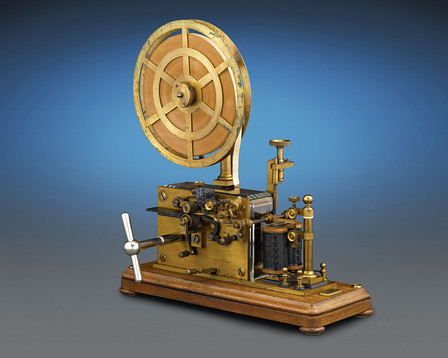
\includegraphics[margin=2em, width=0.4\textwidth]{figuras/Morse_Code_Receiver.png} &
        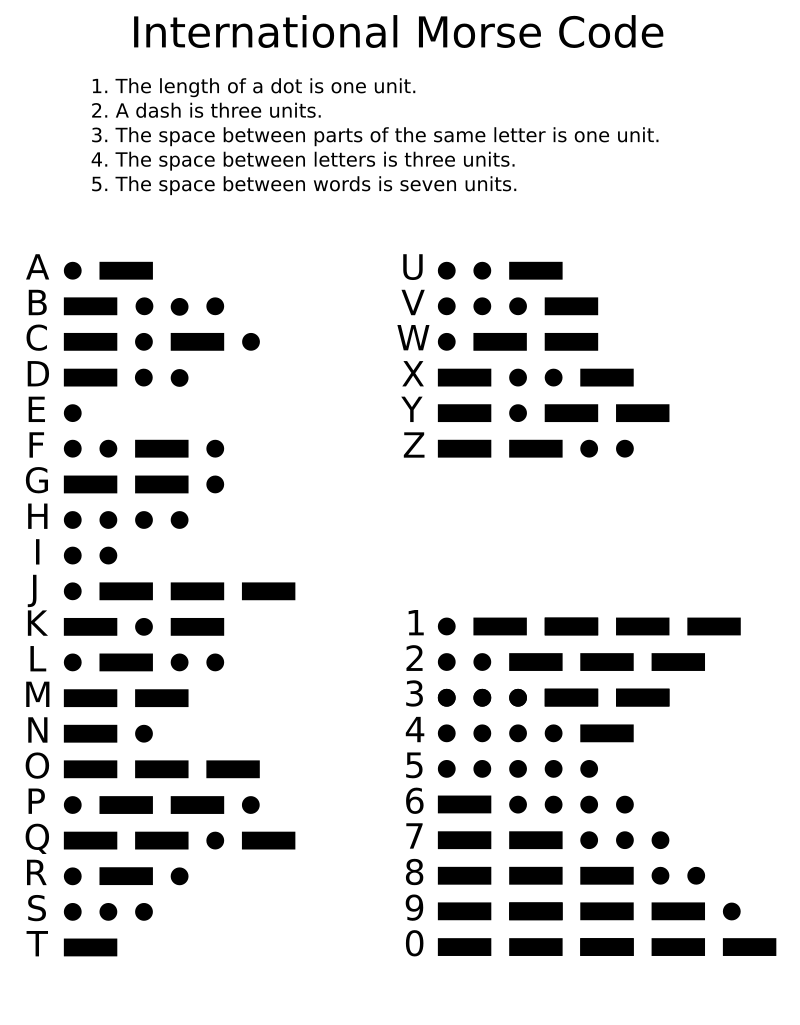
\includegraphics[margin=2em, width=0.3\textwidth]{figuras/International_Morse_Code.png}
        \end{tabular}
    \end{center}
    \caption{Telégrafo de Morse.}\label{fig:morse}
\end{figure}

Para entender las ventajas de la comunicación digital, es bueno remitirse primero a un esquema básico de comunicación analógico, como el mostrado en la Figura \ref{fig:analogico}. Allí, la fuente de información (ej. audio) es transformada en una señal eléctrica continua $x(t)$ por un transductor (ej. micrófono). El sistema de modulación intentará transmitir dicha señal por un medio físico, recibiendo $\hat{x}(t)$, señal que luego es enviada a otro transductor (ej. parlante) para enviarla al receptor. El objetivo de este proceso es que la señal $\hat{x}(t)$ reproduzca lo más fielmente posible la señal original $x(t)$, en todo momento del tiempo. Sin embargo, esto resulta imposible debido a que el canal siempre introduce atenuación, limitaciones de ancho de banda, potencia de transmisión y ruido que alteran la recepción (en algunos casos hasta volverla inservible).

En la transmisión digital, se transmiten símbolos $a_k$ construyendo una señal real $x(t)$ que depende de dichos símbolos. Si la señal recibida $\hat{x}(t)$ es suficientemente inteligible, podemos decodificar el símbolo $\hat{a}_k$ con \emph{muy  alta probabilidad} de que sea exactamente igual a $a_k$. En ese caso, la reconstrucción de la señal es perfecta (con alta probabilidad). Es decir, \emph{no hay pérdida de información por atravesar el canal}. Esto vuelve la transmisión mucho más robusta al ruido e interferencia. El objetivo principal de este curso es entender precisamente cómo realizar este proceso.

\begin{figure}
    \begin{center}
        
        \begin{blockdiagram}
        \node [block] (fuente) {Fuente};
        \node [block, right = of fuente] (transducer) {Transductor};
        \node [block, right = 6em of transducer] (tx) {Transmisor};
        \node [block, below = of tx] (ch) {Canal};
        \node [block, below = of ch] (rx) {Receptor};
        \node [block, left = 6em of rx] (transducer2) {Transductor};
        \node [block, left = of transducer2] (sink) {Receptor};
        \draw[thick, ->] (fuente)--(transducer);
        \draw[thick, ->] (transducer)--node[midway, above] {$x(t)$} (tx);
        \draw[thick, ->] (tx)--(ch);
        \draw[thick, ->] (ch)--(rx);
        \draw[thick, ->] (rx)--node[midway, above] {$\hat{x}(t)$} (transducer2);
        \draw[thick, ->] (transducer2)--(sink);
        \begin{scope}[on background layer]
            \node[draw, rectangle, dashed, fill=gray!25!white, fit=(tx) (ch) (rx), inner sep=10pt, label=below:Moduladción analógica] (modulador) {};
        \end{scope}

        \end{blockdiagram}
        \caption{Diagrama general de un sistema de transmisión analógico.}\label{fig:analogico}
    \end{center}
\end{figure}

Complementario a lo anterior existen dos fuertes razones para analizar la transmisión digital de datos:
\begin{enumerate}
    \item En primer lugar, en los últimos años, casi toda la información se almacena en forma digital (texto, fotos, video). En ese sentido, la información ya se encuentra en un alfabeto de símbolos (ej. binario) y no tiene sentido plantearse pasar por una etapa analógica, salvo para efectivamente transmitir sobre el medio físico.
    
    \item En otros casos, la señal analógica se convierte en una señal digital mediante un conversor analógico/digital (A/D) (Figura \ref{fig:a/d}) Aquí se cumplen dos etapas:
     \begin{enumerate}
        \item Se \emph{muestrea la señal} a una frecuencia de muestreo $f_s$ (muestras por segundo).
        \item Se \emph{cuantifica la señal} pasando el valor analógico a una cierta cantidad de símbolos (bits). Por ejemplo, las señales de audio se muestrean a $f_s=44100 \unit{Hz}$ y se digitalizan utilizando $16$ bits de resolución para cada canal estéreo. El resultado es una secuencia de muestras $a_k$ de $\approx 1.41 \unit{\mega bps}$.
     \end{enumerate}
\end{enumerate}

\begin{figure}
    \begin{center}        
        \begin{blockdiagram}
        \node [block, align=center] (fuente) {Fuente \\ analógica};
        \node [block, right = 5em of fuente, align=center, label=below:{Frec: $f_s$, $N$ bits}] (ad) {Conversor \\ A/D};
        \node [right = 5em of ad] (salida) {$Nf_s \unit{bps}$};
        \draw[thick, ->] (fuente)--node[midway,above] {$x(t)$} (ad);
        \draw[thick, ->] (ad)--node[midway, above] {$a_k$} (salida);
        \end{blockdiagram}
        \caption{Conversión analógica a digital.}\label{fig:a/d}
    \end{center}
\end{figure}

En el segundo caso, por el Teorema de Nyquist del muestreo, sabemos que si la señal $x(t)$ tiene ancho de banda $B$, entonces obteniendo muestras a frecuencia $f_s>2B$ es posible reconstruir la señal de manera \emph{exacta} a partir de las muestras $x(kT_s)$ con $T_s=1/f_s$. Sin embargo, como las muestras están cuantificadas, $a_k\approx x(kT_s)$ pero no es exacto, introduciendo el llamado \emph{ruido de cuantificación}. Este ruido es menor a mayor cantidad de bits utilizados para representar las muestras. Sin embargo, si la transmisión digital permite reconstruir las muestras $a_k$ exactamente, es probable que dicho ruido de cuantificación sea menor que el que introduce un esquema de modulación analógico, por lo cual la señal se recibe de mejor manera. A su vez, con los esquemas de modulación modernos, es posible aprovechar mejor el ancho de banda mandando más información (bits) sobre el mismo, por lo cual podemos realizar transmisiones de calidad.

\section{Diagrama general de un sistema de transmisión digital}

El diagrama general de un sistema de transmisión digital se muestra en la Figura \ref{fig:digital}. Allí partimos de una fuente ya digital que genera símbolos $\{a_k\}$, y se pasa por dos etapas de codificación que explicaremos. Con ello se genera una nueva señal digital $\{b_k\}$ que se enviará por el medio físico. Para ello, se requiere una etapa de \emph{modulación digital}, en la cual los símbolos $b_k$ se convierten en una señal analógica adecuada, se envían por el canal, y luego son reconstruidos por un \emph{detector} digital, que obtiene una secuencia $\hat{b}_k$. El objetivo de esta etapa es lograr que $\p{\hat{b}_k=b_k}$ sea máxima, de este modo permitiendo reconstruir la señal. Luego esta se decodifica por el proceso inverso a la codificación para obtener $\hat{a}_k$ y enviar esta señal al receptor. 

\begin{figure}
    \begin{center}
        
        \begin{blockdiagram}[node distance=3em]
        \node [block,align=center] (fuente) {Fuente \\ digital};
        \node [block, right = 5em of fuente, align=center] (codfuente) {Cod. de fuente};
        \node [block, right = of codfuente, align=center] (codcanal) {Cod. de canal};
        \node [block, right = 5em of codcanal] (tx) {Transmisor};
        \node [block, below = of tx] (ch) {Canal};
        \node [block, below = of ch] (rx) {Receptor};
        \node [block, left = 5em of rx] (decocanal) {Decod. canal};
        \node [block, left = of decocanal] (decofuente) {Decod. fuente};
        \node [block, left = 5em of decofuente, align=center] (sink) {Receptor \\ digital};

        \draw[thick, ->] (fuente)--node[midway,above] {$a_k$} (codfuente);
        \draw[thick, ->] (codfuente)--(codcanal);
        \draw[thick, ->] (codcanal)--node[midway,above] {$b_k$} (tx);
        \draw[thick, ->] (tx)--node[midway,right] {$x(t)$} (ch);
        \draw[thick, ->] (ch)--node[midway,right] {$\hat{x}(t)$} (rx);
        \draw[thick, ->] (rx)--node[midway,above] {$\hat{b}_k$} (decocanal);
        \draw[thick, ->] (decocanal)--(decofuente);
        \draw[thick, ->] (decofuente)--node[midway,above] {$\hat{a}_k$} (sink);
        
        \node [block, right = of ch] (sinc) {Sincronismo};
        \draw[thick, -] (tx) -| (sinc);
        \draw[thick, ->] (sinc) |- (rx);

        \begin{scope}[on background layer]
            \node[draw, rectangle, dashed, fill=gray!25!white, fit=(tx) (ch) (rx) (sinc), inner sep=10pt, label=below:Moduladción digital] (modulador) {};
            \node[draw, rectangle, dashed, fill=gray!25!white, fit=(codfuente) (codcanal), inner sep=10pt, label=below:Etapa de codificación] (cod) {};
            \node[draw, rectangle, dashed, fill=gray!25!white, fit=(decofuente) (decocanal), inner sep=10pt, label=below:Etapa de decodificación] (decod) {};

        \end{scope}
        \end{blockdiagram}

        \caption{Diagrama general de un sistema de transmisión digital.}\label{fig:digital}
    \end{center}
\end{figure}

El objetivo de este curso es analizar la etapa de \emph{modulación digital}, es decir dada una secuencia de símbolos $\{b_k\}$, cómo construir una señal analógica $x(t)$ que contenga la información de dichos símbolos y sea adecuada para su transmisión por el medio físico (radio, par de cobre, fibra óptica). Luego de su transmisión, la señal alterada deberá ser detectada y de allí reconstruiremos una secuencia de símbolos con baja probabilidad de error. El término modulación digital hace referencia a que la señal discreta \emph{modula} características de la señal analógica. Notemos además que este proceso requiere un bloque adicional: el \emph{sincronismo}, para que el receptor sepa a qué velocidad se transmite la información y cuál es el mejor momento del tiempo para muestrear la señal $\hat{x}(t)$ de manera de recuperar $\hat{b}_k$.

Si bien en este curso no trabajaremos sobre la etapa de \emph{codificación}, es importante entender el rol que cumplen las mismas previo a la transmisión. Introducimos ahora los principales conceptos.

\section{Conceptos básicos de codificación}

Como se observa en la Figura \ref{fig:digital}, existen dos etapas: la \emph{codificación de fuente} y la \emph{codificación de canal}, con sus respectivos decodificadores.

\subsection{Codificación de fuente}

El objetivo de la codificación de fuente es \emph{eliminar redundancia} de los datos, produciendo una secuencia de símbolos con menor cantidad de ``bits por símbolo'', de manera de requerir menor velocidad de transmisión de información. Existen dos tipos:
\begin{description}
    \item[Codificación sin pérdida:] Aquí la secuencia de símbolos generada contiene toda la información de la señal $\{a_k\}$, pero \emph{comprimida}. Esto es, utilizando propiedades estadísticas de la señal, se logra representar la misma información con menos bits. Un ejemplo de esto es el algoritmo \href{https://en.wikipedia.org/wiki/LZ77_and_LZ78}{Lempel-Ziv}, utilizado en la compresión ``.zip''.
    
    \item[Codificación con pérdida:] Aquí la secuencia de símbolos generada contiene \emph{menos información} que la original, eliminando por ejemplo partes que no son requeridas por el receptor. Ejemplos de esto son la compresión de imágenes JPEG, la compresión de video MPEG y la codificación de audio MP3. En estos casos, la señal reconstruida es una ``buena aproximación'' de la información original. Qué quiere decir ``buena aproximación'' depende de la aplicación, pero a modo de ejemplo el MP3 permite reducir la velocidad de audio mencionada anteriormente ($1.41 \unit{\mega bps}$) a $192 \unit{\kilo bps}$ o menos sin que el usuario detecte mayormente la diferencia. 
\end{description}

\begin{ejemplo}[Codificación sin pérdida]\label{ej:lossless}
Consideremos una fuente de datos que genera símbolos \emph{independientes} con la siguiente estadística:
\begin{equation*}
    a_k \in \{0,1,2,3\} \text{ con distribución } \begin{cases}
    \p{a_k=0} = 1/2 \\
    \p{a_k=1} = 1/4 \\
    \p{a_k=2} = 1/8 \\
    \p{a_k=3} = 1/8 \\
    \end{cases}
\end{equation*}
En este caso, una codificación sencilla sería tomar el código:
\begin{equation*}
    \begin{cases}
        a_k = 0 \mapsto \tilde{a}_k = 00 \\
        a_k = 1 \mapsto \tilde{a}_k = 01 \\
        a_k = 2 \mapsto \tilde{a}_k = 10 \\
        a_k = 3 \mapsto \tilde{a}_k = 11 \\
    \end{cases}
\end{equation*}
Observemos que el código anterior requiere en promedio 2 bits por símbolo (ya que todos los códigos son de 2 bits). ¿Podemos hacerlo mejor? Consideremos el siguiente código, debido a \href{https://en.wikipedia.org/wiki/Huffman_coding}{Huffman}:
\begin{equation*}
    \begin{cases}
        a_k = 0 \mapsto \tilde{a}_k = 0 \\
        a_k = 1 \mapsto \tilde{a}_k = 10 \\
        a_k = 2 \mapsto \tilde{a}_k = 110 \\
        a_k = 3 \mapsto \tilde{a}_k = 111 \\
    \end{cases}
\end{equation*}

Notemos que el código anterior es un \emph{código de prefijo} (cada símbolo empieza de manera diferente), lo que permite que sea invertible. Es decir si por ejemplo recibimos:
\begin{equation*}
    0101001110110111 \mapsto 0\;10\;10\;0\;111\;0\;110\;111 \mapsto 01103023
\end{equation*}
Calculemos el largo medio de la palabra enviada de la siguiente forma, donde $\ell(\cdot)$ representa el largo del código:
\begin{align*}
    \bar{L} &= \p{a_k=0} \ell(0) + \p{a_k=1} \ell(10) + \p{a_k=2} \ell(110) + \p{a_k=3} \ell(111)\\
    &= \left(\frac{1}{2}\right)(1) + \left(\frac{1}{4}\right)(2) + \left(\frac{1}{8}\right)(3) + \left(\frac{1}{8}\right)(3) = 1.75 < 2
\end{align*}

Esto quiere decir que en el largo plazo, una secuencia de $N$ símbolos podrá ser representada por $\approx 1.75 N$ bits (en lugar de $2N$), permitiendo un ahorro.
\end{ejemplo}

La clave del ejemplo anterior está en elegir palabras más largas para símbolos menos frecuentes. Notemos que esto mismo ya había sido advertido por Morse en su código, como se ve en la Figura \ref{fig:morse}. Surgen entonces las siguientes preguntas: ¿cuál es el mínimo largo medio posible de codificación? ¿Es alcanzable?

En 1948, \href{https://en.wikipedia.org/wiki/Claude_Shannon}{Claude Shannon} establece la teoría matemática de transmisión de información, introduciendo el concepto de \emph{entropía} de una fuente. Dicha entropía representa la cantidad de información contenida en una fuente (considerando sus propiedades estadísticas). Para una fuente $X$ que genera símbolos independientes $\{a_k\}$, la misma se define como:
\begin{equation*}
    H(X) = -\sum_k p_k \log_2(p_k)
\end{equation*}
siendo $p_k$ la probabilidad de cada símbolo y $\log_2$ el logaritmo en base $2$, lo que hace que la entropía quede en bits/símbolo.

Calculemos la entropía de la fuente anterior:
\begin{equation*}
    H(X) = \left(\frac{1}{2}\right)(1) + \left(\frac{1}{4}\right)(2) + \left(\frac{1}{8}\right)(3) + \left(\frac{1}{8}\right)(3) = 1.75.
\end{equation*}
Es decir, recuperamos exactamente el largo medio del código de Huffman anterior.

\begin{ejemplo}[Fuente binaria]\label{ej:entropia binaria}
    Supongamos que los símbolos son binarios $a_k\in\{0,1\}$ con $\p{a_k=1} = p = 1-\p{a_k=0}$ e independientes. En ese caso la entropía queda (como función de $p$):
    \begin{equation}\label{eq:entropia binaria}
        H(p) = -p\log_2 (p) - (1-p) \log_2(1-p),
    \end{equation}
    cuya gráfica puede verse en la Figura \ref{fig:entropia binaria}.
\end{ejemplo}


\begin{figure}
    \begin{center}
        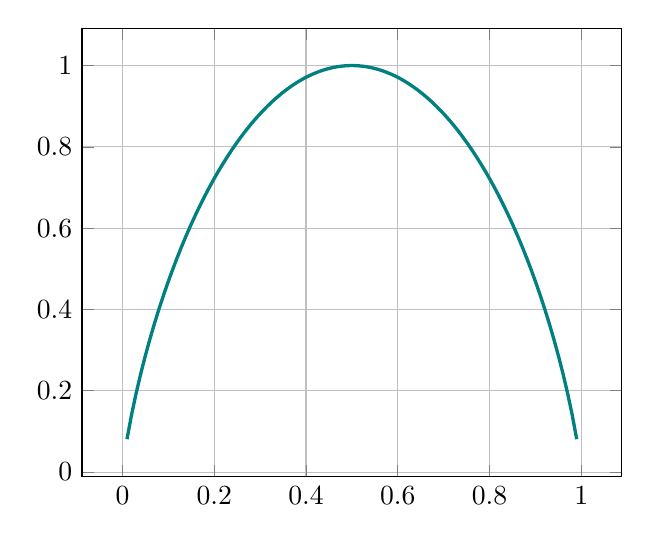
\begin{tikzpicture}
            \begin{axis}[grid]
            \addplot[domain=0.01:.99,samples=100, color=teal, very thick] {-x*ln(x)/ln(2) - (1-x)*ln(1-x)/ln(2)};
            \end{axis}
        \end{tikzpicture}
    \end{center}
    \caption{Entropía de una fuente binaria. Notar que el máximo se alcanza para $p=1/2$, es decir, distribución uniforme.}\label{fig:entropia binaria}
\end{figure}

El Teorema de Shannon muestra que para una fuente dada, su entropía es la mínima cantidad de bits por símbolo alcanzable:
\begin{teorema}[Shannon, 1948]
Sea una fuente de símbolos $\{a_k\}$ y su entropía $H_a$. Entonces es posible agrupar los símbolos de a bloques de tamaño $N$ y codificarlos en palabras de $L_N$ bits de manera que el largo medio de palabra cumpla:
\begin{equation*}
    N H_a \leqslant \bar{L}_N \leqslant NH_a + 1 
\end{equation*}
Como cada bloque codifica $N$ símbolos, la cantidad de bits por símbolo será entonces:
\begin{equation*}
    H_a \leqslant \frac{\bar{L}}{N} \leqslant H_a + 1/N
\end{equation*}
Además, no existe ningún código que logre mejorar esta cota.
\end{teorema}

La entropía de una fuente nos entonces da la mínima cantidad de bits por símbolo que podemos utilizar, es decir, el límite de la compresión alcanzable. Si volvemos al Ejemplo \ref{ej:lossless}, vemos que precisamente el código de Huffman alcanza la mínima entropía posible, incluso con $N=1$. Para otras distribuciones puede ser necesario utilizar un largo mayor de bloque para aproximar la entropía.

En el Ejemplo \ref{ej:entropia binaria}, vemos que la entropía es máxima e igual a $1$ cuando los símbolos son \emph{equiprobables} ($p=1/2$). En ese caso, debemos utilizar 1 bit por símbolo y la señal es incompresible. Precisamente, el código de Huffman descrito logra que la fuente original genere cantidades equiprobables de $0$ y $1$, por lo cual no puede comprimirse más.

Si en cambio $p\to 0$, la fuente tiene secuencias largas de $0$, y en ese caso puede ser más eficiente codificar el largo de la cadena de $0$s que indicar cada bit por separado. En el caso extremo, solo alcanza 1 bit para toda la cadena (``son todos ceros''). Análogamente, si $p\to 1$.

\subsection{Codificación de canal}

El objetivo de la codificación de fuente es reducir la cantidad de datos a transmitir a su mínima expresión, eliminando redundancia sin pérdida de información (o en el caso con pérdida, sin distorsión relevante). La \emph{codificación de canal} va en sentido opuesto: agrega redundancia para anticiparse a posibles errores del canal de transmisión y poder detectarlos y corregirlos. A continuación damos algunos ejemplos.

\begin{ejemplo}[Bit de paridad]\label{ej:paridad}
    Supongamos una fuente binaria $\{a_k\}$ y formemos bloques de largo $N$. Al final de cada bloque se agrega un bit $a_N = a_0 \oplus \ldots \oplus a_{N-1}$ donde $\oplus$ es la operación XOR. Luego se transmite la palabra $b = (a_0,\ldots,a_N)$. El resultado final es que $a_N=1$ si hay una cantidad impar de $1$s en el bloque, o dicho de otro modo, cada bloque $b$ tiene una cantidad par de bits. Esto permite \emph{detectar} (pero no corregir) errores de $1$ bit, con un overhead de $1/N$ bits por símbolo.

    Obviamente, si el largo de bloque $N$ es grande, el overhead es mínimo, pero la probabilidad de que haya errores de más de un bit es mayor, por lo cual la elección de $N$ es un compromiso entre ambos efectos.
\end{ejemplo}

\begin{ejemplo}[Código de repetición]\label{ej:codrep}
    Supongamos una fuente binaria $\{a_k\}$ y realicemos el siguiente procedimiento: para cada símbolo $a_k$ formamos un bloque $b=(a_k, a_k, a_k)$. Esto es un código de repetición de largo $3$. Observemos que si hay un error de $1$ bit, podemos decidir por mayoría si el bloque corresponde a un $0$ o a un $1$. Por ejemplo $(110)\mapsto 1$ y $(010)\mapsto 0$. Esto permite \emph{detectar y corregir} errores de $1$ bit. Sin embargo, requiere 3 bits por símbolo, lo cual es ineficiente.
\end{ejemplo}

\begin{ejemplo}[Matriz de paridad]\label{ej:parity matrix}
    Consideremos ahora el siguiente procedimiento para una fuente binaria $\{a_k\}$. Elegimos un número $M$ y formamos bloques de tamaño $N=M^2$ dispuestos en forma de matriz de $M\times M$. Luego se agrega a dicha matriz un bit de paridad para cada fila y cada columna, así como un bit de paridad total. Por ejemplo, si $M=4$, $N=16$:
    \begin{equation*}
        (1001000111111011) \; \mapsto\; \begin{pmatrix}
            1 & 0 & 0 & 1 \\
            0 & 0 & 0 & 1 \\
            1 & 1 & 1 & 1 \\
            1 & 0 & 1 & 1 \\
        \end{pmatrix} \; \mapsto \; \begin{pmatrix}
            1 & 0 & 0 & 1 & \vdots & 0 \\
            0 & 0 & 0 & 1 & \vdots & 1 \\
            1 & 1 & 1 & 1 & \vdots & 0 \\
            1 & 0 & 1 & 1 & \vdots & 1 \\
            \cdots & \cdots & \cdots & \cdots & \cdots & \cdots \\
            1 & 1 & 0 & 0 & \vdots & 0 \\
        \end{pmatrix}
    \end{equation*}
    Luego se envían los $N$ bits y los $M+1$ bits de paridad agregados.

    Si hay un error de un bit, el mismo se \emph{detecta} y se \emph{corrige} porque los errores de paridad indican la fila y columna del error, por ejemplo:
    \begin{equation*}
         \begin{pmatrix}
            1 & 0 & 0 & 1 & \vdots & 0 \\
            0 & 0 & 0 & 1 & \vdots & 1 \\
            1 & 1 & 1 & 1 & \vdots & 0 \\
            1 & 0 & 1 & 1 & \vdots & 1 \\
            \cdots & \cdots & \cdots & \cdots & \cdots & \cdots \\
            1 & 1 & 0 & 0 & \vdots & 0 \\
        \end{pmatrix} \; \rightsquigarrow  \;
         \begin{pmatrix}
            1 & 0 & 0 & 1 & \vdots & 0 \\
            0 & 0 & {\color{red} 1} & 1 & \vdots & 1{\color{red} *} \\
            1 & 1 & 1 & 1 & \vdots & 0 \\
            1 & 0 & 1 & 1 & \vdots & 1 \\
            \cdots & \cdots & \cdots & \cdots & \cdots & \cdots \\
            1 & 1 & 0{\color{red} *} & 0 & \vdots & 0 \\
        \end{pmatrix}
    \end{equation*}
    El código detecta entonces donde ocurrió el error porque la paridad de la fila y la columna no es correcto. Notar que el error también puede ocurrir en la fila o en la columna de paridad. Esto también se detecta y se corrige gracias al bit extra de paridad total.

    El resultado es que se envían $N$ bits con una redundancia de $2M+1 = 2\sqrt{N} + 1$ por lo que en un bloque de $N=1024$ bits solo se requieren $65$ bits extra. El overhead crece más lento que el tamaño de bloque. De todos modos sigue siendo ineficiente y solo permite corregir errores de $1$ bit, por lo que si el tamaño de bloque es grande, tenemos el mismo problema que en Ejemplo \ref{ej:paridad}.
\end{ejemplo}

El punto común de todos los ejemplos anteriores es el siguiente: dado un alfabeto de símbolos (por ejemplo binario), construimos bloques de largo $N$. Esto permite generar $2^N$ símbolos posibles. Luego agregamos bits de control, generando palabras de largo $N+r$, y aplicando un código que lleva secuencias de largo $N$ a un \emph{espacio mayor} de largo $N+r$, donde los códigos ``válidos'' se encuentran \emph{más separados entre sí} (solo hay $2^N$ palabras válidas de las $2^{N+r}$ posibles). Cuando ocurre algún error, encontramos una palabra no válida y detectamos el error. Si el código es adecuado, podemos además mapear esa palabra no válida a un símbolo válido ``cercano'' corrigiendo entonces el error.

A mayor $r$, más redundancia se agrega, más espacio se genera, y podemos detectar y corregir errores más grandes. Pero por otra parte, el overhead es mayor. Se le denomina \emph{tasa de codificación (code rate)} al cociente $N/(N+r)$.

Un ejemplo de código de este tipo son los \href{https://en.wikipedia.org/wiki/Hamming_code}{Códigos de Hamming}, en los cuales se elige un tamaño de bloque $N+r=2^{r}-1$ con $r\geqslant 1$ y se envía un mensaje de largo $N=2^{r} - r - 1$ con $r$ bits de redundancia, utilizando una transformación lineal invertible. En ese caso, la tasa de codificación queda:
\begin{equation*}
    R = 1-\frac{r}{2^r-1},
\end{equation*}
es decir, la redundancia es del orden de $\log_2(N)\ll \sqrt{N}$. Sin embargo, si bien es más eficiente que la matriz de paridad, este código solo permite detectar errores de 1 o 2 bits, y corregir errores de un único bit. El tipo más común de código de bloques es el de \href{https://en.wikipedia.org/wiki/Reed\%E2\%80\%93Solomon_error_correction}{Reed--Solomon, 1960}, una familia de códigos que permite detectar errores de hasta $r$ bits y corregir hasta $\lfloor r/2 \rfloor$ bits, siendo $r$ un parámetro, la cantidad de redundancia deseada. Es además capaz de recuperar errores de ``borrado'', donde no es posible decidir si el bit recibido es $0$ o $1$.

Más recientemente, la aparición de los \href{https://en.wikipedia.org/wiki/Convolutional_code}{códigos convolucionales}, \href{https://en.wikipedia.org/wiki/Turbo_code}{Turbo--codes} y códigos \href{https://en.wikipedia.org/wiki/Low-density_parity-check_code}{Low--Parity--Data--Check}, se logran tasas de codificación cercanas a $1$ con muy baja probabilidad de error. 



\chapter{Procesos aleatorios}\label{chapter:procesos estocasticos}
En el estudio de la transmisión de señales (analógicas o digitales), es necesario diseñar el sistema para transmitir información que, a priori, no es conocida en detalle. Por ejemplo, la señal de voz de la radio AM/FM no se conoce hasta el momento de la transmisión. Lo mismo ocurre en la transmisión digital: típicamente podemos conocer \emph{estadísticamente} como se comportan los datos, pero no exactamente qué es lo que se va a transmitir. Debemos entonces poder diseñar y analizar los sistemas de transmisión para que respondan de manera adecuada a este conjunto posible de señales, de las cuales no conocemos exactamente más que sus propiedades estadísticas.

Es por ello esencial introducir el concepto de \emph{proceso estocástico} o aleatorio, que permite modelar este comportamiento. Comenzaremos en tiempo discreto para luego pasar a tiempo continuo, ya que ambos serán necesarios en el estudio de la modulación digital. Remitimos al apéndice \ref{app:probabilidad} para un resumen de los conceptos previos requeridos de probabilidad y variables aleatorias.

\section{Proceso estocástico de tiempo discreto}

Comencemos por definir el objeto de trabajo:
\begin{definicion}\label{def:proceso_td}
    Un \emph{proceso estocástico de tiempo discreto} es una sucesión de variables aleatorias $\{a_k:k\in\mathbb{Z}\}$ definidas en un espacio de probabilidad y que toman valores en un conjunto de símbolos $\{s_1,\ldots,s_M\}$ (espacio discreto) o valores en $\mathbb{R}$ (espacio continuo).
\end{definicion}

Observemos que la definición anterior no implica que los símbolos o muestras $a_k$ son independientes entre sí, es decir, pueden tener \emph{correlación} entre ellas. La distribución de un proceso estocástico depende precisamente de cuál es la probabilidad de observar cualquier secuencia de símbolos. En general esto es difícil de calcular por lo que definiremos algunas magnitudes de interés.

\begin{definicion}\label{def:media_var_td}
    Se definen la \emph{media} y \emph{varianza} del proceso como:
    \begin{equation*}
        \mu_k := \E{a_k}, \quad \sigma^2_k := \E{(a_k-\mu_k)^2} = \E{a_k^2} - \mu_k^2.
    \end{equation*}
    Por último definimos la \emph{potencia} del proceso como:
    \begin{equation*}
        P_k := \E{a_k^2} = \mu_k^2 + \sigma_k^2.
    \end{equation*}
\end{definicion}
Notar que en principio estas dependen de $k$, que es el índice de tiempo. Esto es, si la estadística del proceso cambia a lo largo del tiempo, también lo harán estas magnitudes.

Para capturar la dependencia del proceso introducimos la siguiente:
\begin{definicion}\label{def:autocorrelacion_noest_td}
    Se define la \emph{autocorrelación} de un proceso $\{a_k\}$ como:
    \begin{equation*}
        R(k_1,k_2) = \E{a_{k_1}a_{k_2}}
    \end{equation*}
\end{definicion}
Esta magnitud evalúa cuan ``alineados'' o ``similares'' son las muestras del proceso en los tiempos $k_1$ y $k_2$. En particular observemos que $R(k,k)=P_k$.

Sin embargo, todas estas magnitudes dependen del tiempo específico en que miremos. Es aquí que conviene introducir la noción de \emph{proceso estacionario}, que son aquellos procesos estocásticos cuyas propiedades estadísticas son invariantes en el tiempo, es decir la distribución de las observaciones $a_k$ o de las parejas $(a_{k_1},a_{k_2})$ no depende de $k$. En particular:
\begin{itemize}
    \item $\E{a_k} = \mu$, $\textrm{Var}(a_k)=\sigma^2$ y $P=\E{a_k^2}$ deben ser constantes.
    \item La autocorrelación satisface:
       \begin{equation*}
        R(k_1,k_2) = \E{a_{k_1}a_{k_2}} = \E{a_{0}a_{k_2-k_1}} = \E{a_{0}a_{l}} = R(0,l).
       \end{equation*}
       Es decir la autocorrelación solo depende de $l=k_2-k_1$, la distancia en el tiempo entre las observaciones o \emph{lag}.
\end{itemize}

A los efectos de trabajar con señales y modulación conviene entonces introducir la siguiente clase de procesos.
\begin{definicion}[Proceso WSS de tiempo discreto]
    Un proceso estocástico $\{a_k\}$ se dice \emph{estacionario en sentido amplio (WSS, wide-sense stationary)} si verifica:
    \begin{enumerate}
        \item $\E{a_k} = \mu$ constante.
        \item $R(a_{k_1},a_{k_2}) = R_a[k_2-k_1]$, siendo $R_a[l]$ una función únicamente del lag $l$, la distancia entre muestras.
    \end{enumerate}
\end{definicion}

\begin{ejemplo}[Variables aleatorias independientes]\label{ej:iid}
    Si las muestras $\{a_k\}$ son variables aleatorias independientes, de media $\mu$ y varianza $\sigma^2$ constantes, entonces se verifica la primera condición, y la autocorrelación además verifica:
    \begin{equation*}
        \E{a_k a_{k+l}} = \begin{cases}
        \E{a_k^2} = \mu^2 + \sigma^2 & \text{si }l=0, \\
        \E{a_k}\E{a_{k+\tau}} = \mu^2 & \text{si }l\neq 0.
        \end{cases}
    \end{equation*}
    Por lo tanto el proceso es WSS con $R_a[l] = \mu^2 + \sigma^2 \delta[l]$, siendo $\delta$ la delta de Dirac en tiempo discreto ($\delta[0]=1,\delta[l]=0, l\neq0$).

    \begin{center}
        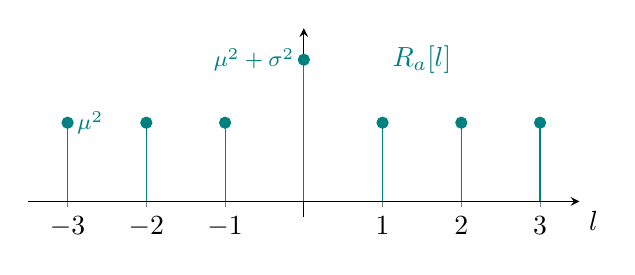
\begin{tikzpicture}
            \begin{axis}[ x=1cm, y=1cm, axis lines=middle,  
                    xlabel=$l$,
                    x label style={anchor=north west},
                    xmin=-3.5,xmax=3.5,ymin=-.2,ymax=2.2,
                    ytick=\empty,
                    clip=false,
                    ]
                \addplot+[teal,ycomb, mark options={teal}] plot coordinates {(-3,1) (-2,1) (-1,1) (0,1.8) (1,1) (2,1) (3,1)};
                \node[teal] at (axis cs:1.5,1.8) {$R_a[l]$};
                \node[teal,left] at (axis cs:0,1.8) {\footnotesize $\mu^2+\sigma^2$};
                \node[teal, right] at (axis cs:-3,1) {\footnotesize $\mu^2$};
            \end{axis}
        \end{tikzpicture}
    \end{center}
\end{ejemplo}

\begin{ejemplo}[Símbolos dependientes]\label{ej:markov source}
Consideremos una fuente que genera una secuencia de símbolos $\{a_k\}\in\{-1,1\}$ con la propiedad de que $\p{a_{k+1}=-1 \mid a_k=1} = \p{a_{k+1}=1 \mid a_k=-1} = \alpha$. Aquí $\alpha$ representa la probabilidad de ``cambiar de estado''. Si $\alpha\to 0$ la señal tiene rachas largas de $1$ y $-1$. Si $\alpha\to 1$ alterna periódicamente.

Es evidente que, en estado estacionario, por ser el sistema simétrico, $\p{a_k=1} = \p{a_k=-1} = 1/2$ por lo que en particular $\mu = \E{a_k} = 0$. La autocorrelación $R_a[l]$ puede calcularse por métodos que no veremos aquí y vale:
\begin{equation*}
    R_a[\tau] = (1-2\alpha)^{|l|}.
\end{equation*}

    \begin{center}
        \begin{tikzpicture}
            \begin{axis}[ x=1cm, y=1.2cm, axis lines=middle,  
                    xlabel=$l$,
                    x label style={anchor=north west},
                    xmin=-5.5,xmax=5.5,ymin=-.2,ymax=2,
                    ytick=\empty,
                    clip=false,
                    ]
                \addplot+[teal,ycomb, mark options={teal},samples = 11, domain=-5:5] {.5^abs(x)};
                \node[teal] at (axis cs:2.5,1.5) {$R_a[l], \; \alpha=1/4$};
            \end{axis}
        \end{tikzpicture}
    \end{center}

\end{ejemplo}

Listamos a continuación algunas propiedades de la autocorrelación:
\begin{enumerate}
    \item $R_a[l] = \E{a_k a_{k+l}} = \E{a_{k-l} a_k} = R_a[-l]$.
    \item $R_a[0] = \E{a_k^2} = P$.
    \item $|R_a[l]| = |\E{a_k a_{k+l}}| \leqslant \sqrt{\E{a_k^2}\E{a_{k+l}^2}} =\sqrt{P^2} = P = R_a[0]$. 
    
    Es decir, en módulo la autocorrelación es máxima en $0$. La desigualdad anterior surge de la desigualdad de Cauchy-Schwarz para variables aleatorias.
\end{enumerate}

La autocorrelación es la expresión temporal de cómo se repite (en promedio) la señal. Es por ello que a los efectos de analizar el filtrado y modulación de señales aleatorias interesa definir una expresión en el dominio de la frecuencia.

\begin{definicion}[Densidad espectral de potencia (tiempo discreto)]
    Se define la \emph{densidad espectral de potencia} de un proceso WSS de tiempo discreto con autocorrelación $R_a(\tau)$ como:
    \begin{equation}\label{def:dep_discreta}
        S_a(\phi) = \sum_{l=-\infty}^\infty R_a[l] e^{-j2\pi l \phi},
    \end{equation}
    es decir, la TFTD de la autocorrelación.
\end{definicion}

Esta función es periódica de período $1$ como función de $\phi$. La interpretación de $\phi$ es de \emph{frecuencia normalizada}, $f/f_s$ siendo $f_s$ la frecuencia de muestras de la señal. En general analizaremos el comportamiento de $S_a(\phi)$ para $\phi\in[-1/2,1/2]$ (correspondiente al intervalo $[-f_s/2,f_s/2]$ de frecuencias observables),

Al ser $S_a$ la TFTD de $R_a$, notemos que podemos recuperar la autocorrelación de la densidad espectral como:
\begin{equation*}
    R_a[l] = \int_{-\frac12}^{\frac12} S_a(\phi) e^{j2\pi l \phi} d\phi.
\end{equation*}

Algunas propiedades de la densidad espectral de potencia son:
\begin{enumerate}
    \item $S_a(\phi)$ es real y positiva.
    \item Para señales reales, $S_a(\phi)=S_a(-\phi)$ (función par).
    \item \begin{equation*}
    P = R_a[0] = \int_{-\frac12}^{\frac12} S_a(\phi) d\phi
    \end{equation*}
\end{enumerate}
Es decir, el área bajo la gráfica de $S_a$ (en un período) es igual a la potencia de la señal. En ese sentido, $S_a$ nos indica \emph{cómo se distribuye la potencia} a lo largo de las frecuencias observables.

\begin{ejemplo}
    Para el proceso independiente del Ejemplo \ref{ej:iid}, la densidad espectral de potencia queda:
    \begin{equation*}
        S_a(\phi) = \sum_{l=-\infty}^\infty \left[\mu^2 + \sigma^2 \delta(k)\right]e^{-j2\pi\phi\tau} = \sigma^2 + \mu^2 \sum_{l=-\infty}^\infty e^{-j2\pi\phi\tau} = \sigma^2 + \mu^2 \sum_{l=-\infty}^\infty \delta(\phi-l),
    \end{equation*}
donde en el último paso usamos la suma de Poisson.
    \begin{center}
    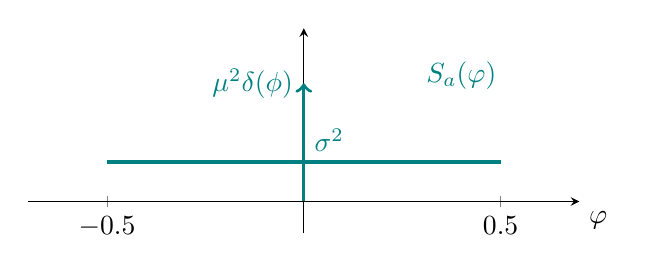
\begin{tikzpicture}
        \begin{axis}[ x=5cm, y=2cm, axis lines=middle,  
                xlabel=$\varphi$,
                x label style={anchor=north west},
                xmin=-.7,xmax=.7,ymin=-.2,ymax=1.1,
                ytick=\empty,
                xtick = {-.5,.5},
                clip=false,
                ]
            \addplot[teal, samples = 100, domain=-.5:.5, very thick] {1/4} node[midway,above right] {$\sigma^2$};
            \node[teal] at (axis cs:.4,.8) {$S_a(\varphi)$};
            \draw[teal,very thick, ->] (axis cs:0,0) -- (axis cs:0,.75) node[left] {$\mu^2 \delta(\phi)$};
        \end{axis}
    \end{tikzpicture}
\end{center}

\end{ejemplo}

\begin{ejemplo}
    Para la señal aleatoria con símbolos dependientes del Ejemplo \ref{ej:markov source}, la densidad espectral de potencia queda:
    \begin{align*}
        S_a(\phi) &= \sum_{\tau = -\infty}^\infty (1-2\alpha)^{|\tau|} e^{-j2\pi\phi \tau} = 1 + \sum_{l=1}^\infty \left[(1-2\alpha)e^{-j2\pi\phi }\right]^l + \sum_{l=1}^\infty \left[(1-2\alpha)e^{j2\pi\phi}\right]^l \\
        &= 1 + \frac{(1-2\alpha)e^{-j2\pi\phi}}{1-(1-2\alpha)e^{-j2\pi\phi}} + \frac{(1-2\alpha)e^{j2\pi\phi}}{1-(1-2\alpha)e^{j2\pi\phi}}\\
        &= \frac{2\alpha(1-\alpha)}{1-2\alpha(1-\alpha) - (1-2\alpha)\cos(2\pi\phi)}.
    \end{align*}

    Por ejemplo, para $\alpha=1/4$ queda:
    \begin{center}
        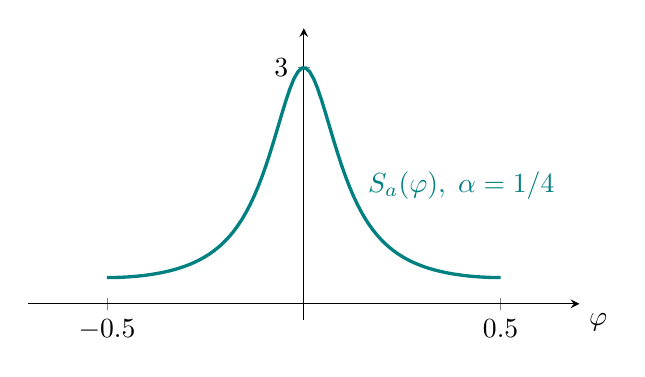
\begin{tikzpicture}
            \begin{axis}[ x=5cm, y=1cm, axis lines=middle,  
                    xlabel=$\varphi$,
                    x label style={anchor=north west},
                    xmin=-.7,xmax=.7,ymin=-.2,ymax=3.5,
                    ytick={3},
                    xtick = {-.5,.5},
                    clip=false,
                    ]
                \addplot[teal, samples = 100, domain=-.5:.5, very thick] {(3/8)/(1-(3/8)-(1/2)*cos(deg(2*pi*x)))};
                \node[teal] at (axis cs:.4,1.5) {$S_a(\varphi), \; \alpha=1/4$};
            \end{axis}
        \end{tikzpicture}
    \end{center}
\end{ejemplo}

Por último, introducimos una última noción:
\begin{definicion}
    Un proceso es \emph{ergódico} si una realización cualquiera es representativa de la estadística del proceso.
\end{definicion}

La anterior es una definición informal, pero la idea general es que si promediamos los valores de una traza del proceso, entonces recuperamos los valores medios. En particular:
\begin{align*}
    \left\langle a \right\rangle  &= \lim_{N\to\infty} \frac{1}{2N+1}\sum_{k=-N}^N a_k = E[a_k] = \mu, \\
    \left\langle a^2 \right\rangle &= \lim_{N\to\infty} \frac{1}{2N+1}\sum_{k=-N}^N a_k^2 = E[a_k^2] = P, \\
    \left\langle a_k a_{k+l}\right\rangle &= \lim_{N\to\infty} \frac{1}{2N+1}\sum_{k=-N}^N a_k a_{k+l} = E[a_k a_{k+l}] = R_a[l].
\end{align*}
Es decir, los valores medios de una señal dada suficientemente larga aproximan la esperanza, similar a lo que ocurre en la ley de grandes números. En particular se requiere estacionariedad (porque el límite no depende de $k$). En este curso asumiremos siempre que los procesos con que trabajamos son WSS y ergódicos.

\section{Proceso estocástico de tiempo continuo}

Generalizamos ahora las definiciones ya vistas al caso de tiempo continuo, lo que nos servirá por ejemplo para modelar señales analógicas que son moduladas por una señal digital, o también el ruido que afecta a un sistema.

\begin{definicion}\label{def:proceso_tc}
    Un \emph{proceso estocástico de tiempo continuo} es una función aleatoria $x(t,\omega)$ a valores reales, con $\omega$ sorteada en un espacio de probabilidad.
\end{definicion}

La principal diferencia es que ahora el sorteo en el espacio determina toda una función $x(t)$ para cada posible realización del experimento (valor de $\omega$). En la FIgura \ref{fig:realizaciones} se muestra un ejemplo de esto. En general, denotaremos por $x(t)$ a la señal o proceso aleatorio, sin indicar la dependencia con el espacio de probabilidad subyacente.

\begin{figure}
    \begin{center}
        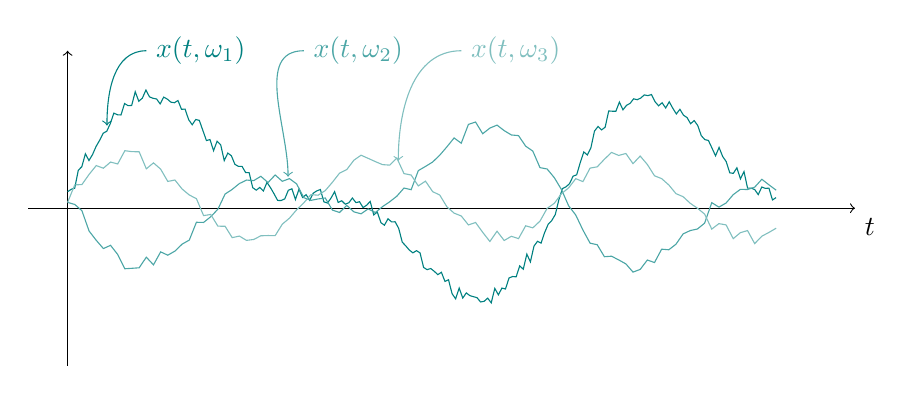
\begin{tikzpicture}
            \draw [->] (-0.5,0) -- (10,0) node[below right] {$t$};
            \draw [->] (0,-2) -- (0,2);
            \draw [samples=200,domain=0:9, teal] plot (\x,{0.15+sin(\x r)*(1+cos(\x r +1))+0.1*rand});
            \draw [->, teal] (1,2) node [anchor=west] {$x(t,\omega_1)$} to [out=180,in = 90] (0.5,1.05);
            \draw [samples=100,domain=0:9,color=teal!70!white] plot (\x, {0.15-sin(\x r)*(0.5+cos(\x r +1))+0.1*rand});
            \draw [->,color=teal!70!white] (3,2) node [anchor=west] {$x(t,\omega_2)$} to [out=180,in=90] (2.8,0.4);
            \draw [samples=100,domain=0:9,color=teal!50!white] plot (\x, {0.15+sin(\x r)*(cos(\x r +1))+0.1*rand});
            \draw [->,color=teal!50!white] (5,2) node [anchor=west] {$x(t,\omega_3)$} to [out=180,in=90] (4.2,0.6);
        \end{tikzpicture}
        \caption{Diferentes realizaciones de un proceso estocástico de tiempo continuo}\label{fig:realizaciones}
    \end{center}
\end{figure}

Dado un proceso estocástico $x(t)$, podemos definir:
\begin{definicion}\label{def:media_var_tc}
    Se definen la función \emph{media} y \emph{varianza} del proceso como:
    \begin{equation*}
        \mu(t) := \E{x(t)}, \quad \sigma^2(t) := \E{(x(t)-\mu(t))^2} = \E{x(t)^2} - \mu(t)^2.
    \end{equation*}
    Por último definimos la \emph{potencia} del proceso como:
    \begin{equation*}
        P(t) := \E{x(t)^2} = \mu(t)^2 + \sigma(t)^2.
    \end{equation*}
\end{definicion}

Tenemos a su vez el análogo a la autocorrelación de tiempo discreto.
\begin{definicion}\label{def:autocorrelacion_noest_tc}
    Se define la \emph{autocorrelación} de un proceso estocástico de tiempo continuo $x(t)$ como la función de dos variables:
    \begin{equation*}
        R(s,t) = \E{x(s)x(t)}.
    \end{equation*}
\end{definicion}
Observemos  que $R(t,t)=P(t)$.

Nuevamente, todas las magnitudes anteriores dependen en principio de los momentos del tiempo en que miramos el proceso. Buscamos entonces trabajar con procesos \emph{estacionarios} cuya estadística no cambie con el tiempo.
\begin{definicion}[Proceso WSS de tiempo continuo]
    Un proceso estocástico $x(t)$ se dice \emph{estacionario en sentido amplio (WSS, wide-sense stationary)} si verifica:
    \begin{enumerate}
        \item $\E{x(t)} = \mu$ constante.
        \item $R(s,t) = \E{x(s)x(t)} = \E{x(0)x(t-s)} =  R_x(\tau)$, siendo $R_x(\tau)$ una función únicamente de $\tau = t-s$, el tiempo entre muestras.
    \end{enumerate}
\end{definicion}

Tenemos además los análogos de tiempo continuo de la función de autocorrelación.\begin{enumerate}
    \item $R_x(\tau) = \E{x(t) x(t-\tau)} = \E{x(t+\tau)x(t)} = R_x(-\tau)$, es decir $R_x$ es una función par.
    \item $R_x(0) = \E{x(t)^2} = P$.
    \item $|R_x(\tau)| = |\E{x(t)x(t-\tau)}| \leqslant \sqrt{\E{x(t)^2}\E{x(t-\tau)}^2} =\sqrt{P^2} = P = R_a(0)$. 
Nuevamente, el módulo de la autocorrelación es máximo en $0$. La desigualdad anterior surge de la desigualdad de Cauchy-Schwarz para variables aleatorias.
\end{enumerate}

Por último, un proceso es además ergódico si cada trayectoria $x(t)$ es representativa de la estadística del proceso, como antes. En particular:
\begin{align*}
    \left\langle x \right\rangle  &= \lim_{T\to\infty} \frac{1}{2T}\int_{-T}^T x(t)dt = \E{x(t)} = \mu, \\
    \left\langle (x-\mu)^2 \right\rangle  &= \lim_{T\to\infty} \frac{1}{2T}\int_{-T}^T (x(t)-\mu)^2 dt = \E{(x(t)-\mu)^2} = \sigma^2, \\
    \left\langle x^2 \right\rangle &= \lim_{T\to\infty} \frac{1}{2T}\int_{-T}^T x(t)^2 dt = \E{x(t)^2} = P, \\
    \left\langle x(t) x(t-\tau) \right\rangle &= \lim_{T\to\infty} \frac{1}{2T}\int_{-T}^T x(t)x(t-\tau)dt = E[x(t)x(t-\tau)] = R_x(\tau).
\end{align*}
Es decir, los valores medios de una señal dada suficientemente larga aproximan la esperanza, similar a lo que ocurre en la ley de grandes números. Esto requiere estacionariedad (porque el límite no depende de $t$). En este curso asumiremos siempre que los procesos con que trabajamos son WSS y ergódicos. En particular, $\mu^2$ representa la potencia de continua de la señal, $\sigma^2$ la potencia de ``alterna'' y $P$ la potencia total.

A continuación algunos ejemplos de procesos estacionarios de tiempo continuo.

\begin{ejemplo}[Sinusoide de fase aleatoria]\label{ej:cos random phase}
Consideremos el siguiente proceso aleatorio:
\begin{equation*}
    x(t) = A\cos(2\pi f_0 t + \theta)
\end{equation*}
con $\theta$ aleatorio y distribuido uniformemente en el intervalo $[0,2\pi]$. Este proceso modela el fenómeno de observar una señal sinusoidal de frecuencia fija $f_0$, pero sin referencia a su tiempo de origen, es decir, no conocemos la fase del oscilador que la genera. Calculemos:
\begin{align*}
    \E{x(t)} &= \E{A\cos(2\pi f_0 t + \theta)} = \int_0^{2\pi} A\cos(2\pi f_0 t + \theta) \frac{1}{2\pi} d\theta \\
    &= \frac{A}{2\pi}\int_0^{2\pi} A\cos(2\pi f_0 t + \theta)  d\theta = 0.
\end{align*}
Notar que estamos integrando en $\theta$, por lo que la integral es en un período de la función $\cos$. Entonces $E[x(t)] = \mu = 0$ constante. Calculemos la autocorrelación:
\begin{align*}
    \E{x(s)x(t)} &= \E{A\cos(2\pi f_0 s + \theta)A\cos(2\pi f_0 t + \theta)} = A^2 \int_0^{2\pi} \cos(2\pi f_0 s + \theta) \cos(2\pi f_0 t + \theta) \frac{1}{2\pi} d\theta \\
    &= \frac{A^2}{2}\int_0^{2\pi} \left[\cos(2\pi f_0 (t-s)) + \cos(2\pi f_0 (t+s) + 2\theta)\right] \frac{1}{2\pi} d\theta \\
    &= \frac{A^2}{2} \left[\cos(2\pi f_0 (t-s)) \overbrace{\int_0^{2\pi} \frac{1}{2\pi}d\theta}^{=1} + \overbrace{\int_0^{2\pi} \cos(2\pi f_0 (t+s) + 2\theta) \frac{1}{2\pi} d\theta}^{=0}\right] \\
    &= \frac{A^2}{2}\cos(2\pi f_0 (t-s)) = R_x(\tau).
\end{align*}
Por lo tanto el proceso es WSS, ya que la media es constante y la autocorrelación $R_x$ solo depende de la distancia entre muestras. La potencia del proceso $R_x(0) = A^2/2$, que corresponde al valor RMS de una sinusoide de amplitud $A$.
\end{ejemplo}

Algunas observaciones importantes sobre el ejemplo anterior: en primer lugar, la autocorrelación es periódica de período $T_0 = 1/f_0$, la frecuencia base. Esto es porque la señal se repite exactamente igual cada tiempo $T_0$ (de hecho, la autocorrelación vuelve a ser máxima en $f=kf_0$). En segundo lugar, notar que la autocorrelación no lleva información de fase. Por ejemplo, si el Ejemplo \ref{ej:cos random phase} cambiamos $\cos$ por $\sin$, la autocorrelación \emph{no cambia}.\footnote{Notar que $\sin(\tau)$ no puede ser una función de autocorrelación adecuada, ya que vale $0$ en $\tau=0$ y es impar.} 

\begin{ejemplo}[Onda binaria aleatoria]\label{ej:onda binaria aleatoria}

    En este ejemplo, consideramos una señal aleatoria de tipo onda cuadrada, pero cuyas amplitudes están controladas por símbolos binarios $a_k=\pm 1$ equiprobables. Este es nuestro primer ejemplo de modulación digital.
    
    Más concretamente, consideremos el proceso estocástico:
    \begin{equation*}
        x(t) = \sum_{k=-\infty}^\infty a_k p(t-kT_s + D),
    \end{equation*}
    siendo:
    \begin{itemize}
        \item $a_k$ una secuencia de símbolos independientes con $\p{a_k=1}=\p{a_k=-1}$.
        \item $p(t)$ el pulso de alto $1$ y duración $T_s$, el tiempo de símbolo.
        \item $D$ una v.a. independiente de las anteriores, y con distribución Uniforme en $[0,T_s]$.
    \end{itemize}
    Nuevamente aquí $D$ juega el rol de una ``fase aleatoria'', en el sentido de que no sabemos cuándo la señal comenzó a transmitir y la observamos en un momento aleatorio del tiempo, como se ve en la Figura \ref{fig:onda binaria aleatoria}. Sin este paso, el proceso no sería estacionario, ya que los momentos de cambio de símbolo $kT_s$ serían ``especiales''.

    \begin{figure}
        \begin{center}
            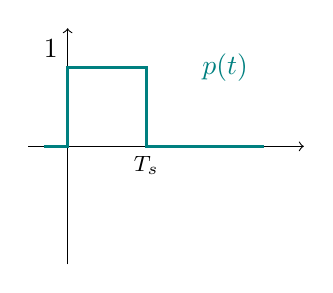
\begin{tikzpicture}
                \draw [->] (-0.5,0) -- (3,0);
                \draw [->] (0,-1.5) -- (0,1.5);                               \node at (0,1) [anchor=south east] {$1$}; 
                \draw[very thick, teal] (-.3,0) -- (0,0) -- (0,1) -- (1,1) -- (1,0) -- (2.5,0);
                \node at (1,0) [below] {\footnotesize $T_s$}; 
                \node at (2,1) [teal,] {$p(t)$}; 
            \end{tikzpicture} \hspace{1cm}
            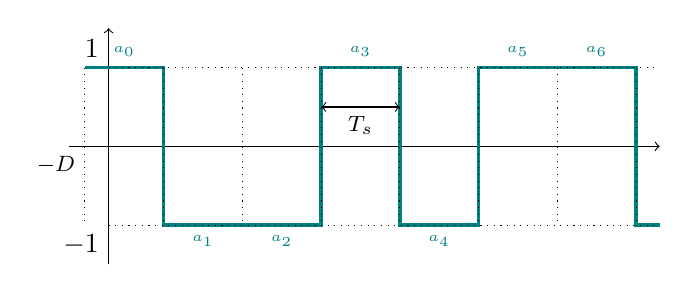
\begin{tikzpicture}
                \draw [->] (-0.5,0) -- (7,0);
                \draw [->] (0,-1.5) -- (0,1.5);
                \node at (0,1) [anchor=south east] {$1$}; 
                \node at (0,-1) [anchor=north east] {$-1$};
                \node at (-.3,0) [anchor=north east] {\footnotesize $-D$};
                \draw[very thick, teal] (-.3,1) --node[midway,above] {\tiny $a_0$} (.7,1) -- (.7,-1) --node[midway,below] {\tiny $a_1$} (1.7,-1) --node[midway,below] {\tiny $a_2$} (2.7,-1)-- (2.7,1) --node[midway,above] {\tiny $a_3$} (3.7,1) -- (3.7,-1) --node[midway,below] {\tiny $a_4$} (4.7,-1) -- (4.7,1) --node[midway,above] {\tiny $a_5$} (5.7,1) --node[midway,above] {\tiny $a_6$} (6.7,1) -- (6.7,-1) -- (7,-1);
                \draw [dotted,thin] (0,1) -- (7,1);
                \draw [dotted,thin] (0,-1) -- (7,-1);
                \foreach \x in {0,1,2,3,4,5,6,7} {
                  \draw [dotted,thin] (\x-.3,1) -- (\x-.3,-1);
                }

                \draw[<->] (2.7,.5) --node[midway,below] {\footnotesize $T_s$} (3.7,.5);
            \end{tikzpicture}
        \end{center}
        \caption{Pulso base y realización de una onda binaria aleatoria del Ejemplo \ref{ej:onda binaria aleatoria}.}\label{fig:onda binaria aleatoria}
    \end{figure}

    Calculemos media y autocorrelación de este proceso. Comenzamos por la media: para ello condicionamos a un valor de $D=z$ y luego integramos entre todos los posibles valores de esta variable uniforme, quedando:
    \begin{equation*}
        \E{x(t)} = \int_0^{T_s} \E{x(t)\mid D=z} \frac{1}{T_s} dz.
    \end{equation*}
    Ahora, dado $D=z$, observemos que:
    \begin{equation*}
        p(t-kT_s + z) = 1 \iff 0\leqslant t-kT_s +z < T_s \iff k\leqslant \frac{t + z}{T_s} < k+1.
    \end{equation*}
    Es decir, existe un único $k=k_0 = \left\lfloor \frac{t+z}{T_s}\right\rfloor$ tal que $p(t-k_0T_s + z) = 1$. Básicamente esto ocurre porque los pulsos no se solapan y por lo tanto en cada momento del tiempo $t$ observamos un único símbolo $a_k$. Entonces:
    \begin{equation*}
        \E{x(t)\mid D =  z} = P(a_{k_0} = 1) (1) + P(a_{k_0} = -1) (-1) = \frac{1}{2}-\frac{1}{2} = 0, 
    \end{equation*}
    de donde $\mu = \E{x(t)} = 0$ para todo $t$, es decir la señal tiene media constante y no tiene componente de continua.

    Pasemos ahora a calcular la correlación $R(t_1,t_2) = \E{x(t_1)x(t_2)}$.    Distinguimos dos casos:
    \begin{enumerate}
        \item Si $|t_1-t_2|>T_s$, entonces los símbolos observados en $t_1$ y $t_2$ son independientes, ya que pertenecen a pulsos distintos. Es decir, existen $k_1\neq k_2$ como antes, tales que $p(t_1-k_1T_s+z) = 1$ y $p(t_2-k_2T_s+z) = 1$. En ese caso:
        \begin{equation*}
          \E{x(t_1)x(t_2)\mid D=z} = \E{a_{k_1}a_{k_2}} = \E{a_{k_1}}\E{a_{k_2}} = 0,  
        \end{equation*}
        es decir no hay correlación para $|t_2-t_1|\geqslant T_s$, a distancia más de un tiempo de símbolo.

        \item Si en cambio $|t_2-t_1|<T_s$, entonces los símbolos pueden corresponder al mismo pulso, o a pulsos consecutivos, dependiendo de la fase. Supongamos primero que $t_2>t_1$ y que $x(t_1)=a_k$. La observación crucial es que el tiempo de cambio de símbolo $T_{k+1}$ tiene distribución uniforme en $[t_1,t_1+T_s]$, por lo que:
        \begin{equation*}
            \begin{cases}
            x(t_1) = x(t_2) = a_k \quad  \text{Si } t_2-t_1 < T_{k+1}, \\
            x(t_1) = a_k, x(t_2) = a_{k+1} \quad  \text{Si } t_2-t_1 \geqslant T_{k+1}.
            \end{cases}
        \end{equation*}
        Por lo tanto:
        \begin{align*}
            \E{x(t_1)x(t_2)} &= \overbrace{\E{a_k^2}}^{=1} \p{T_{k+1}>t_2-t_1} + \overbrace{\E{a_ka_{k+1}}}^{=0}\p{T_{k+1}\leqslant t_2-t_1} \\
            &= 1-\frac{(t_2-t_1)}{T_s}. 
        \end{align*}
    \end{enumerate}

    Un razonamiento análogo para $t_2<t_1$ permite concluir que el proceso es WSS (la autocorrelación solo depende de $\tau=t_2-t_1$) y su función de autocorrelación es:
    \begin{equation}\label{eq:autocorrelacion onda binaria centrada}
        R_x(\tau) = 1-\frac{|\tau|}{T_s} \quad -T_s\leqslant \tau \leqslant T_s,
    \end{equation}
    y $0$ en otro caso.

    \begin{center}
        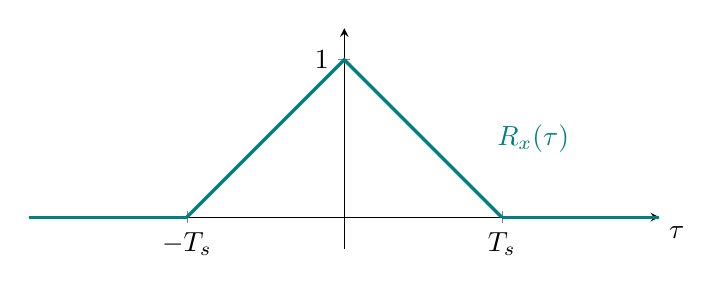
\begin{tikzpicture}
            \begin{axis}[ x=2cm, y=2cm, axis lines=middle,  
                        xlabel=$\tau$,
                        x label style={anchor=north west},
                        xmin=-2,xmax=2,ymin=-.2,ymax=1.2,
                        ytick={1},
                        xtick = {-1,1},
                        xticklabels = {$-T_s$,$T_s$},
                        clip=false,
                        ]
            \addplot [domain=-1:1, teal, very thick, samples=11] {1-abs(x)}; 
            \addplot [domain=-2:-1, teal, very thick, samples=2] {0}; 
            \addplot [domain=1:2, teal, very thick, samples=2] {0}; 
            \node[teal] at (axis cs: 1.2,.5) {$R_x(\tau)$};
            \end{axis}
        \end{tikzpicture}
    \end{center}
\end{ejemplo}





\begin{definicion}[Proceso Gaussiano]
    
\end{definicion}

\begin{definicion}[Ruido blanco Gaussiano (WGN)]
    
\end{definicion}
%\section{Ruido y modelos determinísticos}

Denominamos ``ruido"  en un sistema de comunicaciones a una señal
que se superpone a las de interés, originada en diversas cuasas,
por ejemplo:

    \begin{itemize}
        \item agitación térmica
        \item llaves que conmutan
        \item interferencia de otros canales
    \end{itemize}
Características:
    \begin{itemize}
        \item impredecible
        \item persistente
        \item aperiódico
    \end{itemize}

\begin{figure}[htb]
    \centering\begin{minipage}{0.8\textwidth}
    \bpgf{Imagenes/ruido/ruido-1}
    \begin{tikzpicture}
        \draw[-stealth]  (-0.5,0) -- (8,0) node [anchor=north] {$t$};
        \draw[-stealth] (0,-1) -- (0,3) node [anchor=west] {$x$};
        \draw [samples=50,domain=0:7] plot (\x,{cos(\x r)+(0.5*exp(\x*0.05)-exp(-\x*0.1))+0.3*rand});
    \end{tikzpicture}
    \endpgfgraphicnamed\end{minipage}
\end{figure}
\FloatBarrier

Al diseñar el sistema de comunicación no conocemos la forma de
onda, pero es posible conocer información ``en promedio''.

\paragraph{Dos posibles modelos: }$\phantom{1}$

\begin{minipage}[t]{0.45\textwidth}
    Determinístico, promedios en el tiempo

    \begin{align*}
        \text{Valor medio:}\  \langle x \rangle &= \lim_{T\to\infty} \frac{1}{T} \int^{\frac{T}{2}}_{-\frac{T}{2}} x(t)\d t\\
        \text{Potencia media:}\ \langle x^2 \rangle &= \lim_{T\to\infty} \frac{1}{T} \int^{\frac{T}{2}}_{-\frac{T}{2}} x^2(t)\d t
    \end{align*}
\end{minipage}
\hfil
\begin{minipage}[t]{0.45\textwidth}
    Proceso aleatorio $X(t,\alpha)$, promedios ``en el ensemble'', es decir en ``sorteo'' $\alpha$.
    \begin{align*}
        \text{Valor esperado:} &\quad E \left[X(t,\alpha)\right]\\
        \mbox{}\\
        \text{Momento de orden $2$:} &\quad E \left[X^2(t,\alpha)\right]
    \end{align*}
\end{minipage}

Nos interesa obtener información \emph{espectral} sobre este tipo
de señales, pese a no disponer de una fórmula sencilla para $x(t)$
y por tanto no disponer de una transformada de Fourier.


En ese sentido, comparemos una señal de ruido como $x(t)$ de la
figura anterior con otra, %$\tilde{x}(t)$

    \begin{figure}[htb]
    \centering\begin{minipage}{0.8\textwidth}
                \bpgf{Imagenes/ruido/ruido-2}
                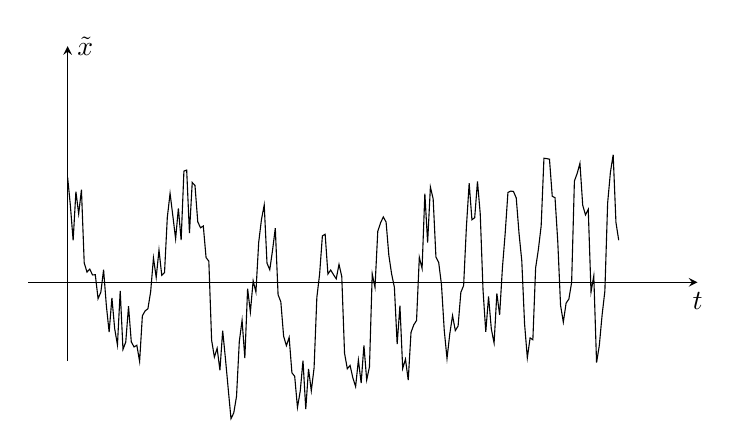
\begin{tikzpicture}
                \draw[-stealth]  (-0.5,0) -- (8,0) node [anchor=north] {$t$};
                \draw[-stealth] (0,-1) -- (0,3) node [anchor=west] {$\tilde{x}$};
                \draw [samples=200,domain=0:7] plot (\x,{cos((\x+1)^2 r)+0.5*cos(\x r)+0.5*rand});
            \end{tikzpicture}
                \endpgfgraphicnamed
             \end{minipage}
\end{figure}
\FloatBarrier

 Puede ocurrir que la potencia media sea igual en
ambas, es decir $\langle x^2\rangle = \langle \tilde{x}^2
\rangle$, pero su efecto en un sistema será en general diferente,
debido a que la segunda ``varía más rápido" en el tiempo. Por
ejemplo, a la salida de un pasabajos, $\tilde{x}$ se atenuará más,
su potencia está en ``frecuencias más altas¨. Queremos formalizar
este concepto pese a que no disponemos de una transformada de
Fourier de la propia señal.

El camino para el análisis es el estudio de la
\emph{autocorrelación} de la señal $r_x(\tau)$, y su transformada
de Fourier, la {\em densidad espectral de potencia} $S_x(f)$.
Repasamos ambos conceptos a continuación, comenzando por los
modelos determinísticos.

%
% Vemos que si bien
%tienen características bien distintas. Puede pasar que pero ambas
%no tienen el mismo efecto en un sistema. Por lo tanto importa
%poder decir cómo se distribuye esa potencia entre las distintas
%frecuencias. Esta información, la es crucial para el análisis del
%ruido.
%
%    No es fácil hallar $\hat{X}_2(f)$ para este tipo de señales. El camino para introducir $S_x(f)$ es a través de la  $x_2(t)$.


\subsection*{Modelo determinístico: señales de potencia finita}

\subsubsection*{Autocorrelación y densidad espectral de potencia}

\[r_x(\tau)=\lim_{T\rightarrow\infty} \frac{1}{T}\int^{\frac{T}{2}}_{-\frac{T}{2}} x(t)\overline{x(t-\tau)}\d t.\]

\begin{propiedadesSN}\mbox{}
    \begin{enumerate}
        \item $r_x(0)=\langle x^2\rangle$.
        \item $|r_x(\tau)|\leq r_x(0)$.
        \item $r_x(\tau) = r_x(-\tau)$ si $x(t)$ es real.
    \end{enumerate}
\end{propiedadesSN}

Un valor grande de $r_x(\tau)$ quiere decir que $x(t)$ ``tiende a
repetirse'' cada $\tau$ segundos. Entonces $r_x(\tau)$ tiene
información de tipo espectral, es decir revela las periodicidades
de la señal. Esto conduce a considerar su transformada de Fourier,

\[r_x(\tau)\stackrel{\mathcal{F}}{\longrightarrow} S_x(f)\qquad\text{densidad espectral de potencia.}\]


\begin{propiedadesSN}\mbox{}
    \begin{enumerate}
        \item $S_x(f)\geq 0$.
        \item $\langle x^2\rangle = \int^{\infty}_{-\infty} S_x(f)\d
        f$.
    \end{enumerate}
\end{propiedadesSN}

Nos dice como se distribuye la potencia en frecuencia.

\subsubsection*{Filtrado}
%
%\begin{figure}[htb]
%    \centering
%    \bpgf{Imagenes/ruido/ruido-3}
%    \begin{blockdiagram}
%        \matrix[row sep=5mm, column sep=10mm]{
%            \node[etiqueta] (inicio) {$x(t)$}; & \node[block] (filtro) {$\hat{H}(f)$} node [above=3mm] {FILTRO LTI}; & \node[etiqueta] (salida) {$y(t)$};\\
%        };
%        \draw [-stealth] (inicio) -- (filtro);
%        \draw [-stealth] (filtro) -- (salida);
%    \end{blockdiagram}
%    \endpgfgraphicnamed
%\end{figure}

Excitamos un sistema LTI, con respuesta impulsiva $h(t)$,
respuesta en frecuencia $\hat{H}(f)$, con una señal de potencia
finita $x(t)$.

\begin{figure}[h]
    \centering
\setlength{\unitlength}{0.00500in}
\begin{picture}(380,160)(140,40)
\put(220,40){\framebox(120,120){}} \put(80,100){\vector(1,0){140}}
\put(340,100){\vector(1,0){140}}
\put(0,90){\makebox(0,0)[lb]{\raisebox{0pt}[0pt][0pt]{\large $x(t)$}}}%
\put(240,90){\makebox(0,0)[lb]{\raisebox{0pt}[0pt][0pt]{\large $\hat{H}(f)$}}}%
\put(510,90){\makebox(0,0)[lb]{\raisebox{0pt}[0pt][0pt]{\large $y(t)$}}}%
\end{picture}
\end{figure}
\FloatBarrier

Se cumple:

\begin{align*}
r_y & =r_x\ast h \ast \tilde{h}\ \  \text{ donde } \ \
\tilde{h}(t)=h(-t) \\
\Rightarrow S_y(f)&=S_x(f)|\hat{H}(f)|^2.\end{align*}

\subsubsection*{Correlación y densidad espectral cruzada de dos señales}
\begin{align*}
    r_{xy}(\tau)&=\lim_{T\rightarrow\infty} \frac{1}{T}\int^{\frac{T}{2}}_{-\frac{T}{2}}x(t)\overline{y(t-\tau)}\d t.\\
    r_{xy}&=\overline{r_{yx}(-\tau)}.\\
    S_{xy}(f)&=\mathcal{F}\left[r_{xy}(\tau)\right] \text{ (no necesariamente positiva)}.\\
\end{align*}

Si $y(t)$ se obtiene de filtrar $x(t)$ como arriba:
\[ r_{xy} = r_x \ast \tilde{h},\qquad S_{xy}(f)=\overline{\hat{H}(f)} S_x(f).\]

\emph{Señales ``incoherentes'': } si $r_{xy}\equiv 0$. En ese
caso, $\langle (x+y)^2 \rangle = \langle x^2 \rangle + \langle y^2
\rangle$.

\subsubsection*{Ruido blanco}

Señal que cumple $S_n(f)\equiv \frac{\eta}{2}\,\forall\,f$. La potencia de salida de un filtro excitado por ruido blanco es
\[N=\frac{\eta}{2}\int^\infty_{-\infty}\left|\hat{H}(f)\right|^2\d f.\]

\subsection*{Aplicación: ruido en la comunicación de banda base}

\begin{figure}[htb]
    \centering\begin{minipage}{\textwidth}
    \bpgf{Imagenes/ruido/ruido-4}
    \begin{blockdiagram}
        \matrix[row sep=5mm, column sep=10mm]{
        & & \node [etiqueta] (ruido) {$n(t)$}; &\\
        \node [etiqueta] (inicio) {$x(t)$}; & \node [block] (canal) {CANAL}; & \node [operator] (sum) {$+$}; & \node [etiqueta] (salida) {$x_R(t)$};\\
        };
        \draw [-stealth] (inicio) -- (canal);
        \draw [-stealth] (canal) -- (sum);
        \draw [-stealth] (ruido) -- (sum);
        \draw [-stealth] (sum) -- (salida);
    \end{blockdiagram}
    \endpgfgraphicnamed\end{minipage}
\end{figure}
\FloatBarrier

\paragraph{Suponemos: }
\begin{itemize}
    \item $x(t)$ señal de banda acotada a $B$, potencia $\langle x^2
    \rangle$.
    \item $x_R(t) = Kx(t) + n(t)$, $n(t)$ ruido blanco,
    $S_n(f)=\frac{\eta}{2}$.
\end{itemize}

Si comparamos potencias, la señal está sumergida en ruido (de
potencia infinita!) Para mejorar las cosas agregamos un filtro
pasabajos de ancho $B$.


\begin{figure}[htb]
    \centering\begin{minipage}{\textwidth}
    \bpgf{Imagenes/ruido/ruido-3}
    \begin{blockdiagram}
        \matrix[row sep=5mm, column sep=10mm]{
            \node[etiqueta] (inicio) {$x_R(t)$ \quad }; & \node[block] (filtro) {PASABAJOS $B$}; & \node[etiqueta] (salida) {\quad $x_D(t)+n_D(t)$};\\
        };
        \draw [-stealth] (inicio) -- (filtro);
        \draw [-stealth] (filtro) -- (salida);
    \end{blockdiagram}
    \endpgfgraphicnamed\end{minipage}
\end{figure}



%
%\begin{figure}[h]
%    \centering
%\setlength{\unitlength}{0.00500in}
%\begin{picture}(380,160)(140,40)
%\put(220,40){\framebox(120,120){}} \put(80,100){\vector(1,0){140}}
%\put(340,100){\vector(1,0){140}}
%\put(-20,90){\makebox(0,0)[lb]{\raisebox{0pt}[0pt][0pt]{ $x_R(t)$}}}%
%\put(230,90){\makebox(0,0)[lb]{\raisebox{0pt}[0pt][0pt]{ $\hat{H}(f)$}}}%
%\put(510,90){\makebox(0,0)[lb]{\raisebox{0pt}[0pt][0pt]{ $x_D(t)+n_D(t)$}}}%
%\end{picture}
%\end{figure}
%\FloatBarrier

A la salida tenemos $x_D(t)=Kx(t)$ y un ruido $n_D(t)$ de potencia
media
\[\langle n_D^2 \rangle = \int^\infty_{-\infty} S_{n_D}(f)\d f =
\frac{\eta}{2}\int^\infty_{-\infty}\left|\bar{H}(f)\right|^2\d f=
\eta B.\]

Por lo tanto, relación señal - ruido a la salida es
\[
\left(\frac{S}{N}\right)_D= \dfrac{K^2\langle x^2 \rangle}{\eta
B}.\]

%\section{Procesos aleatorios estacionarios}\label{sec.estoc}

\begin{figure}[h]
    \centering\begin{minipage}{\textwidth}
    \bpgf{Imagenes/estoc/estoc-1}
    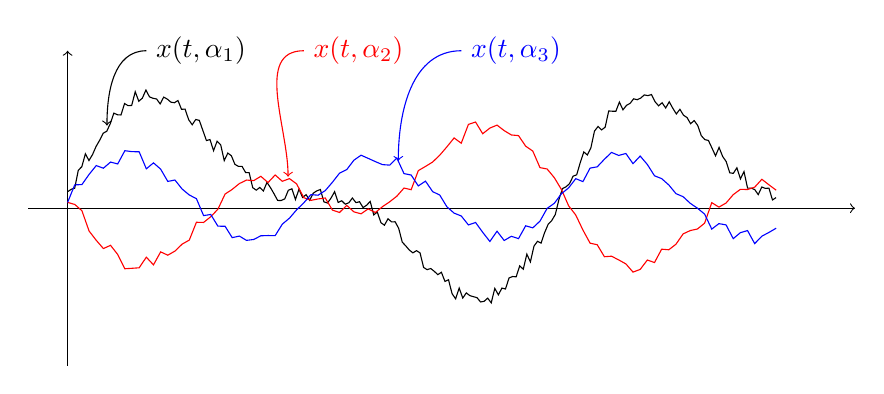
\begin{tikzpicture}
        \draw [->] (-0.5,0) -- (10,0);
        \draw [->] (0,-2) -- (0,2);
        \draw [samples=200,domain=0:9] plot (\x,{0.15+sin(\x r)*(1+cos(\x r +1))+0.1*rand});
        \draw [->] (1,2) node [anchor=west] {$x(t,\alpha_1)$} to [out=180,in = 90] (0.5,1.05);
        \draw [samples=100,domain=0:9,color=red] plot (\x, {0.15-sin(\x r)*(0.5+cos(\x r +1))+0.1*rand});
        \draw [->,color=red] (3,2) node [anchor=west,color=red] {$x(t,\alpha_2)$} to [out=180,in=90] (2.8,0.4);
        \draw [samples=100,domain=0:9,color=blue] plot (\x, {0.15+sin(\x r)*(cos(\x r +1))+0.1*rand});
        \draw [->,color=blue] (5,2) node [anchor=west,color=blue] {$x(t,\alpha_3)$} to [out=180,in=90] (4.2,0.6);
    \end{tikzpicture}
    \endpgfgraphicnamed\end{minipage}
    \end{figure}

Sorteo una señal a través de $\alpha\in\Omega$, espacio de probabilidad.
\begin{itemize}
    \item Para cada sorteo $\alpha$ tengo una {\em trayectoria}
    $X(t,\alpha)$.
    \item Para cada $t$ tengo una variable aleatoria $X(t)$. En particular, tiene una distribución de probabilidad $F_{X(t)}(x)$ y puedo calcular
    momentos $E\left[X(t)\right]$, $E\left[X^2(t)\right]$: promedios en el ``ensemble'', para $t$ fijo.
\end{itemize}

La familia de distribuciones \emph{conjuntas} de las variables
aleatorias $X(t_1),\ldots,X(t_n)$ para cualesquiera tiempos
$(t_1,t_2,\ldots,t_n)$ caracteriza al proceso.

En general la distribuci\'on del proceso puede variar en el
tiempo. Un proceso se dice {\bf estrictamente estacionario} si
esto no ocurre, es decir que la distribución de
$\left(X(t_1),\ldots,X(t_n)\right)$ es igual a la de
$\left(X(t_1+\tau),\ldots,X(t_n+\tau)\right)$ para cualquier
$\tau$.

Se trabaja en general una noción más amplia de proceso
estacionario, a definirse a continuación. Notamos que cualquier
proceso estrictamente estacionario con momento de segundo orden
finito cumple también la definición que sigue.

\subsection*{Proceso estacionario (sentido amplio)}
Un proceso aleatorio $X(t)$ es estacionario en sentido amplio si
se cumple:
\begin{enumerate}
    \item $E\left[X(t)\right]=\mu$, constante en el tiempo.
    \item $E\left[X(t)X(t-\tau)\right]=R_X(\tau)$ (autocorrelación en sentido aleatorio) independiente de $t$.
\end{enumerate}

\newpage

{\bf Ejemplo 1: Sinusoide de fase aleatoria.}

%\begin{ejemplo}[Sinusoide de fase aleatoria]$\phantom{1}$

$X(t)=\cos(\omega_0t+\theta)$, con $\theta$ variable aleatoria de
distribución uniforme en $[0,2\pi]$. Esto modela una señal
sinusoidal con frecuencia conocida pero de la que no tenemos
información de sincronismo.

\begin{align*}
    E\left[X(t)X(t-\tau)\right]     & = E\left[\cos(\omega_0t+\theta)\cos\left(\omega_0(t-\tau)+\theta\right)\right]\\
                    & = E\left[\frac{\cos(\omega_0\tau)}{2}+\frac{\cos(2\omega_0t-\omega_0\tau+2\theta)}{2}\right]\\
                    & = \frac{1}{2}\cos(\omega_0\tau)+\frac{1}{2\pi}\int_0^{2\pi}\frac{\cos(2\omega_0t-\omega_0\tau+2\theta)}{2}\d\theta\\
                    & = \frac{1}{2}\cos(\omega_0\tau).
\end{align*}
Por lo tanto $R_X(\tau)=\frac{1}{2}\cos(\omega_0\tau)$. Por un
cálculo similar tenemos que $E\left[X(t)\right]=0$, y por lo tanto
el proceso es estacionario en sentido amplio.
%\end{ejemplo}

%\begin{ejemplo}[Onda binaria aleatoria] $\phantom{1}$

{\bf Ejemplo 2: Onda binaria aleatoria} \\

    \begin{minipage}{0.65\textwidth}
        \resizebox{\textwidth}{!}{
        \bpgf{Imagenes/estoc/estoc-2}
        \begin{tikzpicture}
            \draw [->] (-0.5,0) -- (7,0);
            \draw [->] (0,-1.5) -- (0,1.5);
            \path (0,1) node [anchor=east] {$1$} -- (0,-1) node [anchor=east] {$-1$};
            \draw (0,1) -- (1,1) -- (1,-1) -- (3,-1) -- (3,1) -- (4,1) -- (4,-1) -- (5,-1) -- (5,1) -- (6.5,1);
            \path (1,0) node [anchor=north west] {$T$};
            \draw [dotted,thin] (2,0) node [anchor=south] {$2T$} -- (2,-1);
        \end{tikzpicture}
        \endpgfgraphicnamed
        }
    \end{minipage}
    \hfill
    \begin{minipage}{0.3\textwidth}
        $X(t)=X_k$ constante en $[kT,(k+1)T)$;

        $\lbrace X_k\rbrace$ sucesión de V.A. independientes,
        distribuidas en $\pm 1$ con probabilidad $\frac{1}{2}$.
    \end{minipage}

    \noindent Es facil ver que $E\left[X(t)\right]=0$. ¿$X(t)$ es estacionario? No, los instantes $\lbrace kT\rbrace$ son ``especiales''. En
    particular, $E\left[X(t)X(t-\tau)\right]$ va a depender no
    sólo de $\tau$, sino también de si hay o no una frontera de
    intervalo $kT$ entre estos tiempos. Por ejemplo:
    \begin{gather*}
        X\left(\tfrac{T}{4}\right)=X\left(\tfrac{3T}{4}\right)\ \ \text{con probabilidad $1$, pero
        } \
        P\left(X\left(\tfrac{3T}{4}\right)=X\left(\tfrac{5T}{4}\right)\right)=\frac{1}{2},
    \end{gather*}
de donde se deduce que $E\left[X(t)X(t-\frac{T}{2})\right]$ vale
$1$ para $t=\frac{3}{4}$, y vale $0$ para
    $t=\frac{5}{4}$. O sea que no tenemos una autcorrelación
    dependiente solo de $\tau$.

    Una forma de definir una onda binaria aleatoria estacionaria es agregar un retardo aleatorio
    $D$, uniforme en $[0,T]$, e independiente de $X(t)$.
    Intuitivamente, esto quita el sincronismo de los instantes
    $kT$ y ``todos los tiempos se vuelven iguales".

    Formalmente, sea $Y(t)=X(t-D)$. Este proceso es constante,
    igual a $X_k$ en el intervalo $[kT+D,(k+1)T+D)$.
Fijados dos tiempos, $t-\tau$, $t$ sea ``$A$" el
    suceso ``ambos tiempos caen en el mismo intervalo (mismo
    $k$)". Como la distribución de $D$ es uniforme en $[0,T]$, la probabilidad de
    $A$ decrece linealmente con $\tau$ hasta $\tau = T$, donde
    se vuelve nula. Es decir
    \[P(A) = \begin{cases}
                1-\frac{|\tau|}{T} & 0\leq |\tau|\leq T,\\
                0 & |\tau|>T.
            \end{cases}\]
Calculamos $E[Y(t)Y(t-\tau)]$, utilizando la probabilidad
condicional a los sucesos $A$ y su complemento $A^c$. Si ocurre
$A$, $Y(t)=Y(t-\tau)=\pm 1$ por tanto el valor esperado
condicional es  $E[Y(t)Y(t-\tau)|A]= 1$. Si en cambio ocurre
$A^c$, $Y(t)$, $ Y(t-\tau)$ son independientes y el valor esperado
es cero. Combinandolos
\begin{align*}
E[Y(t)Y(t-\tau)] & = E[Y(t)Y(t-\tau)|A] \cdot P(A) +
E[Y(t)Y(t-\tau)|A^c]\cdot P(A^c) \\
& = 1\cdot P(A)+0\cdot P(A^c)\\
&= P(A).
\end{align*}
Como $P(A)$ depende sólo de $\tau$, $Y(t)$ es estacionario con
autocorrelación \[ R_Y(\tau)=\begin{cases}
                1-\frac{|\tau|}{T} & 0\leq |\tau|\leq T,\\
                0 & |\tau|>T.
            \end{cases}\]

\subsection*{Relación entre correlaciones temporales y probabilísticas}

Para un proceso estacionario tenemos entonces dos definiciones de
autocorrelación:
\begin{itemize}
    \item La aleatoria $R_X(\tau)=E[X(t)X(t-\tau)]$.
    \item En cada trayectoria $x(t)= X(t,\alpha)$ (cada resultado del sorteo), podemos calcular la autocorrelación determinística
    $r_x(\tau) = \lim_{T\rightarrow\infty} \frac{1}{T}\int^{\frac{T}{2}}_{-\frac{T}{2}}
    x(t)x(t-\tau)\d t.$
\end{itemize}
En principio, la segunda podría depender de $\alpha$ (el sorteo),
y no tendría por qué coincidir con la primera. Sin embargo, en una
clase importante de procesos, llamados \emph{ergódicos}, se
verifica la igualdad de las medias temporales y probabilísticas.
%
%%\paragraph{Preguntas:}
%\begin{itemize}
%    \item ¿La segunda depende de?
%    \item ¿Son iguales?
%\end{itemize}
%
%Este concepto, iguadad de medias temporales y probabilísticas se
%llama  del proceso.

\paragraph{Recordar:} ``Ley de los grandes números'' en probabilidad.

Dado $X_1,X_2,\ldots,X_k,\ldots$ sucesión de V.A. independientes,
idénticamente distribuidas (I.I.D.), con $E[X_k]=\mu$. Entonces
con probabilidad $1$,
\[\frac{X_1+X_2+\cdots+X_k}{k}\xrightarrow[k\rightarrow\infty]{}\mu.\]

Promedio temporal $=$ promedio probabilístico.

Esto es un ejemplo de \emph{ergodicidad} (en la media). Vale para
variables independientes, o en aquellas en que la dependencia se
``apaga'' al alejarnos en el tiempo.

\paragraph{Versión de tiempo continuo:} $X(t)$  ergódico en el media si
\[\lim_{T\rightarrow\infty}\frac{1}{T}\int^{\frac{T}{2}}_{-\frac{T}{2}}X(t)\d t \underset{\text{con prob $1$}}{=}E\left[X(t)\right].\]

$X(t)$ ergódico en el autocorrelación si:
\[\lim_{T\rightarrow\infty}\frac{1}{T}\int^{\frac{T}{2}}_{-\frac{T}{2}}X(t)X(t-\tau)\d t \underset{\text{con prob $1$}}{=}E\left[X(t)X(t-\tau)\right].\]
En otras palabras $R_X(\tau)=r_X(\tau)$ con probabilidad 1.

Intuitivamente, en un proceso ergódico la trayectoria de
$X(t,\alpha)$ toma a lo largo del tiempo valores representativos
de la distribución, de modo que los promedios temporales
reconstruyen el promedio en todos los posibles sorteos.

En adelante, supondremos que todos los procesos estacionarios que
encontraremos son ergódicos. Los promedios en el tiempo y en la
muestra coinciden.

\subsection*{Densidad espectral de potencia de un proceso ergódico}

Si se cumple la identidad $R_X(\tau)=r_X(\tau)$, podemos utilizar
la transformada de Fourier de la primera para calcular la densidad
espectral de potencia de las trayectorias del proceso. Lo hacemos
en los ejemplos anteriores:


\begin{enumerate}
    \item Sinusoide de fase aleatoria, $\cos(\omega_0t+\theta)$.
    \[R_X(\tau)=\frac{1}{2}\cos(\omega_0\tau)\Rightarrow S_X(f)=\frac{\delta(f+f_0)+\delta(f-f_0)}{4}.\]

    \paragraph{Nota: } el mismo resultado se obtiene para sinusoides determinísticas sin fase aleatoria. Esto no sorprende, ya que el cambio de fase no afecta la autocorrelación.

    \item Onda binaria aleatoria con retardo uniforme
    \[R_Y(\tau)=1-\frac{|\tau|}{T} \ \ \mbox{ para } |\tau|\leq T \quad \Rightarrow S_Y(f) = T\left[\sinc^2(\pi f T)\right].\]
    Esto nos dice donde se distribuye la potencia de una onda
    digital, lo cual sería difícil de obtener sin recurrir a la
    ergodicidad.
    \paragraph{Nota: } sin  el retardo aleatorio el proceso deja de ser estacionario, no puedo hallar $R_X(\tau)$.
    Pero en cada trayectoria, el retardo no afecta $r_x$, por lo tanto se puede argumentar que la densidad espectral de
    potencia calculada vale para la onda binaria sin retardo.
    \end{enumerate}

\subsection*{Procesos Gaussianos}

Un proceso es Gaussiano si las distribuciones conjuntas de
$\left(X(t_1),\ldots,X(t_n)\right)$ son normales (multivariadas)
para cualesquiera $t_1,\ldots,t_n$.  En particular, para cada $t$
$X(t)$ es una variable aleatoria normal, de densidad
$f_X(x)=\frac{1}{\sqrt{2\pi}\sigma}\e^{-\frac{(x-\mu)^2}{2\sigma^2}}$.

\noindent {\bf Propiedad:} una operación lineal (en particular,
filtrado) aplicada a un proceso Gaussiano da un resultado
Gaussiano.



\noindent {\bf Ejemplo:}
    \begin{figure}[htb]
        \centering\begin{minipage}{\textwidth}
        \bpgf{Imagenes/estoc/estoc-3}
        \begin{blockdiagram}
            \matrix[row sep=5mm, column sep=10mm]{
                \node[etiqueta] (inicio) {\begin{minipage}{5cm}
                                            Ruido blanco, Gaussiano, media $0$, densidad espectral de potencia $\frac{\eta}{2}$
                                          \end{minipage}}; & \node [block] (filtro) {PASABAJOS $B$}; & \node[etiqueta] (final) {\quad $n(t)$};\\
            };
            \draw[->] (inicio) -- (filtro);
            \draw[->] (filtro) -- (final);
        \end{blockdiagram}
        \endpgfgraphicnamed\end{minipage}
    \end{figure}
    \FloatBarrier
\paragraph{Pregunta} ¿Cuál es la probabilidad de que $n(t)>K$?

Primero, observamos que  $n(t)$ es un proceso estacionario de
densidad espectral de potencia
$S_n(f)=\frac{\eta}{2}\left|\hat{H}(f)\right|^2$, donde
$\hat{H}(f)$ es la transferencia del pasabajos.  Suponemos que es
ergódico. También es Gaussiano. Por lo tanto $n(t)$ tiene
distribución normal, con parámetros
\begin{align*}
    \mu&=0,\\
    %\begin{aligned}
        \sigma^2    & = E\left[x^2(t)\right]\\
                & = R_X(0)\\
                & = \frac{\eta}{2}\int_{-\infty}^\infty
                \left|\hat{H}(f)\right|^2\d f \\
                & = \eta B.
    \end{align*}
%\end{gather*}
Esto permite calcular la probabilidad deseada:
\begin{align*}
P\left(n(t)>K\right) & = %\int_K^\infty f_n(x)\d x =
\frac{1}{\sqrt{2\pi}\sigma}\int_K^\infty
\e^{-\frac{x^2}{2\sigma^2}}\d x =
\frac{1}{\sqrt{2\pi}}\int_{\frac{K}{\sigma}}^\infty
\e^{-\frac{z^2}{2}}\d z = Q\left(\frac{K}{\sigma}\right)=
Q\left(\frac{K}{\sqrt{\eta B}}\right),
\end{align*}
donde \[ Q(x) = 1 - F_X(x) \] es la ``cola" de la distribución
normal $(0,1)$. Volveremos a esto en más detalle al estudiar
detección digital.

%\section{Modulación y procesos estacionarios}\label{sec.modest}

Sea $x(t)$, proceso estacionario con autocorrelación $R_x(\tau)$,
densidad espectral de potencia $S_x(f)$. Para esta sección suponemos también que
el valor medio $E[x(t)]=0$.

Nos interesa estudiar la
señal modulada $x(t)\cos(\omega_ct)$ con los mismas técnicas. Sin
embargo, este proceso no es estacionario, ya que se anula en
momentos fijos del tiempo. ?`Cómo proceder entonces?
Estudiamos dos alternativas.

%\subsection*{1. Introducir una fase aleatoria}
\begin{enumerate}
\item Modular con fase aleatoria.

Como ya se vio, una sinusoide de fase aleatoria uniforme es un proceso estacionario. Definimos entonces
\[z(t)=x(t)\cos(\omega_ct+\theta),\qquad \theta\sim U[0,2\pi],\text{ indep de }x(t).\]
Usando la independencia, se ve que $z(t)$ es un proceso estacionario cuya autocorrelación es el
producto de las autocorrelaciones de $x(t)$ y del coseno de fase
aleatoria:
\begin{align*}
    R_z(\tau)&=E\left[x(t)\cos(\omega_ct+\theta)x(t-\tau)\cos(\omega_ct+\theta-\omega_c\tau)\right]
    \\ & = R_x(\tau)E\left[\cos(\omega_ct+\theta)\cos(\omega_ct+\theta-\omega_c\tau)\right]
    \\ &=\frac{1}{2}R_x(\tau)\cos(\omega_c\tau).
\end{align*}
La correspondiente densidad espectral de potencia es
\[
 S_z(f) =\frac{S_x(f-f_c)+S_x(f+f_c)}{4}.
\]
Este modelo puede ser útil para estudiar situaciones en que no hay sincronismo entre la portadora y el proceso que modula.

\item Introducir una componente en cuadratura.

Complementamos aquí $x(t)$ con otro proceso $y(t)$ ``en
cuadratura",  y consideramos el proceso con envolvente compleja
$x(t) + j y(t)$, es decir
\[
u(t)=x(t)\cos(\omega_ct)  -y(t)\sen(\omega_ct).\]

Suponemos que $y(t)$ es un proceso aleatorio estacionario de iguales características que
$x(t)$, en particular de media 0 y $R_y(\tau)=R_x(\tau)$. Suponemos inicialmente que ambos procesos son
\emph{incoherentes}, es decir
\[
R_{xy} (\tau) = E[x(t)y(t-\tau)] \equiv 0.\]
En ese caso tendremos
\begin{align*}
                E\left[u(t)u(t-\tau)\right]  = &
                \ R_x(\tau)\cos(\omega_ct)\cos\left(\omega_c(t-\tau)\right)
                                 + R_y(\tau)\sen(\omega_ct)\sen\left(\omega_c(t-\tau)\right) \\
                                 = & \ R_x(\tau)\cos(\omega_c\tau),
            \end{align*}
en el que se utilizó para el último paso una identidad trigonométrica. Concluimos entonces que
el proceso $u(t)$ es estacionario, con densidad espectral de potencia
\[
S_u(f)=\frac{S_x(f-f_c)+S_x(f+f_c)}{2}.
\]
El hecho que $S_u(f)=2 S_z(f)$ se explica intuitivamente porque a través del proceso $y(t)$ se introdujo
``el doble de ruido".

De hecho, el procedimiento anterior puede generalizarse al caso en que $y(t)$ tenga correlación cruzada no nula
$R_{xy}(\tau)$, bajo cierta restricción, lo cual se aplica al estudio del ruido pasabanda que se verá a continuación.
Como esa generalización es algo técnica la incluimos en el Apéndice A al final de estas notas.
\end{enumerate}

%\section{Análisis del ruido pasabanda}\label{sec.ruidopasa}

Consideremos el ruido obtenido a la salida de un filtro pasabanda
de recepción:
\begin{figure}[htb]
    \centering%\begin{minipage}{\textwidth}
    \bpgf{Imagenes/ruidoPasa/ruidoPasa-1}
    \begin{blockdiagram}
        \matrix[row sep=5mm, column sep=10mm]{
             \node[punto] (inicio) {}; & \node[block] (filtro) {$[f_c-B,f_c+B]$}; & \node[etiqueta] (salida) {$\quad n(t)$};\\
        };
        \draw [->] (inicio) -- (filtro);
        \draw [->] (filtro) -- (salida);
    \end{blockdiagram}

    \endpgfgraphicnamed %\end{minipage}
\end{figure}
\FloatBarrier

$n(t)$ es estacionario, con densidad espectral de potencia
$S_n(f)$ que es de tipo pasabanda, es decir $S_n(f)=0$ fuera de la
banda $[f_c-B,f_c+B]$. Dentro de la banda, consideramos cualquier
densidad espectral, en particular no tiene por qué ser constante
en la banda ni simétrica respecto de $f_c$ (el filtro puede ser no
ideal, y/o el ruido de entrada no ser blanco). Suponemos que el
ruido es de media nula.

Para estudiar el efecto de dicho ruido en la demodulaci\'on, es conveniente tener una
representaci\'on de \emph{envolvente compleja} para el ruido:
$n_{ce}(t)=n_i(t)+jn_q(t)$ tal que
$n(t)=\Re\left[n_{ce}(t)\epi\right]$.
%
%\paragraph{Preguntas:} ¿Cómo definir $n_{ce}(t)$? ¿Es
%estacionario?

%
{\bf Preguntas:} ¿Cómo definir $n_{ce}(t)$? ¿Es estacionario?

Esta pregunta es en cierto sentido la inversa de la considerada en la secci\'on anterior.
All\'i se part\'ia de un proceso estacionario de banda base, y se buscaba un proceso modulado que tambi\'en fuese
estacionario. La respuesta tiene cierto grado de dificultad matem\'atica, por lo cual la diferimos para el Ap\'endice A.
Pero el resultado es afirmativo, lo indicamos en el siguiente enunciado:


\subsection*{Teorema}
Un proceso estacionario pasabanda $n(t)$, con densidad espectral
de potencia $S_n(f)$ concentrada en la banda
$|f|\in[f_c-B,f_c+B]$, puede escribirse como
\[n(t)=n_i(t)\cos(\omega_ct)-n_q(t)\sen(\omega_ct),\]
donde $n_i$, $n_q$ son procesos estacionarios pasabajos con igual
densidad espectral (concentrada en la banda $[-B,B]$):
\begin{center}
    \col{S_{n_i}(f)=S_{n_q}(f)=\underbrace{S_n(f-f_c)u\left(-(f-f_c)\right)}_{\oldstylenums{1}}+
    \underbrace{S_n(f+f_c)u(f+f_c)}_{\oldstylenums{2}}},
\end{center}
%
%\begin{gather*}
%    S_{n_i}(f)=S_n(f-f_c)u(f_c-f) + S_n(f+f_c)u(f+f_c),
%\end{gather*}
e igual potencia media  $E[n_i^2]=E[n_q^2]=E[n^2]$.

\noindent Además, si $S_n(f)$ es
simétrica respecto de $f_c$, entonces $n_i$, $n_q$ son incoherentes
(con correlaci\'on cruzada nula).



\paragraph{Representaci\'on gr\'afica:} Para interpretar la expresi\'on para la densidad espectral de
potencia de $n_i$, $n_q$, recurrimos al siguiente bosquejo:

\begin{figure}[htb]
    \centering\begin{minipage}{\textwidth}
    \bpgf{Imagenes/ruidoPasa/ruidoPasa-4}
        \begin{tikzpicture}
        \draw [->] (0,-6.5) -- (0,1.5) node [anchor=west] {$S_n(f)$};
        \draw [->] (-5,0) -- (5,0) node [anchor=north] {$f$};
        \begin{scope}[shift={(3,0)}]
            \draw (-1,0) .. controls (-0.5,0.3) and (-0.3,0.5) .. (0,0.5);
            \draw (0,0.5) .. controls (0.3,0.5) and (0.45,0.25) .. (0.5,0);
            \draw [dotted] (0,0) node [anchor=north] {$f_c$}--(0,0.5);
        \end{scope}

        \begin{scope}[shift={(-3,0)},xscale=-1]
            \draw (-1,0) .. controls (-0.5,0.3) and (-0.3,0.5) .. (0,0.5);
            \draw (0,0.5) .. controls (0.3,0.5) and (0.45,0.25) .. (0.5,0);
            \draw [dotted] (0,0) node [anchor=north] {$-f_c$} -- (0,0.5);
        \end{scope}

        \begin{scope}[shift={(0,-2)}]
            \draw [->] (-5,0) -- (5,0) node [anchor=north] {$f$};
            \begin{scope}[xscale=-1]
            \draw (-1,0) .. controls (-0.5,0.3) and (-0.3,0.5) .. (0,0.5);
            \draw (0,0.5) .. controls (0.3,0.5) and (0.45,0.25) .. (0.5,0);
            \end{scope}
            \path (0,0.5) node [anchor=south west] {$\oldstylenums{1}: S_n(f-f_c)u(f_c-f)$};
        \end{scope}

        \begin{scope}[shift={(0,-4)}]
            \draw [->] (-5,0) -- (5,0) node [anchor=north] {$f$};
            \draw (-1,0) .. controls (-0.5,0.3) and (-0.3,0.5) .. (0,0.5);
            \draw (0,0.5) .. controls (0.3,0.5) and (0.45,0.25) .. (0.5,0);
            \path (0,0.5) node [anchor=south west] {$\oldstylenums{2}: S_n(f+f_c)u(f+f_c)$};
        \end{scope}

        \begin{scope}[shift={(0,-6)}]
            \draw [->] (-5,0) -- (5,0) node [anchor=north] {$f$};
            \draw (-1,0) .. controls (-0.5,0.3) .. (-0.5,0.3);
            \draw (-0.5,0.3) .. controls (-0.35,0.75) and (-0.15,1) .. (0,1);
            \begin{scope}[xscale=-1]
            \draw (-1,0) .. controls (-0.5,0.25) .. (-0.5,0.3);
            \draw (-0.5,0.3) .. controls (-0.35,0.75) and (-0.15,1) .. (0,1);
            \end{scope}

            \path (1,1) node {$S_{n_i}(f)$};
        \end{scope}
    \end{tikzpicture}
    \endpgfgraphicnamed \end{minipage}
\end{figure}
\FloatBarrier
 Notar que se deduce del diagrama la identidad para la potencia total:
\[\langle{n_i^2}\rangle=E[n_i^2]
=\int S_{n_i}(f)\d f= \int \text{ \oldstylenums{1} }  + \int
\text{ \oldstylenums{2} } = \int S_n(f)\d f=E[n^2].\]



\paragraph{Nota:} Dados $n_i$, $n_q$ como arriba, para cualquier $\omega'_c$ la expresión
\[n'(t)=n_i(t)\cos(\omega'_ct)-n_q(t)\sen(\omega'_ct)\]
es siempre un proceso estacionario pasabanda, en la banda
$|f|\in[f'_c-B,f'_c+B]$.

Esto se deduce de lo visto en la secci\'on anterior para el
caso de $n_i$, $n_q$ incoherentes. Es también cierto en el caso general
(remitirse al Ap\'endice A).



\chapter{Modulación Digital en Banda Base}\label{chapter:modulacion banda base}

En este capítulo estudiaremos entonces el problema de enviar símbolos discretos a través de un medio analógico o canal. La Figura \ref{fig:mod_digital_bb} muestra el esquema básico de trabajo. El proceso de entrada es una secuencia de símbolos o proceso estocástico de tiempo discreto, $\{a_k:k\in\mathbb{Z}\}$, que asumiremos WSS y con valores en un alfabeto finito de tamaño $M$.

El sistema debe ser capaz de transmitir dichos símbolos por un canal físico (por ejemplo, par de cobre), utilizando una señal $x(t)$ \emph{que dependa de los símbolos a transmitir} y contenga la información. Dicha señal se verá afectada por el canal (atenuación, limitaciones de ancho de banda, ruido), por lo que la señal $\hat{x}(t)$ no es igual a la señal generada. Sin embargo, si muestreamos la señal en el momento correcto, puede ser posible decodificar el símbolo enviado con baja probabilidad de error.

En este capítulo analizaremos la llamada en \emph{modulación en banda base}, donde la secuencia de símbolos es codificada mediante una sucesión de \emph{pulsos analógicos} que duran un tiempo de símbolo, $T_s$. Como veremos, el pulso rectangular simple no siempre es la mejor opción. La razón por la que se denomina modulación es porque los símbolos digitales \emph{modulan} la secuencia de pulsos. La razón por la que se denomina en banda base es porque no intervienen componentes de alta frecuencia (ver Capítulo \ref{chapter:modulacion pasabanda}).

\begin{figure}[b]
    \begin{center}
        
        \begin{blockdiagram}[node distance=4em]
        \node [block,align=center] (fuente) {Fuente \\ digital};
        \node [block, right = of fuente] (tx) {Transmisor};
        \node [block, right= of tx] (ch) {Canal};
        \node [block, right = of ch] (rx) {Detector};
        \node [block, right = of rx, align=center] (sink) {Receptor \\ digital};

        \draw[thick, ->] (fuente)--node[midway,above] {$a_k$} (tx);
        \draw[thick, ->] (tx)--node[midway,above] {$x(t)$} (ch);
        \draw[thick, ->] (ch)--node[midway,above] {$\hat{x}(t)$} (rx);
        \draw[thick, ->] (rx)--node[midway,above] {$\hat{a}_k$} (sink);
        
        \node [block, below = 2em of ch] (sinc) {Sincronismo};
        \draw[thick, -] (tx) |- (sinc);
        \draw[thick, ->] (sinc) -| (rx);
        \end{blockdiagram}

        \caption{Esquema de un sistema de modulación digital.}\label{fig:mod_digital_bb}
    \end{center}
\end{figure}

Antes de continuar, definamos algunos parámetros relevantes a la hora de cuantificar la transferencia de información.

\begin{definicion}
    Definimos los siguientes parámetros:
    \begin{itemize}
        \item \emph{Velocidad de señalización} $f_s$. Es la frecuencia con la que se envía un símbolo, o bien $f_s=1/T_s$ siendo $T_s$ el tiempo de símbolo. Se mide en $\unit{baudios}:=\rfrac{\text{símbolos}}{\unit{\sec}}$.

    \item \emph{Velocidad de transmisión de información ($\vti$)}. Se mide en bits por segundo o $\unit{\bps}$. Si el alfabeto tiene $M$ símbolos, cada símbolo codifica $\log_2(M)$ bits de información, por lo que:
    \begin{equation*}
        \vti := f_s \log_2(M)
    \end{equation*}
    \item \emph{Ancho de banda del canal $B$} en $\unit{\Hz}$.
    \item \emph{Eficiencia espectral}:
     \begin{equation*}
        \mathrm{Eff} := \frac{\vti}{B},
     \end{equation*}
     y se mide en $\unit{\bps/\Hz}$.
    \end{itemize}
\end{definicion}
La $\vti$ es la velocidad que observa la capa superior. Por ejemplo, el estándar USB 1.1 permite hasta $1.5\unit{\mega\bps}$, mientras que el USB 2.0 lo eleva a $480 \unit{\mega\bps}$. Esa velocidad, como veremos, dependerá del ancho de banda físico $B$, la calidad del canal, así como de las formas de onda que representan los símbolos.

Los problemas que afectan a la transmisión por pulsos se muestran en la Figura \ref{fig:problemas canal}. El resultado final es un pulso distorsionado, pero que adecuadamente muestreado permite recuperar el símbolo transmitido.

\begin{figure}
    \begin{center}
    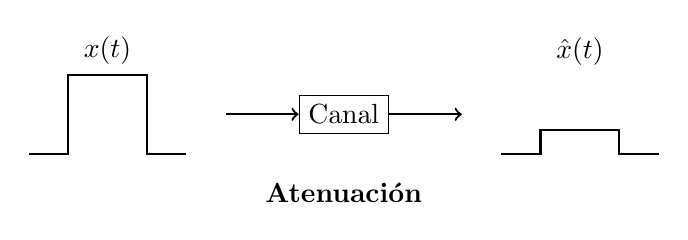
\begin{tikzpicture}
        \draw[thick] (1,0) -- (1.5,0) -- (1.5,1) --node[midway,above] {$x(t)$} (2.5,1) -- (2.5,0) -- (3,0);
        \node[rectangle,draw] at (5,0.5) (canal) {Canal};
        \draw[thick,->] (3.5,.5) -- (canal);
        \draw[thick,->] (canal) -- (6.5,.5);
        \draw[thick] (7,0) -- (7.5,0) -- (7.5,.3) -- (8.5,.3) -- (8.5,0) -- (9,0);
        \node[above] at (8,1) {$\hat{x}(t)$};
        \node at (5,-.5) {\textbf{Atenuación}};
    \end{tikzpicture}\hfill
    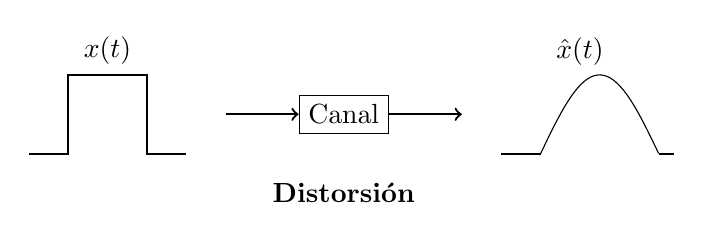
\begin{tikzpicture}
        \draw[thick] (1,0) -- (1.5,0) -- (1.5,1) --node[midway,above] {$x(t)$} (2.5,1) -- (2.5,0) -- (3,0);
        \node[rectangle,draw] at (5,0.5) (canal) {Canal};
        \draw[thick,->] (3.5,.5) -- (canal);
        \draw[thick,->] (canal) -- (6.5,.5);
        \draw[thick] (7,0) -- (7.5,0);
        \draw plot [thick,domain=7.5:9,samples=100] (\x,{sin(2*pi*(\x-7.5)/3 r)});
        \draw[thick] (9,0) -- (9.2,0);
        \node[above] at (8,1) {$\hat{x}(t)$};
        \node at (5,-.5) {\textbf{Distorsión}};
    \end{tikzpicture}
    \bigskip

    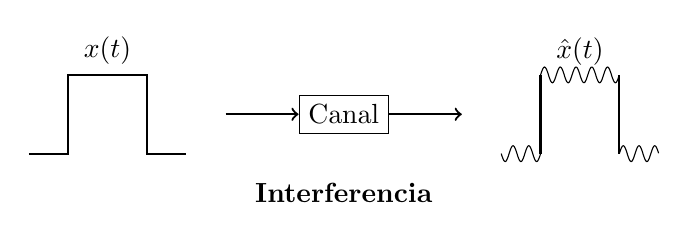
\begin{tikzpicture}
        \draw[thick] (1,0) -- (1.5,0) -- (1.5,1) --node[midway,above] {$x(t)$} (2.5,1) -- (2.5,0) -- (3,0);
        \node[rectangle,draw] at (5,0.5) (canal) {Canal};
        \draw[thick,->] (3.5,.5) -- (canal);
        \draw[thick,->] (canal) -- (6.5,.5);
        \draw plot [thick,domain=7:7.5,samples=100] (\x,{0.1*sin(2*5*pi*(\x-7.5) r)});
        \draw[thick] (7.5,0)--(7.5,1);
        \draw plot [thick,domain=7.5:8.5,samples=100] (\x,{1+0.1*sin(2*5*pi*(\x-7.5) r)});
        \draw plot [thick,domain=8.5:9,samples=100] (\x,{0.1*sin(2*5*pi*(\x-7.5) r)});
        \draw[thick] (8.5,1)--(8.5,0);
        \node[above] at (8,1) {$\hat{x}(t)$};
        \node at (5,-.5) {\textbf{Interferencia}};
    \end{tikzpicture}\hfill
    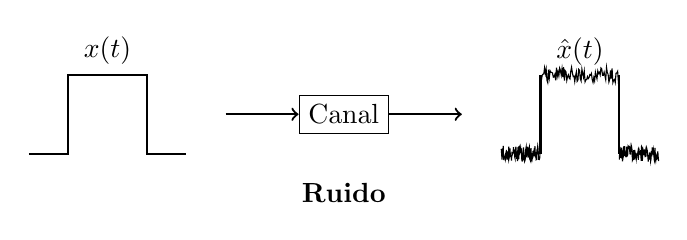
\begin{tikzpicture}
        \draw[thick] (1,0) -- (1.5,0) -- (1.5,1) --node[midway,above] {$x(t)$} (2.5,1) -- (2.5,0) -- (3,0);
        \node[rectangle,draw] at (5,0.5) (canal) {Canal};
        \draw[thick,->] (3.5,.5) -- (canal);
        \draw[thick,->] (canal) -- (6.5,.5);
        \draw plot [thick,domain=7:7.5,samples=100] (\x,.1*rand);
        \draw[thick] (7.5,0)--(7.5,1);
        \draw plot [thick,domain=7.5:8.5,samples=100] (\x,1+.1*rand);
        \draw plot [thick,domain=8.5:9,samples=100] (\x,.1*rand);
        \draw[thick] (8.5,1)--(8.5,0);
        \node[above] at (8,1) {$\hat{x}(t)$};
        \node at (5,-.5) {\textbf{Ruido}};
    \end{tikzpicture}
    \bigskip

    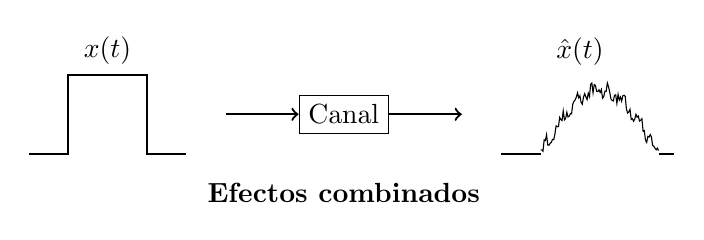
\begin{tikzpicture}
        \draw[thick] (1,0) -- (1.5,0) -- (1.5,1) --node[midway,above] {$x(t)$} (2.5,1) -- (2.5,0) -- (3,0);
        \node[rectangle,draw] at (5,0.5) (canal) {Canal};
        \draw[thick,->] (3.5,.5) -- (canal);
        \draw[thick,->] (canal) -- (6.5,.5);
        \draw[thick] (7,0) -- (7.5,0);
        \draw plot [thick,domain=7.5:9,samples=100] (\x,{0.8*sin(2*pi*(\x-7.5)/3 r)+ .08*rand + 0.05*sin(2*5*pi*(\x-7.5) r)});
        \draw[thick] (9,0) -- (9.2,0);
        \node[above] at (8,1) {$\hat{x}(t)$};
        \node at (5,-.5) {\textbf{Efectos combinados}};
    \end{tikzpicture}



    \caption{Problemas que afectan la transmisión por un canal.}\label{fig:problemas canal}
    \end{center}
\end{figure}

\section{Modulación por pulsos y codificación de línea}

El modelo básico de transmisión de datos en banda base es entonces la \emph{modulación por amplitud de pulsos (pulse amplitude modulation, PAM)}. En este caso, se tiene un proceso de símbolos $\{a_k:k\in\mathbb{Z}\}$ de $M$ símbolos, que interpretaremos como valores por ejemplo de voltaje o amplitud. Luego se eligen:
\begin{itemize}
    \item Un \emph{tiempo de símbolo} $T_s$ que corresponde luego a la frecuencia de señalización $f_s=1/T_s$.
    \item Una forma de pulso $p(t)$ (no necesariamente rectangular).
\end{itemize}

Para lograr la señalización se construye entonces la \emph{onda PAM}:
\begin{equation*}
    x(t) = \sum_{k} a_k p(t-kT_s),
\end{equation*}
es decir, cada símbolo se representa por un pulso de amplitud $a_k$ con origen en el tiempo $kT_s$ para el $k-$ésimo símbolo.

La elección combinada de las amplitudes posibles para $a_k$ y de la forma del pulso $p(t)$ determinan lo que se denomina \emph{codificación de línea}. En la Figura \ref{fig:codlin} se representan algunos códigos de línea utilizados en la práctica.

\begin{figure}
    \begin{center}
        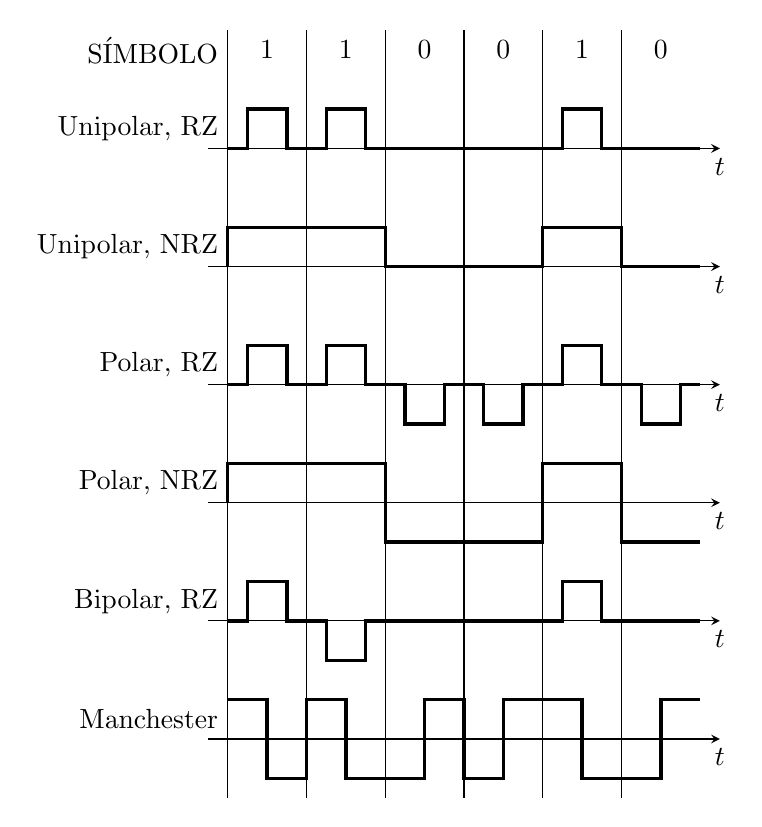
\begin{tikzpicture}[scale=0.5]
            \draw (0,1) -- (0,-18.5);
            \draw (2,1) -- (2,-18.5);
            \draw (4,1) -- (4,-18.5);
            \draw (6,1) -- (6,-18.5);
            \draw (8,1) -- (8,-18.5);
            \draw (10,1) -- (10,-18.5);
            \path (0,0.5) node [anchor=east] {SÍMBOLO} -- (1,0.5) node {$1$} -- (3,0.5) node {$1$} -- (5,0.5) node {$0$} -- (7,0.5) node {$0$} -- (9,0.5) node {$1$} -- (11,0.5) node {$0$};
            \begin{scope}[shift={(0,-2)}]
                \draw[-stealth] (-0.5,0) -- (12.5,0) node [anchor=north] {$t$};
                \path (0,0.5) node [anchor=east] {Unipolar, RZ};
                \draw[very thick] (0,0) -- (0.5,0) -- (0.5,1) -- (1.5,1) -- (1.5,0) -- (2.5,0) -- (2.5,1) -- (3.5,1) -- (3.5,0) -- (8.5,0) -- (8.5,1) -- (9.5,1) -- (9.5,0) -- (12,0);
            \end{scope}
            \begin{scope}[shift={(0,-5)}]
                \draw[-stealth] (-0.5,0) -- (12.5,0) node [anchor=north] {$t$};
                \path (0,0.5) node [anchor=east] {Unipolar, NRZ};
                \draw [very thick] (0,0) -- (0,1) -- (4,1) -- (4,0) -- (8,0) -- (8,1) -- (10,1) -- (10,0) -- (12,0);
            \end{scope}
            \begin{scope}[shift={(0,-8)}]
                \draw[-stealth] (-0.5,0) -- (12.5,0) node [anchor=north] {$t$};
                \path (0,0.5) node [anchor=east] {Polar, RZ};
                \draw [very thick] (0,0) -- (0.5,0) -- (0.5,1) -- (1.5,1) -- (1.5,0) -- (2.5,0) -- (2.5,1) -- (3.5,1) -- (3.5,0) -- (4.5,0) -- (4.5,-1) -- (5.5,-1) -- (5.5,0) -- (6.5,0) -- (6.5,-1) -- (7.5,-1) -- (7.5,0)-- (8.5,0) -- (8.5,1) -- (9.5,1) -- (9.5,0) -- (10.5,0) -- (10.5,-1) -- (11.5,-1) -- (11.5,0) -- (12,0);
            \end{scope}
            \begin{scope}[shift={(0,-11)}]
                \draw[-stealth] (-0.5,0) -- (12.5,0) node [anchor=north] {$t$};
                \path (0,0.5) node [anchor=east] {Polar, NRZ};
                \draw [very thick] (0,0) -- (0,1) -- (4,1) -- (4,-1) -- (8,-1) -- (8,1) -- (10,1) -- (10,-1) -- (12,-1);
            \end{scope}
            \begin{scope}[shift={(0,-14)}]
                \draw[-stealth] (-0.5,0) -- (12.5,0) node [anchor=north] {$t$};
                \path (0,0.5) node [anchor=east] {Bipolar, RZ};
                \draw[very thick] (0,0) -- (0.5,0) -- (0.5,1) -- (1.5,1) -- (1.5,0) -- (2.5,0) -- (2.5,-1) -- (3.5,-1) -- (3.5,0) -- (8.5,0) -- (8.5,1) -- (9.5,1) -- (9.5,0) -- (12,0);
            \end{scope}
            \begin{scope}[shift={(0,-17)}]
                \draw[-stealth] (-0.5,0) -- (12.5,0) node [anchor=north] {$t$};
                \path (0,0.5) node [anchor=east] {Manchester};
                \draw[very thick] (0,1) -- (1,1) -- (1,-1) -- (2,-1) -- (2,1) -- (3,1) -- (3,-1) -- (5,-1) -- (5,1) -- (6,1) -- (6,-1) -- (7,-1) -- (7,1) -- (9,1) -- (9,-1) -- (11,-1) -- (11,1) -- (12,1);
            \end{scope}
        \end{tikzpicture}
        \caption{Ejemplos de códigos de línea para alfabeto binario.}\label{fig:codlin}
    \end{center}
\end{figure}

Algunas definiciones: el código es \emph{unipolar} cuando los símbolos son $a_k\geqslant 0$, es decir, solo amplitudes positivas. Como veremos esto introduce componente de continua, por lo cual a veces es conveniente utilizar una señalización \emph{polar} con símbolos positivos o negativos. También puede ser de interés utilizar codificaciones \emph{bipolares}, donde el mismo símbolo se puede representar alternadamente por valores positivos o negativos, o códigos tipo Manchester, que introducen formas de pulso diferentes para cada símbolo (ver Figura \ref{fig:codlin}).

A su vez, una segunda distinción es entre códigos \emph{sin retorno a cero} o NRZ (non--return--to--zero), en los cuales el voltaje se mantiene durante todo el intervalo, y códigos RZ (return--to-zero), en los cuales el pulso es más corto que el tiempo de símbolo. Veremos ventajas y desventajas de estos mecanismos más adelante. Como segundo ejemplo, en la Figura \ref{fig:linea m-ario} se muestra un ejemplo de codificación \emph{cuaternaria polar} (4 símbolos).

\begin{figure}
    \begin{center}
        \begin{tikzpicture}
            \draw (0,0) -- (0.5,0) -- (0.5,1.5) node [anchor=south east] {$3\,V$} -- (1.5,1.5) -- (1.5,0) -- (2,0);
            \draw (3,0) -- (3.5,0) -- (3.5,0.5) -- (4.5,0.5) node [anchor=south west] {$1\,V$} -- (4.5,0) -- (5,0);
            \draw (6,0) -- (6.5,0) -- (6.5,-0.5) node [anchor=north east] {$-1\,V$} -- (7.5,-0.5) -- (7.5,0) -- (8,0);
            \draw (9,0) -- (9.5,0) -- (9.5,-1.5) node [anchor=north east] {$-3\,V$} -- (10.5,-1.5) -- (10.5,0) -- (11,0);
        \end{tikzpicture}
        \caption{Código cuaternario polar con amplitudes $\pm 1\unit{\volt}$ y $\pm 3\unit{\volt}$}\label{fig:linea m-ario}
    \end{center}
\end{figure}

La codificación de línea elegida determina varias propiedades del sistema:
\begin{itemize}
    \item Contenido de frecuencia de la señal.
    \item Componentes de continua.
    \item Información de sincronismo.
    \item Potencia requerida.
    \item Probabilidad de error de detección en presencia de ruido.
\end{itemize}

Para analizar todo esto, es conveniente tener una representación del \emph{espectro} de esta forma de onda, que será aleatoria. Estudiamos esto a continuación.

\section{Espectro de la onda PAM}

El resultado central es el espectro de la onda PAM aleatoria, dado por el siguiente:
\begin{teorema}[Espectro de la onda PAM]\label{teorema:dep onda pam}
    Sea $\{a_k:k\in\mathbb{Z}\}$ un proceso WSS discreto de símbolos con densidad espectral (discreta) $S_a(\phi)$. Consideremos el proceso estocástico de tiempo continuo:
    \begin{equation}\label{eq:onda pam aleatoria}
        x(t) = \sum_k a_k p(t-kT_s + \theta)
    \end{equation}
    siendo $p(t)$ el pulso de transmisión y $\theta$ una variable aleatoria $\mathrm{Uniforme}[0,T_s]$ e independiente del proceso de símbolos (fase aleatoria). Entonces $x(t)$ es un proceso WSS de tiempo continuo con densidad espectral de potencia:
    \begin{equation}\label{eq:dep onda pam}
    S_x(f) = f_s \left|\hat{P}(f)\right|^2 S_a\left(\frac{f}{f_s}\right),
    \end{equation}
    siendo $\hat{P}(f)$ la transformada de Fourier del pulso $p(t)$.
\end{teorema}

Antes de proceder a la prueba, veamos cómo se conecta con la onda binaria aleatoria analizada en el Ejemplo \ref{ej:onda binaria aleatoria}.
\begin{ejemplo}[Onda binaria aleatoria como onda PAM]

    La onda binaria aleatoria ya estudiada puede considerarse un caso particular de lo anterior, donde:
    \begin{itemize}
        \item $a_k=\pm 1$ independientes y equiprobables. Por lo tanto $\mu=0$ y $\sigma^2=1$, de donde $S_a(\phi) = 1$ constante.
        \item $p(t) = p_{[0,T_s]}(t)$ el pulso rectangular, cuya transformada de Fourier es:
         \begin{equation*}
            p_{[0,T_s]}(t) \fourier T_s \sinc(\pi T_s f) e^{-j\pi T_s f} \Longrightarrow |\hat{P}(f)^2| = T_s^2 \sinc^2(\pi T_s f).
         \end{equation*}
    \end{itemize}
    Utilizando \eqref{eq:dep onda pam} queda:
    \begin{equation*}
        S_x(t) = f_s T_s^2 \sinc^2(\pi T_s f) \sigma^2 = T_s \sinc^2(\pi T_s f),
    \end{equation*}
    es decir, la densidad espectral que ya habíamos calculado.
\end{ejemplo}

\begin{proof}[Prueba del Teorema \ref{teorema:dep onda pam}]
Calculamos la autocorrelación del proceso $y(t)$. Para ello, para un $\theta$ fijo calculamos el valor esperado
condicional $E\left[y(t) y(t+\tau)|\theta\right]$ (sobre el
proceso $\{a_k\}$), y después promediamos en $\theta$ uniforme.
\begin{align*}
    E\left[x(t)x(t+\tau)|\theta\right]  & = \E{\left(\sum_k a_k p(t+\theta-kT_s)\right) \left(\sum_l a_m p(t+\tau+\theta-mT_s)\right)}\\
                        & = \sum_{k,m} \E{a_k a_m} p(t+\theta - kT_s) p(t+\tau+\theta-mT_s)\\
        \underset{\scriptstyle(l=m-k)}{} & =  \sum_{k,l} R_a[l] p(t+\theta-kT_s) p(t+\tau+\theta-lT_s-kT_s)\\
                        & = \sum_l R_a[l] \sum_k p(t+\theta-kT_s)
                        p(t+\tau-lT_s+\theta-kT_s).
\end{align*}

Ahora promedio en $\theta$:
\begin{align}\label{eq.rytau}
    E\left[y(t)y(t+\tau)\right]         & = \frac{1}{T_s}\int_0^{T_s} E\left[y(t)y(t+\tau)|\theta\right]\d\theta  \nonumber \\
                        & = f_s \sum_l R_a(l) \sum_k\int_0^{T_s} p(t+\theta-kT_s) p(t+\theta-kT_s + \tau-lT_s)\d\theta \nonumber\\
\underset{\scriptstyle(\eta=\theta-kT_s+t)}{}    & = f_s  \sum_l R_a(l) \sum_k \int_{t-kT_s}^{t-kT_s+T_s} p(\eta) p(\eta + \tau - lT_s)\d\eta\nonumber\\
                        & = f_s \sum_l R_a(l) \int_{-\infty}^{+\infty} p(\eta) p(\eta + \tau-lT_s)\d\eta\nonumber\\
                        & = f_s \sum_l R_a(l) r_p(\tau-lT_s).
\end{align}

En el último paso introdujimos
\[
r_p(\tau) := \left\langle p(t),p(t+\tau)\right\rangle = \int_{-\infty}^{+\infty} p(t) p(t + \tau)\d t,
\]
autocorrelación del pulso como señal de {\em energía} finita. Notar que el resultado es independiente de $t$.

Un argumento similar (más sencillo) prueba que $E[y(t)]$ es  independiente de $t$. Por lo tanto $y(t)$ es un proceso continuo
estacionario.

Recordamos del curso de Análisis de Se\~nal que la transformada de Fourier de $r_p(\tau)$ es la densidad espectral de energía
$|\hat{P}(f)|^2$. Transformando por Fourier en (\ref{eq.rytau}) obtenemos
\begin{align*}
    S_y(f)  & = f_s \sum_l R_a(l) \e^{-j2\pi(lT_s)f} \overbrace{\mathcal{F}\left[r_p(\tau)\right]}^{\left|\hat{P}(f)\right|^2}\\
        & = f_s \left|\hat{P}(f)\right|^2\sum_l R_a(l) \e^{-j2\pi l
        (\frac{f}{f_s})}.
\end{align*}
Recurriendo a (\ref{eq.safi}) interpretamos la última suma como
$S_a\left(\frac{f}{f_s}\right).$

\end{proof}


\subsection*{Caso particular más usado}

En la Sección \ref{sec.densdig} consideramos un caso particular del proceso de símbolos: $\{a_k\}$ independientes, idénticamente distribuidos, con $E[a_k]=\mu$, $E[a_k^2]=\mu^2+\sigma^2$.
Veamos ahora como particularizar la fórmula (\ref{eq.dig}) a ese caso.

Utilizando la independencia, calculamos la autocorrelación del proceso de símbolos:
\begin{align*}
R_a(l) &= E[a_k a_{k+l}]= \begin{cases}
                                        \mu^2+\sigma^2 & l = 0\\
                                        \mu^2 & l\neq 0
                                       \end{cases} \\
                                       &= \mu^2+\sigma^2\delta(l).
\end{align*}

Su transformada de Fourier de tiempo discreto (función periódica de $\varphi\in\R$) es
\[
  S_a(\varphi) = \sigma^2 + \mu^2 \sum_{n=-\infty}^{+\infty}\delta(\varphi - n).
\]

\[\Rightarrow  S_a\left(\frac{f}{f_s}\right) = \sigma^2+\mu^2\sum_{n=-\infty}^{+\infty} \delta\left(\frac{f-nf_s}{f_s}\right) = \sigma^2+\mu^2 f_s \sum_{n=-\infty}^{+\infty} \delta (f-nf_s).\]

Sustituyendo en (\ref{eq.dig}) llegamos a la fórmula utilizada en la Sección \ref{sec.densdig}.
\begin{equation}
    \label{eq:dig3}
    {\color{Red}\boxed{\normalcolor S_x(f) = \sigma^2 f_s \left|\hat{P}(f)\right|^2 + \mu^2 f_s^2 \sum_{n=-\infty}^{+\infty} \left|\hat{P}(nf_s)\right|^2\delta(f-nf_s)}}\tag{\textasteriskcentered}
\end{equation} 

\section{Formación de pulsos y control del ancho de banda: problema de Nyquist}


\section{Detección sincrónica en presencia de ruido}


\section{Detección óptima: filtro acoplado}


\section{Ecualización de canal}


\section{Repetidores regenerativos}
%\newpage

\subsection*{Codificación de línea, banda base}
Supongamos por ahora pulsos rectangulares. Algunos códigos de
línea son:

\FloatBarrier

\begin{ejemplo}$\phantom{1}$
    \FloatBarrier

    \begin{figure}[htb]
        \centering\begin{minipage}{\textwidth}
        \bpgf{Imagenes/codLinBB/codLinBB-1}
        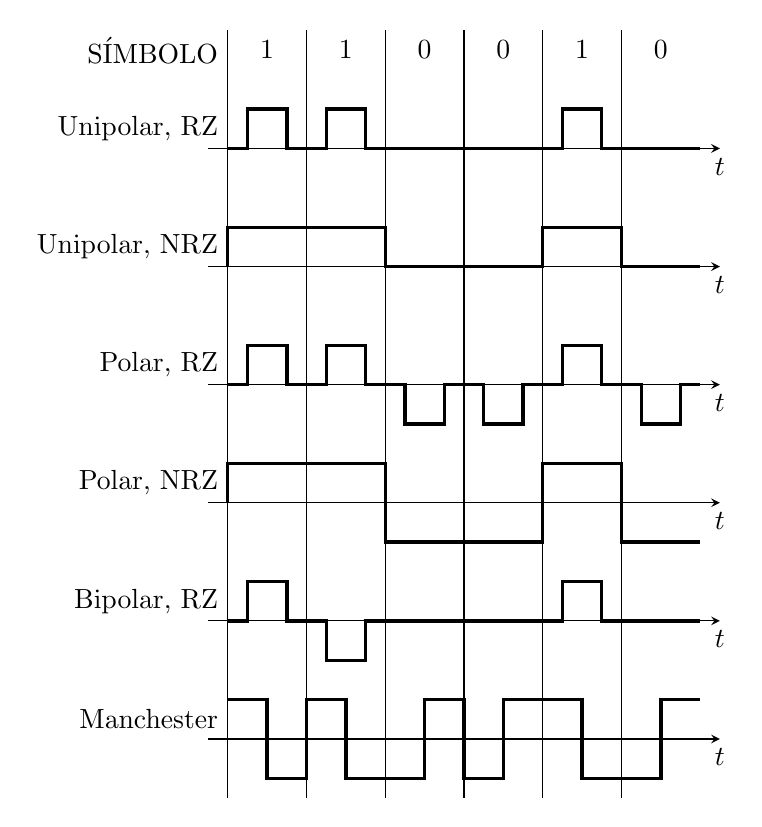
\begin{tikzpicture}[scale=0.5]
            \draw (0,1) -- (0,-18.5);
            \draw (2,1) -- (2,-18.5);
            \draw (4,1) -- (4,-18.5);
            \draw (6,1) -- (6,-18.5);
            \draw (8,1) -- (8,-18.5);
            \draw (10,1) -- (10,-18.5);
            \path (0,0.5) node [anchor=east] {SÍMBOLO} -- (1,0.5) node {$1$} -- (3,0.5) node {$1$} -- (5,0.5) node {$0$} -- (7,0.5) node {$0$} -- (9,0.5) node {$1$} -- (11,0.5) node {$0$};
            \begin{scope}[shift={(0,-2)}]
                \draw[-stealth] (-0.5,0) -- (12.5,0) node [anchor=north] {$t$};
                \path (0,0.5) node [anchor=east] {Unipolar, RZ};
                \draw[very thick] (0,0) -- (0.5,0) -- (0.5,1) -- (1.5,1) -- (1.5,0) -- (2.5,0) -- (2.5,1) -- (3.5,1) -- (3.5,0) -- (8.5,0) -- (8.5,1) -- (9.5,1) -- (9.5,0) -- (12,0);
            \end{scope}
            \begin{scope}[shift={(0,-5)}]
                \draw[-stealth] (-0.5,0) -- (12.5,0) node [anchor=north] {$t$};
                \path (0,0.5) node [anchor=east] {Unipolar, NRZ};
                \draw [very thick] (0,0) -- (0,1) -- (4,1) -- (4,0) -- (8,0) -- (8,1) -- (10,1) -- (10,0) -- (12,0);
            \end{scope}
            \begin{scope}[shift={(0,-8)}]
                \draw[-stealth] (-0.5,0) -- (12.5,0) node [anchor=north] {$t$};
                \path (0,0.5) node [anchor=east] {Polar, RZ};
                \draw [very thick] (0,0) -- (0.5,0) -- (0.5,1) -- (1.5,1) -- (1.5,0) -- (2.5,0) -- (2.5,1) -- (3.5,1) -- (3.5,0) -- (4.5,0) -- (4.5,-1) -- (5.5,-1) -- (5.5,0) -- (6.5,0) -- (6.5,-1) -- (7.5,-1) -- (7.5,0)-- (8.5,0) -- (8.5,1) -- (9.5,1) -- (9.5,0) -- (10.5,0) -- (10.5,-1) -- (11.5,-1) -- (11.5,0) -- (12,0);
            \end{scope}
            \begin{scope}[shift={(0,-11)}]
                \draw[-stealth] (-0.5,0) -- (12.5,0) node [anchor=north] {$t$};
                \path (0,0.5) node [anchor=east] {Polar, NRZ};
                \draw [very thick] (0,0) -- (0,1) -- (4,1) -- (4,-1) -- (8,-1) -- (8,1) -- (10,1) -- (10,-1) -- (12,-1);
            \end{scope}
            \begin{scope}[shift={(0,-14)}]
                \draw[-stealth] (-0.5,0) -- (12.5,0) node [anchor=north] {$t$};
                \path (0,0.5) node [anchor=east] {Bipolar, RZ};
                \draw[very thick] (0,0) -- (0.5,0) -- (0.5,1) -- (1.5,1) -- (1.5,0) -- (2.5,0) -- (2.5,-1) -- (3.5,-1) -- (3.5,0) -- (8.5,0) -- (8.5,1) -- (9.5,1) -- (9.5,0) -- (12,0);
            \end{scope}
            \begin{scope}[shift={(0,-17)}]
                \draw[-stealth] (-0.5,0) -- (12.5,0) node [anchor=north] {$t$};
                \path (0,0.5) node [anchor=east] {Manchester};
                \draw[very thick] (0,1) -- (1,1) -- (1,-1) -- (2,-1) -- (2,1) -- (3,1) -- (3,-1) -- (5,-1) -- (5,1) -- (6,1) -- (6,-1) -- (7,-1) -- (7,1) -- (9,1) -- (9,-1) -- (11,-1) -- (11,1) -- (12,1);
            \end{scope}
        \end{tikzpicture}
        \endpgfgraphicnamed\end{minipage}
    \end{figure}

\end{ejemplo}

\begin{ejemplo}[código cuaternario (polar)] 4 símbolos
    \begin{center}\begin{minipage}{\textwidth}
        \bpgf{Imagenes/codLinBB/codLinBB-2}
        \begin{tikzpicture}
            \draw (0,0) -- (0.5,0) -- (0.5,1.5) node [anchor=south east] {$3\,V$} -- (1.5,1.5) -- (1.5,0) -- (2,0);
            \draw (3,0) -- (3.5,0) -- (3.5,0.5) -- (4.5,0.5) node [anchor=south west] {$1\,V$} -- (4.5,0) -- (5,0);
            \draw (6,0) -- (6.5,0) -- (6.5,-0.5) node [anchor=north east] {$-1\,V$} -- (7.5,-0.5) -- (7.5,0) -- (8,0);
            \draw (9,0) -- (9.5,0) -- (9.5,-1.5) node [anchor=north east] {$-3\,V$} -- (10.5,-1.5) -- (10.5,0) -- (11,0);
        \end{tikzpicture}

        \endpgfgraphicnamed\end{minipage}
    \end{center}

%La codificación de línea afecta el espectro de la señal y por lo tanto su adecuación al canal.
\end{ejemplo}

La codificación de línea afecta muchas cosas:
\begin{itemize}
    \item Contenido de frecuencia de la señal, ¿tiene contínua?
    \item Extracción del reloj de sincronismo.
    \item Potencia requerida.
    \item Probabilidad de error de detección en presencia de ruido.
    \item Posibilidad de corrección de errores mediante redundancia.
\end{itemize}

\section{Densidad espectral de potencia de la señal PAM}\label{sec.densdig}

Consideramos la onda PAM (tren de pulsos modulados en amplitud)
\[
x(t) = \displaystyle\sum_k a_k p(t-kT_s).
\]
En general es difícil calcular el espectro ``de voltaje'', o sea
la transformada de Fourier de la propia señal, dado que depende de
la sucesión de símbolos que es en principio arbitraria.
Daremos sin embargo una expresión para el espectro \emph{de potencia}
de la señal PAM en función de la estadística del proceso de proceso de símbolos, y
de la forma del pulso.

Recordamos que en la Sección \ref{sec.estoc} ya se un analizó un ejemplo de este tipo: la ``onda binaria
aleatoria'' obtenida por símbolos independientes, idénticamente distribuidos (I.I.D.), $a_k=\pm 1$,
y pulsos $p(t)=p_{[0,T_s]}(t)$. Es decir, una onda PAM con codificación de línea polar,
NRZ. Interesa generalizar el estudio a otros pulsos y otras estadísticas de
símbolos.

El caso más utilizado es el siguiente: los símbolos siguen siendo I.I.D., pero con cualquier
distribución de probabilidad con media $E[a_k]=\mu$, y varianza $E[a_k^2]- \mu^2 = \sigma^2$.
El pulso $p(t)$ puede ser cualquiera de energía finita, con transformada de Fourier $\hat{P}(f)$.
 La fórmula para la densidad de potencia de la onda PAM es

\begin{center}
\col{S_x(f) = \sigma^2 f_s \left|\hat{P}(f)\right|^2 + \mu^2 f_s^2 \sum_{n=-\infty}^{+\infty}\left|\hat{P}(nf_s)\right|^2 \delta(f-nf_s)}
\end{center}

Remitimos al Apéndice \ref{appendix:pam} de estas notas para una demostración de esta fórmula, incluyendo una generalización a procesos de símbolos no necesariamente independientes. Una precisión es que para invocar la teoría de procesos estacionarios, es necesario (como en la Sección \ref{sec.estoc}) agregar a la onda un retardo aleatorio. No proseguiremos con este punto.

Analizamos lo que dice la fórmula anterior para el caso de pulsos NRZ.

\begin{ejemplo}[pulso NRZ]
    $p(t)=\begin{cases}
            1 & \text{si } 0 \leq t \leq T_s\\
            0 & \text{en otro caso}
          \end{cases}$, $\left|\hat{P}(f)\right|^2=T_s^2\sinc^2(\pi T_s f)$.

Notar que en este caso $\hat{P}(nf_s)=0$ para todo $n\neq 0$, por lo tanto el resultado es

\[S_x(f) = \sigma^2 T_s \sinc^2 (\pi T_s f) + \mu^2\delta(f).\]

    \begin{center}\begin{minipage}{\textwidth}
        \bpgf{Imagenes/codLinBB/codLinBB-3}
        \begin{tikzpicture}
            \draw [-stealth] (-6,0) -- (6,0) node [anchor=north] {$f$};
            \draw [-stealth] (0,-0.5) -- (0,4) node [anchor=east] {$S_x(f)$};
            \draw [samples=200,domain=-5:5] plot (\x,{2*(sin(3*\x r)/(3*\x))^2});
            \path (0,2) node [anchor=west] {$\sigma^2 T_s$};
            \path (-pi/3,0) node [anchor=north] {$-f_s$} -- (pi/3,0) node [anchor=north] {$f_s$} -- (2*pi/3,0) node [anchor=north] {$2 f_s$};
            \draw [very thick, -stealth] (0,0) -- (0,3.5) node [anchor=west] {$\mu^2$};
        \end{tikzpicture}
        \endpgfgraphicnamed\end{minipage}
    \end{center}

Si particularizamos al caso de la onda binaria aleatoria, $a_k=\pm 1$, I.I.D., tenemos
 $\mu=0$, $\sigma^2=1$, por lo tanto reencontramos el resultado hallado anteriormente.
 \end{ejemplo}



\subsection*{¿Qué conclusiones podemos sacar de $S_x(f)$?}

\begin{enumerate}
    \item Potencia total: $\langle x^2\rangle = \displaystyle\int_{-\infty}^{\infty} S_x(f)\d f $.
    En el ejemplo de pulsos NRZ,
    \[
     \langle x^2\rangle = \mu^2 +\sigma^2 f_s \displaystyle\int_{-\infty}^{\infty}
    \left|\hat{P}(f)\right|^2\d f = \mu^2 +\sigma^2 f_s \displaystyle\int_{-\infty}^{\infty} \left|p(t)\right|^2\d
    t = \mu^2 + \sigma^2.\]
    \item Porcentaje de potencia dentro de una banda.  Ver más abajo.
     \item Valor de continua. En el caso NRZ, si la señalización es:
    \begin{itemize}
        \item unipolar, $a_k\in \{0,A\}\Rightarrow \mu=\frac{A}{2}$, hay continua.
        \item polar, $a_k\in \{-A,A\}\Rightarrow \mu = 0$, no hay continua.
    \end{itemize}
    \item \emph{Sincronismo}: para poder sacar ``el reloj'' de la señal debería haber un $\delta$ en $f_s$ o algún múltiplo. Por lo tanto, la onda PAM con pulsos NRZ
     no provee sincronismo.
\end{enumerate}
\newpage

\begin{ejemplo}
    Veamos el caso de pulso RZ.\begin{minipage}{5cm}
                                \bpgf{Imagenes/codLinBB/codLinBB-4}
                                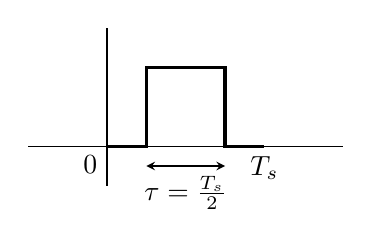
\begin{tikzpicture}[xscale=2]
                                    \draw (-0.5,0) -- (1.5,0);
                                    \draw (0,-0.5) -- (0,1.5);
                                    \path (0,0) node [anchor=north east] {$0$} -- (1,0) node [anchor=north] {$T_s$};
                                    \draw [very thick] (0,0) -- (0.25,0) -- (0.25,1) -- (0.75,1) -- (0.75,0) -- (1,0);
                                    \draw [stealth-stealth] (0.25,-0.25) -- (0.75,-0.25);
                                    \path (0.5,-0.25) node [anchor=north] {$\tau=\frac{T_s}{2}$};
                                \end{tikzpicture}
                                \endpgfgraphicnamed%\end{minipage}
                               \end{minipage}

    \[\left|\hat{P}(f)\right|^2=\left(\frac{T_s}{2}\right)^2 \sinc^2\left(\pi f \frac{T_s}{2}\right)\]

    \begin{center}\begin{minipage}{\textwidth}
        \bpgf{Imagenes/codLinBB/codLinBB-5}
        \begin{tikzpicture}
            \draw [-stealth] (-6,0) -- (6,0) node [anchor=north] {$f$};
            \draw [-stealth] (0,-0.5) -- (0,5) node [anchor=east] {$S_x(f)$};
            \draw [samples=200,domain=-5:5] plot (\x,{4*(sin(3*\x/2 r)/(3*\x/2))^2});
            \path (0,4) node [anchor=west] {$\frac{\sigma^2 T_s}{4}$};
            \path (-pi,0) node [anchor=north] {$-3 f_s$} -- (-2*pi/3,0) node [anchor=north] {$-2 f_s$} -- (-pi/3,0) node [anchor=north] {$-f_s$} -- (pi/3,0) node [anchor=north] {$f_s$} -- (2*pi/3,0) node [anchor=north] {$2 f_s$} -- (pi,0) node [anchor=north] {$3 f_s$};
            \draw [very thick, -stealth] (0,0) -- (0,2.5) node [anchor=west] {$\frac{\mu^2}{4}$};
            \draw [very thick,-stealth] (-pi,0) -- (-pi,0.25);
            \draw [very thick,-stealth] (-pi/3,0) -- (-pi/3,1);
            \draw [very thick,-stealth] (pi/3,0) -- (pi/3,1);
            \draw [very thick,-stealth] (pi,0) -- (pi,0.25);
        \end{tikzpicture}
        \endpgfgraphicnamed\end{minipage}
    \end{center}

    Aquí sí hay información de sincronismo para $\mu\neq 0$.
\end{ejemplo}

\paragraph{Pregunta} ¿Qué porcentaje de la energía de un pulso rectangular entra en las distintas bandas?

Sea $p(t)$  \begin{minipage}{5cm}
        \bpgf{Imagenes/codLinBB/codLinBB-6}
        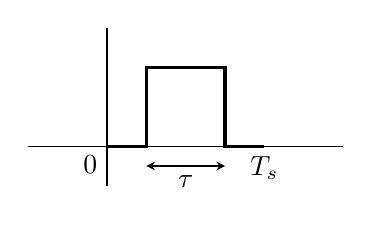
\begin{tikzpicture}[xscale=2]
            \draw (-0.5,0) -- (1.5,0);
            \draw (0,-0.5) -- (0,1.5);
            \path (0,0) node [anchor=north east] {$0$} -- (1,0) node [anchor=north] {$T_s$};
            \draw [very thick] (0,0) -- (0.25,0) -- (0.25,1) -- (0.75,1) -- (0.75,0) -- (1,0);
            \draw [stealth-stealth] (0.25,-0.25) -- (0.75,-0.25);
            \path (0.5,-0.25) node [anchor=north] {$\tau$};
        \end{tikzpicture}
        \endpgfgraphicnamed
        \end{minipage} con área $1$. $|\hat{P}(f)| = |\sinc (\pi \tau f)|$

\begin{minipage}{0.45\textwidth}
    \bpgf{Imagenes/codLinBB/codLinBB-7}
        \begin{tikzpicture}
            \draw [-stealth] (-0.5,0) -- (6,0) node [anchor=north] {$f$};
            \draw [-stealth] (0,-0.5) -- (0,5) node [anchor=west] {$\sinc^2(\pi \tau f)$};
            \draw [samples=200,domain=0.001:5] plot (\x,{4*(sin(3*\x/2 r)/(3*\x/2))^2});
            \path (0,4) node [anchor=east] {$1$};
            \draw (pi/3,0) node [anchor=north] {$\frac{1}{2\tau}$} -- (pi/3,{4*(sin(pi/2 r)/(pi/2))^2});
            \path (2*pi/3,0) node [anchor=north] {$\frac{1}{\tau}$} -- (4*pi/3,0) node [anchor=north] {$\frac{2}{\tau}$};
        \end{tikzpicture}
    \endpgfgraphicnamed
\end{minipage}
\begin{minipage}{0.2\textwidth}
    \begin{tabular}{c|c}
        $\tau f$ & \% pot\\
        \hline
        $\tfrac{1}{2}$ & $77$\\
        $1$ & $90$\\
        $2$ & $95$\\
        $3$ & $96.6$\\
        $\vdots$ & \\
        $11$ & $99$
    \end{tabular}
\end{minipage}
\begin{minipage}{0.25\textwidth}
    Se usa muchas veces $B=\tfrac{1}{\tau}$ como ancho de banda práctico.
\end{minipage}


\paragraph{Interpretación de la fórmula}

\begin{equation}
    \label{eq:dig2}S_x(f) = \sigma^2 f_s \left|\hat{P}(f)\right|^2 + \mu^2 f_s^2 \sum_{n=-\infty}^{+\infty} \left|\hat{P}(nf_s)\right|^2\delta(f-nf_s)\tag{\textasteriskcentered}
\end{equation}
Escribamos la onda PAM como superposición de dos términos:
\[x(t)= \underbrace{\sum_k (a_k-\mu) p(t-kT_s)}_{\text{aleatorio, media $0$}} +  \underbrace{\mu\sum_k p(t-kT_s)}_{\text{periódico, $z(t)$}}.\]
Analizamos por Fourier el término periódico:
\begin{align*}
    z(t) & = \mu \cdot p(t) \ast \sum_k \delta(t-kT_s)  \\
    \Rightarrow \hat{Z}(f)  & = \mu \hat{P}(f) f_s \sum_n \delta(f-nf_s) = \sum_n \mu f_s \hat{P}(nf_s) \delta(f-nf_s),
\end{align*}
de donde obtenemos la siguiente serie de Fourier:
\begin{align*}%\label{serfouz}
z(t) = \sum_n \mu f_s \hat{P}(nf_s)\e^{jn\omega_s t}.
\end{align*}
La densidad espectral de potencia de esta superposición de sinusoides es
\[S_z(f) = \sum_n \mu^2 f_s^2\left|\hat{P}(nf_s)\right|^2 \delta(f-nf_s) = \text{2º término de \eqref{eq:dig2}}.\]
Es decir que los dos términos del espectro de potencia  \eqref{eq:dig2} se interpretan como:
\begin{itemize}
    \item Un espectro continuo, que representa la parte aleatoria, con media $0$.
    \item Un espectro discreto que representa la parte determinística, periódica.
\end{itemize}


\newpage

\subsection*{Potencia de la señal digital}

Integrando la expresión \eqref{eq:dig2} en frecuencia, tenemos
\begin{align*} \langle x^2 \rangle &= \sigma^2
f_s\displaystyle\int_{-\infty}^{+\infty}\left|\hat{P}(f)\right|^2\d
f + \langle z^2\rangle \\
& = \sigma^2 \|p\|^2 f_s +\langle z^2\rangle.
\end{align*}

Aquí  $\|p\|^2 = \displaystyle\int_{-\infty}^{+\infty} p(t)^2\d t$
es la energía del pulso $p(t)$.
%
%    \begin{center}
%        \col{\langle x^2\rangle  } Potencia de señal digital.
%    \end{center}

También se acostumbra definir la \emph{energía media} del pulso aleatorio $a_k p(t-kT_s)$,
que esta dada por
\begin{align*}
    \overline{E_p} = E[a_k^2] \|p\|^2  = (\mu^2+ \sigma^2)\|p\|^2 .
\end{align*}


\noindent Hay algunos casos particulares en que la parte periódica cumple  $\langle
z^2\rangle = \mu^2 \|p\|^2 f_s$. En este caso, tendremos:
\begin{align*}
    \langle x^2\rangle  & = \overline{E_p} f_s,
\end{align*}
fórmula con interpretación intuitiva: envío un pulso de energía media $\overline{E_p}$, cada $T_s$ segundos,
la potencia media es $\overline{E_p}/T_s = \overline{E_p} f_s$. Sin embargo, para que esta interpretación sea válida es necesario que los pulsos
sucesivos sean ortogonales entre sí, lo cual se cumple sólo en algunos casos, como detallamos a continuación.


Validez de la fórmula $\langle x^2\rangle  =
{\overline{E_p}}{f_s}$:
\begin{itemize}
    \item Siempre que $\mu=0$, o sea $x(t)$ es una señal polar. Aquí la parte periódica desaparece.
    \item El pulso $p(t)$ tiene duración menor o igual a $T_s$.
    \item Los pulsos son de Nyquist ideales (definidos más adelante).
\end{itemize}

Para ver el segundo caso: si $p(t)$ tiene soporte en
$[0,T_s]\Rightarrow \mu p(t)$ es un período de $z(t)$
\[\Rightarrow \langle z^2\rangle  = \frac{1}{T_s} \int_0^{T_s} z^2(t)\d t = \frac{\mu^2}{T_s}\int_0^{T_s} p(t)^2\d t=
 \mu^2
\|p\|^2 f_s.\]
Alternativamente, notar que en este caso los pulsos $p(t-kT_s)$ y $p(t-lT_s)$ son ortogonales para $k\neq l$, ya que no se solapan. Esta ortogonalidad también se cumplirá en el tercer caso, como se verá después.

%\section{Formación de pulsos, interferencia intersimbólica}

Supongamos que se envía por un canal de ancho $B<\infty$ una onda
PAM $\sum a_k p(t-kT_s)$, con pulsos rectangulares.

\begin{figure}[htb]
    \centering\begin{minipage}{\textwidth}
    \bpgf{Imagenes/formPuls/formPuls-1}
    \begin{blockdiagram}[xscale=0.8]
        \draw (-0.5,0) -- (0,0) node [anchor=north] {$0$}-- (0,1) -- (1,1) -- (1,0) node [anchor=north] {$T_s$} -- (2,0) -- (2,-1) -- (3,-1) -- (3,0) -- (3.5,0);
        \path (2,1) node {$x(t)$};
        \begin{scope}[shift={(7,0)}]
            \matrix[column sep=10mm]{
                \node[punto] (inicio) {}; & \node[block] (pasa) {PASABAJOS}; & \node[punto] (salida) {};\\
            };
            \draw [->] (inicio) -- (pasa);
            \draw [->] (pasa) -- (salida);
        \end{scope}
        \begin{scope}[shift={(11,0)}]
            \draw (-0.5,0) -- (0.25,0);
            \draw (0.25,0) .. controls (0.4,0.15) and (0.9, 0.7) .. (1,0.5);
            \draw (1,0.5) .. controls (1.1,0.25) and (1.6, -0.5) ..(1.5,-0.5);
            \draw (1.5,-0.5) .. controls (1.6,-0.6) and (2,-1) .. (2.3,-0.5);
            \draw (2.3,-0.5) .. controls (2.5,-0.25) and (3,0) .. (3.5,0);
            \path (2,1) node {$y(t)$};
        \end{scope}
    \end{blockdiagram}
    \endpgfgraphicnamed\end{minipage}
\end{figure}
\FloatBarrier

El detector debe basarse en la señal distorsionada para determinar el símbolo transmitido en cada instante de muestreo.

\paragraph{Problemas}
\begin{itemize}
    \item Los pulsos no llegan al máximo.
    \item Interferencia Intersimbólica (ISI): los pulsos se propagan a símbolos adyacentes.
\end{itemize}

\paragraph{Cualitativamente} podemos visualizar esto mediante el {\em diagrama de ojo.}
Supongamos por ejemplo pulsos polares, RZ, rectangulares
($p_{[0,T_s]}(t)$ y $-p_{[0,T_s]}(t)$). Sincronizo un osciloscopio
con $f_s$, observo la superposición de los pulsos.

\begin{figure}[htb]
    \centering
    \bpgf{Imagenes/formPuls/formPuls-2}
    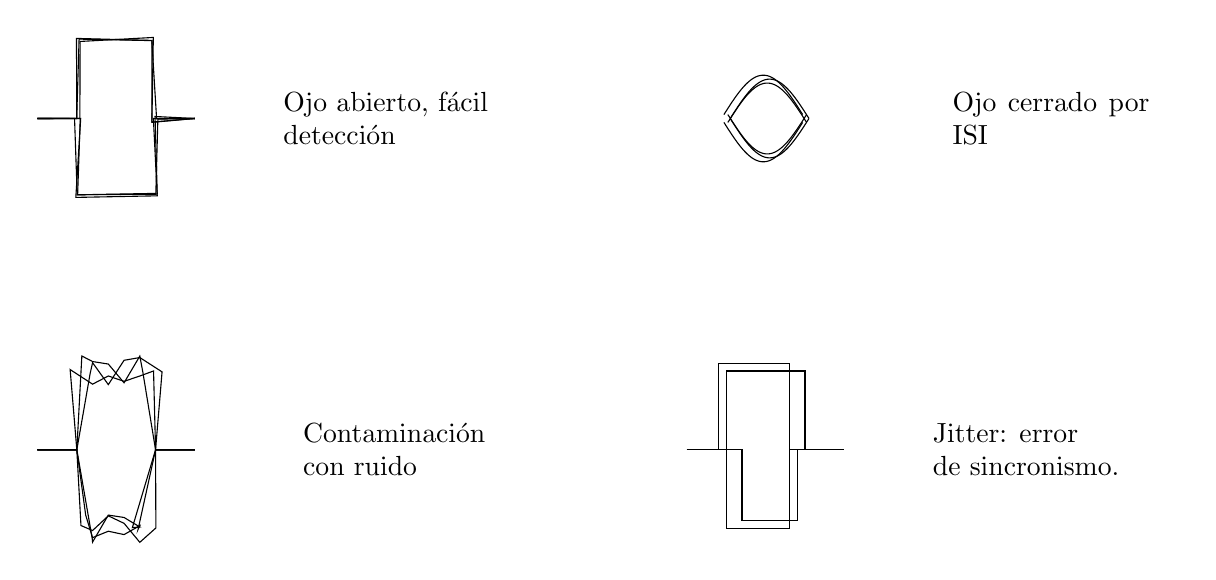
\begin{tikzpicture}
    \matrix[row sep=20mm, column sep=10mm]{
        \draw (-0.5,0) -- (0.05*rand,0.005*rand) -- (0.05*rand,1+0.05*rand) -- (1+0.05*rand,1+0.05*rand) -- (1+0.05*rand,0.05*rand) -- (1.5,0);
        \draw (-0.5,0) -- (0.05*rand,0.005*rand) -- (0.05*rand,1+0.05*rand) -- (1+0.05*rand,1+0.05*rand) -- (1+0.05*rand,0.05*rand) -- (1.5,0);
        \draw (-0.5,0) -- (0.05*rand,0.005*rand) -- (0.05*rand,1+0.05*rand) -- (1+0.05*rand,1+0.05*rand) -- (1+0.05*rand,0.05*rand) -- (1.5,0);
        \draw[yscale=-1] (-0.5,0) -- (0.05*rand,0.005*rand) -- (0.05*rand,1+0.05*rand) -- (1+0.05*rand,1+0.05*rand) -- (1+0.05*rand,0.05*rand) -- (1.5,0);
        \draw[yscale=-1] (-0.5,0) -- (0.05*rand,0.005*rand) -- (0.05*rand,1+0.05*rand) -- (1+0.05*rand,1+0.05*rand) -- (1+0.05*rand,0.05*rand) -- (1.5,0);
        \draw[yscale=-1] (-0.5,0) -- (0.05*rand,0.005*rand) -- (0.05*rand,1+0.05*rand) -- (1+0.05*rand,1+0.05*rand) -- (1+0.05*rand,0.05*rand) -- (1.5,0);
        & \path (0,0) node {\begin{minipage}{3cm}
        Ojo abierto, fácil \\detección\end{minipage}};
        & &
        \draw [domain=0:1, samples=50] plot ({\x+0.05},{0.5*sin(pi*\x r)});
        \draw [domain=0:1, samples=50] plot ({\x+0.02},{0.5*sin(pi*\x r)-0.05});
        \draw [domain=0:1, samples=50] plot ({\x-0.03},{0.5*sin(pi*\x r)+0.05});
        \draw [domain=0:1, samples=50,yscale=-1] plot ({\x+0.05},{0.5*sin(pi*\x r)});
        \draw [domain=0:1, samples=50,yscale=-1] plot ({\x+0.02},{0.5*sin(pi*\x r)-0.05});
        \draw [domain=0:1, samples=50,yscale=-1] plot ({\x-0.03},{0.5*sin(pi*\x r)+0.05});
        & \path (0,0) node {\begin{minipage}{2.5cm}
        Ojo cerrado por ISI\end{minipage}};\\

        \draw (-0.5,0) -- (0,0) -- (0+0.2*rand+0.1,1+0.2*rand) -- (0.2,1+0.2*rand) -- (0.4,1+0.2*rand) -- (0.6,1+0.2*rand) -- (0.8,1+0.2*rand) -- (1+0.2*rand-0.1,1+0.015*rand) -- (1,0) -- (1.5,0);
        \draw (-0.5,0) -- (0,0) -- (0+0.2*rand+0.1,1+0.2*rand) -- (0.2,1+0.2*rand) -- (0.4,1+0.2*rand) -- (0.6,1+0.2*rand) -- (0.8,1+0.2*rand) -- (1+0.2*rand-0.1,1+0.015*rand) -- (1,0) -- (1.5,0);
        \draw (-0.5,0) -- (0,0) -- (0+0.2*rand+0.1,1+0.2*rand) -- (0.2,1+0.2*rand) -- (0.4,1+0.2*rand) -- (0.6,1+0.2*rand) -- (0.8,1+0.2*rand) -- (1+0.2*rand-0.1,1+0.015*rand) -- (1,0) -- (1.5,0);
        \draw[yscale=-1] (-0.5,0) -- (0,0) -- (0+0.2*rand+0.1,1+0.2*rand) -- (0.2,1+0.2*rand) -- (0.4,1+0.2*rand) -- (0.6,1+0.2*rand) -- (0.8,1+0.2*rand) -- (1+0.2*rand-0.1,1+0.015*rand) -- (1,0) -- (1.5,0);
        \draw[yscale=-1] (-0.5,0) -- (0,0) -- (0+0.2*rand+0.1,1+0.2*rand) -- (0.2,1+0.2*rand) -- (0.4,1+0.2*rand) -- (0.6,1+0.2*rand) -- (0.8,1+0.2*rand) -- (1+0.2*rand-0.1,1+0.015*rand) -- (1,0) -- (1.5,0);
        \draw[yscale=-1] (-0.5,0) -- (0,0) -- (0+0.2*rand+0.1,1+0.2*rand) -- (0.2,1+0.2*rand) -- (0.4,1+0.2*rand) -- (0.6,1+0.2*rand) -- (0.8,1+0.2*rand) -- (1+0.2*rand-0.1,1+0.015*rand) -- (1,0) -- (1.5,0);
        & \path (0,0) node {\begin{minipage}{2.5cm}Contaminación con ruido\end{minipage}};
        & &
        \draw (-0.5,0) -- (0,0) -- (0,1) -- (1,1) -- (1,0) -- (1.5,0);
        \draw (-0.5,0) -- (-0.1,0) -- (-0.1,1.1) -- (0.8,1.1) -- (0.8,0) -- (1.5,0);
        \draw (-0.5,0) -- (0.2,0) -- (0.2,-0.9) -- (0.9,-0.9) -- (0.9,0) -- (1.5,0);
        \draw (-0.5,0) -- (0,0) -- (0,-1) -- (0.8,-1) -- (0.8,0) -- (1.5,0);
        & \path (0,0) node {\begin{minipage}{3cm}
        Jitter: error \\de sincronismo.\end{minipage}};\\
    };
    \end{tikzpicture}
    \endpgfgraphicnamed
\end{figure}
\FloatBarrier

\subsection*{¿Cómo analizar el problema cuantitativamente?}

Un primer enfoque sería estudiar el error $x(t)-y(t)$ en términos
de su potencia media
\[
\langle(x-y)^2\rangle = \int_{|f|>B} S_x(f)\d f.
\]
Si este error es pequeño en relación a $\langle x^2 \rangle$, es
probable que la detección funcione bien. Esto puede servir para
estimar a qué velocidad $f_s$ transmitir.

\begin{ejemplo} \mbox{}%$\phantom{1}$
\begin{center}\begin{minipage}{\textwidth}
    \bpgf{Imagenes/formPuls/formPuls-3}
    \begin{tikzpicture}
        \draw (-5,0) -- (5,0);
        \draw (0,-0.5) -- (0,5);
        \draw [samples=200,domain=-4.8:4.8] plot (\x,{4.5*(sin(2*\x r)/(2*\x))^2});
        \draw [samples=200,domain=-4.8:-pi,fill] plot (\x,{4.5*(sin(2*\x r)/(2*\x))^2});
        \draw [samples=200,domain=pi:4.8,fill] plot (\x,{4.5*(sin(2*\x r)/(2*\x))^2});
        \path (-pi,0) node [anchor=north] {$-2 f_s$} -- (-pi/2,0) node [anchor=north] {$-f_s$} -- (pi/2,0) node [anchor=north] {$f_s$} -- (pi,0) node [anchor=north] {$2 f_s$};
        \path (2,4) node {NRZ polar};
    \end{tikzpicture}
    \endpgfgraphicnamed\end{minipage}
\end{center}
Si señalilzamos a $f_s = \frac{B}{2}$, obtenemos
$\langle(x-y)^2\rangle = 5\%$ de $ \langle x^2\rangle$.
\end{ejemplo}

Sin embargo: para la detección digital, basada en muestrear la
salida en ciertos momentos, nos interesa el valor del error $x-y$
en los instantes de
   muestreo.  $\langle(x-y)^2\rangle$ me da un promedio en el tiempo que no es tan relevante. En
   particular, puedo aceptar una distorsión importante de los
   pulsos (y por tanto, un error medio grande), en la medida que no
   comprometa los instantes de detección. Estudiamos ese tema a continuación.

\subsection*{Problema de Nyquist}

Dado un canal de banda base, de ancho $B$, ¿cual es la máxima
velocidad de señalización $f_s$  a la que se puede transmitir una
onda PAM $\sum a_k p(t-kT_s)$,  permitiendo a la salida la
recuperación de los $\{a_k\}$ libre de errores? ¿Qué pulsos $p(t)$
alcanzan este máximo?

%\begin{remarksSN}
{\bf Notas:}
\begin{itemize}
        \item Aquí permitimos que los $\{a_k\}$ sean cualquier número real y deben recuperarse exactamente. En este sentido, se trata de una onda PAM analógica.
        Después particularizaremos a $\{a_k\}$ en un conjunto de símbolos $\mathcal{A}$.
        \item El problema es parecido (dual) al de muestreo, también estudiado por Nyquist. Allí buscábamos la mínima frecuencia de muestreo $f_m$ que permite reconstruir una señal $x(t)$ de banda $B$.
    \end{itemize}
%\end{remarksSN}

\paragraph{Respuesta:}
\begin{center}
    \col{f_s= 2B}
\end{center}

Para alcanzar este valor, elegimos el pulso (de Nyquist ideal)
$p(t)= \sinc (\pi f_s t)$:

\begin{center}\begin{minipage}{\textwidth}
    \bpgf{Imagenes/formPuls/formPuls-4}
    \begin{tikzpicture}
        \draw[->] (-5,0) -- (5,0) node [anchor=north] {$t$};
        \draw[->] (0,-1.5) -- (0,5) node [anchor=west] {$p(t)$};
        \path (0,4.5) node [anchor=east] {$1$};
        \draw [samples=200,domain=-4.8:4.8] plot (\x,{4.5*sin(2*\x r)/(2*\x)});
        \path (-pi,0) node [anchor=north east] {$-2 T_s$} -- (-pi/2,0) node [anchor=south east] {$-T_s$} -- (pi/2,0) node [anchor=south west] {$T_s$} -- (pi,0) node [anchor=north west] {$2 T_s$};
    \end{tikzpicture}
    \endpgfgraphicnamed

    \bpgf{Imagenes/formPuls/formPuls-5}
    \begin{tikzpicture}
        \draw[->] (-3,0) -- (3,0) node [anchor=north] {$f$};
        \draw[->] (0,-0.5) -- (0,2) node [anchor=west] {$\hat{P}(f)$};
        \draw (-2,0) node [anchor=north] {$-\frac{f_s}{2}$} -- (-2,1) -- (0,1) node [anchor=south west] {$T_s$} -- (2,1) -- (2,0) node [anchor=north] {$B=\frac{f_s}{2}$};
    \end{tikzpicture}
    \endpgfgraphicnamed\end{minipage}
\end{center}
El pulso tiene ancho de banda $B$, y por lo tanto la señal $x(t)$
pasa sin distorsión por el canal. Se recibe entonces la onda PAM
\[y(t)=x(t)=\sum_k a_k \sinc \left(\pi f_s (t-kT_s)\right).\]
Como el $\sinc$ es cero en todos los múltiplos de $T_s$ salvo
uno, se deduce que
\[y(k_0 T_s) = \sum_k a_k \sinc\left(\pi f_s (k_0-k)T_s\right) = a_{k_0}.\]
Entonces el muestreo de $y(t)$ recupera los símbolos.

Falta ver que esa velocidad de señalización no se puede superar.
Supongamos en cambio que tomo $f_s > 2B$. Consideremos el mensaje
$\{a_k\} = \ldots \quad 1 \quad 0 \quad 1 \quad 0 \quad 1\quad 0
\quad 1\quad \ldots$. \\
Para ese mensaje $x(t)$ es periódica, de período $2T_s$,
frecuencia fundamental $\frac{f_s}{2} > B$. Escribimos su serie de
Fourier  $x(t) = \sum_n \hat{X}_n\e^{jnf_s\pi t}$. En un canal
pasabajos ideal de ancho de banda $B$, se filtran todos los
armónicos salvo la continua, por tanto se recibe $y(t) \equiv
\hat{X}_0$.

 Claramente, de la continua no puedo
extraer el mensaje. En particular, la salida sería igual para el
mensaje complementario (cambiar $1$ por $0$).

\paragraph{Resumen} Dado un canal de ancho $B$, la
máxima velocidad de señalización PAM que permite la detección sin
interferencia intersimbólica es $f_s=2B$. El máximo se obtiene con
pulsos de Nyquist ideales, $p(t)=\sinc (\pi f_s t)$.

\subsubsection*{Limitaciones del pulso ideal $p(t)=\sinc (\pi f_s t)$}

Un problema obvio es que el sinc es no causal, requiere empezar en
$-\infty$. En la practica se debe truncar y retardar $p(t)$ para
poder generar algo causal. Como el sinc cae a cero en forma
relativamente lenta (como $\frac{1}{t}$) el truncado no es fácil
de hacer.

Otro problema: supongamos que hay un error de sincronización y
muestreamos en $t=\varepsilon$ en lugar de $0$:

\begin{align*}
    x(\varepsilon)  & = \sum a_k \sinc (\pi f_s \varepsilon - k\pi)\\
            & = \sum a_k \frac{\sen(\pi f_s \varepsilon) (-1)^k}{\pi f_s\varepsilon -k\pi}\\
            & = \underbrace{a_0 \frac{\sen(\pi f_s \varepsilon)}{\pi f_s \varepsilon}}_{\approx a_0} + \underbrace{\sum_{k\neq 0} a_k (-1)^k \frac{\sen(\pi f_s \varepsilon)}{\pi f_s \varepsilon - k \pi}}_{\text{término de error}}
\end{align*}

Cómo los términos decaen en valor absoluto como $\frac{1}{k}$, y
$\sum \frac{1}{k}=\infty$, se puede acumular bastante error de
ISI, donde los símbolos $a_k$ con $k\neq 0$ afectan la detección
de $a_0$.

Interesaría entonces, elegir pulsos que mantuvieran en condiciones
ideales la ISI nula, pero que caigan más rápido a $0$ con $t$, o
sea que estén más concentrados en el tiempo. Naturalmente, esto
implica más ancho de banda.

Consideremos el pulso $p(t) = \sinc (\pi f_s t) m(t)$ donde
$m(0)=1$ y $m(t)$ varía ``lento''.

\begin{figure}[htb]
    \centering\begin{minipage}{\textwidth}
    \bpgf{Imagenes/formPuls/formPuls-6}
    \begin{tikzpicture}
        \draw [samples=200,domain=-5:5] plot (\x,{3*sin(5*\x r)/(5*\x)});
        \path (2,3) node {$\sinc (\pi f_s t)$};
        \begin{scope}[shift={(0,-3)}]
            \draw [samples=201, domain=-5:5] plot (\x,{cos(5*0.1*\x r)/(1-(5/pi*0.2*\x)^2)});
            \path (2,1.5) node {$m(t)$};
        \end{scope}
    \end{tikzpicture}
    \endpgfgraphicnamed\end{minipage}
\end{figure}
\FloatBarrier

Se cumplirá $p(0)=1$, $p(kT_s) = 0 \forall\,k\neq 0$, entonces de una sucesión $\sum a_k p(t-kT_s)$ se extraen los símbolos $a_k$ por muestreo.

\paragraph{¿Qué ancho de banda tiene ese pulso? Estudiamos la convolución:} \back

\begin{figure}[htb]
    \centering\begin{minipage}{\textwidth}
    \bpgf{Imagenes/formPuls/formPuls-7}
    \begin{tikzpicture}
        \path (-2.5,1) node {$\hat{P}(f)$};
        \draw [->] (-1.5,0) -- (1.5,0);
        \draw [->] (0,-0.5) -- (0,1);
        \draw (-1,0) node [anchor=north] {$-\frac{f_s}{2}$} -- (-1,0.5) -- (1,0.5) node [anchor=south west] {$T_s$} -- (1,0) node [anchor=north] {$\frac{f_s}{2}$};
        \path (2.5,0.5) node {\Huge$\ast$};
        \begin{scope}[shift={(7,0)}]
            \path (-2.5,1) node {$\hat{M}(f)$};
            \draw [->] (-1.5,0) -- (1.5,0);
            \draw [->] (0,-0.5) -- (0,1);
            \draw [samples=200,domain=-0.5:0.5] plot (\x,{1/4*(1+cos(pi*2*\x r))});
        \end{scope}
    \end{tikzpicture}
    \endpgfgraphicnamed\end{minipage}
\end{figure}
\FloatBarrier

\noindent Elegimos $\hat{M}(f)$ de banda limitada $\dfrac{\alpha
f_s}{2}$, $0<\alpha<1$ para que espectro total no crezca mucho.

\begin{figure}[htb]
    \centering\begin{minipage}{\textwidth}
    \bpgf{Imagenes/formPuls/formPuls-8}
    \begin{tikzpicture}
        \draw [->] (-7,0) -- (7,0);
        \draw [->] (0,-6.5) -- (0,2);
        \draw (-4,0) node [anchor=north] {$-\frac{f_s}{2}$} -- (-4,1) -- (0,1) node [anchor=south west] {$T_s$} -- (4,1) -- (4,0) node [anchor=north] {$\frac{f_s}{2}$};
        \begin{scope}[shift={(0,-2)}]
            \draw [->] (-7,0) -- (7,0) node [anchor=north] {$\sigma$};
            \draw [samples=200,domain=-1:1] plot (\x,{4/pi*cos(pi*\x/2 r)});
            \path (-1,0) node [anchor=north] {$-\alpha\frac{f_s}{2}$} -- (1,0) node [anchor=north] {$\alpha\frac{f_s}{2}$};
            \path (1,1) node {$\hat{M}$};
            \path (-1,0.5) node [anchor=east] {área $1$};
        \end{scope}
            \begin{scope}[shift={(0,-4)}]
            \draw [->] (-7,0) -- (7,0);
            \begin{scope}[shift={(-5,0)}]
                \draw [samples=200,domain=-1:1] plot (\x,{4/pi*cos(pi*\x/2 r)});
                \path (1,1) node [anchor=west] {$\hat{M}(f-\sigma)$};
                \path (0,0) node [anchor=north] {$f$};
            \end{scope}
        \end{scope}
        \begin{scope}[shift={(0,-6)}]
            \draw [->] (-7,0) -- (7,0) node [anchor=north] {$\sigma$};
            \draw [samples=200,domain=-5:-3] plot (\x,{1/2*(1+cos((\x-1)*pi/2 r))}) -- (3,1);
            \draw [samples=200,domain=3:5] plot (\x,{1/2*(1-cos((\x-1)*pi/2 r))});
            \path (-5,0) node [anchor=north] {$-\frac{f_s}{2}(1+\alpha)$} -- (5,0) node [anchor=north] {$\frac{f_s}{2}(1+\alpha)$};
            \draw[very thin] (-3,1) -- (-3,0) node [anchor=north] {$-\frac{f_s}{2}(1-\alpha)$};
            \draw[very thin] (3,1) -- (3,0) node [anchor=north] {$\frac{f_s}{2}(1-\alpha)$};
            \path (0,1) node [anchor=east] {$T_s$};
            \path (5,1) node {$\hat{P}(f)$};
        \end{scope}
        \draw [dotted] (4,0) -- (4,-6);
        \draw [dotted] (-4,0) -- (-4,-6);
    \end{tikzpicture}
    \endpgfgraphicnamed\end{minipage}
\end{figure}
\FloatBarrier

\begin{remarkSN} $\hat{P}(f)$ es de banda $\frac{f_s}{2}(1+\alpha)$. El parámetro $\alpha$ se llama ``exceso de ancho de banda''.
    $\hat{P}(f)$ es constante (igual a $T_s$) en la banda $|f|\leq \frac{f_s}{2}(1-\alpha)$.  $\hat{P}(\pm \frac{f_s}{2}) = \frac{T_s}{2}$, y $\hat{P}(f)$ baja en forma simétrica alrededor de ese punto.
    %su bajada alrededor del punto
%    $(\frac{T_s}{2},)$
%
%     La bajada de  tiene simetría respecto a ese
%    punto.
\end{remarkSN}


\begin{ejemplo}[Pulso de coseno alzado]
\begin{align*}
\hat{P}(f) & =
\begin{cases}
 T_s, & |f| \leq (1-\alpha) \frac{f_s}{2}  \\
 T_s \Big[\frac{1}{2} + \frac{1}{2} \cos\Big(\pi
\frac{|f|-(1-\alpha) \frac{f_s}{2} } {\alpha f_s} \Big)\Big], &
(1-\alpha) \frac{f_s}{2}  < |f| <
(1+\alpha) \frac{f_s}{2}  \\
0,&  |f| \geq (1+\alpha) \frac{ f_s}{2}
\end{cases}%\\
%p(t) & = \frac{\cos(\pi\alpha f_st)}{1-(2\alpha f_s t)^2} \
%\sinc(\pi f_s t)
\end{align*}
%  \[\frac{T_s}{2}\left\lbrace 1 \pm \cos\left[\left(f-\frac{f_s}{2}(1-\alpha)\right)\right]\right\rbrace\]
    Esto corresponde a $\hat{M}(f)=\frac{\alpha f_s}{2 \pi}\cos\left(\frac{\pi f}{\alpha
f_s}\right)\qquad \text{ con }f \in
\left[-\alpha\frac{f_s}{2},\alpha\frac{f_s}{2}\right]$.

    Ecuación en el tiempo:
    \begin{align*}
        m(t)    = \mathcal{F}^{-1}\left[\hat{M}(f)\right] = \frac{\cos(\pi \alpha f_s t)}{1-(2 f_s \alpha t)^2}
    \end{align*}
\[ \Rightarrow \col{p(t) = \frac{\cos(\pi \alpha f_s t)}{1-(2 f_s \alpha t)^2} \sinc (\pi f_s
t)}\] En particular $p(t)$ cae como $\frac{1}{t^3}$, mucho más
concentrado en el tiempo.
    \FloatBarrier
    \begin{figure}[htb]
        \centering\begin{minipage}{\textwidth}
        \bpgf{Imagenes/formPuls/formPuls-9}
        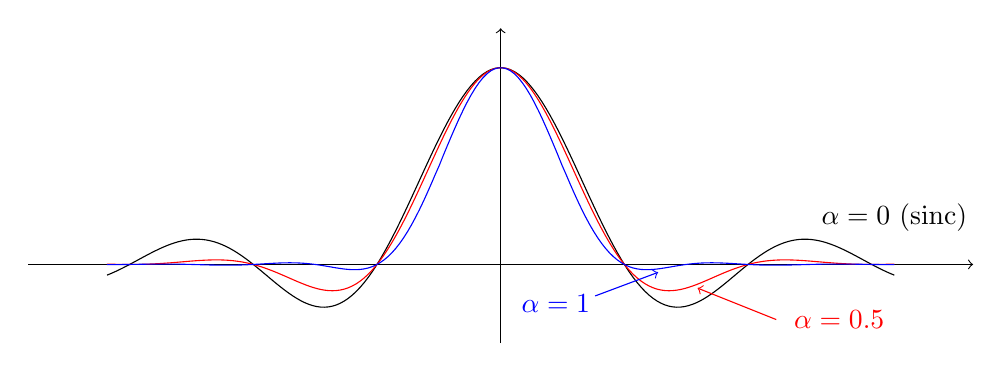
\begin{tikzpicture}
            \draw [->] (0,-1) -- (0,3);
            \draw [->] (-6,0) -- (6,0);
            \draw [samples=200,domain=-5:5] plot (\x, {2.5*sin(2*\x r)/(2*\x)});
            \draw [samples=200,domain=-5:5,red] plot (\x, {2.5*sin(2*\x r)/(2*\x)*cos(\x r)/(1-(2/pi*\x)^2)});
            \draw [samples=200,domain=-5:5,blue] plot (\x, {2.5*sin(2*\x r)/(2*\x)*cos(2*\x r)/(1-(4/pi*\x)^2)});
            \path (5,0.6) node {$\alpha=0$ (sinc)};
            \path (4.3,-.7) [red] node {$\alpha=0.5 $};
            \path [blue] (0.7,-0.5) node {$\alpha=1 $};
            \draw [->] [red] (3.5,-.7) -- (2.5,-0.3);
            \draw [->] [blue] (1.2,-0.4) -- (2,-0.1);
        \end{tikzpicture}
        \endpgfgraphicnamed\end{minipage}
    \end{figure}


\end{ejemplo}
\FloatBarrier

\subsection*{Otra forma de caracterizar los pulsos de Nyquist}

Imponemos que $p(t)$ cumpla $\begin{cases}
                                p(kT_s) = 0,& k\neq 0\\
                                p(0) = 1
                             \end{cases}$, $\hat{P}(f)$ de banda a lo sumo $2\cdot \frac{f_S}{2} = f_s$.

Estas dos condiciones se escriben como:
\begin{align*}
    p(t) \sum_{k=-\infty}^{+\infty} \delta(t-kT_s) &= \delta(t) \\
    \Leftrightarrow\hat{P}(f)\ast \frac{1}{T_s} \sum_{n=-\infty}^{+\infty} \delta(f-n f_s) &\equiv  1 \\
  \Leftrightarrow  \sum_{n=-\infty}^{+\infty} \hat{P}(f-n f_s) &\equiv
  T_s.
\end{align*}

\begin{minipage}{0.5\textwidth}
    \resizebox{\textwidth}{!}{
    \bpgf{Imagenes/formPuls/formPuls-10}
    \begin{tikzpicture}
        \draw [->] (-5,0) -- (5,0) node [anchor=north] {$f$};
        \draw [->] (0,-0.5) -- (0,1.5) node [anchor=west] {$\hat{P}$};
        \draw (2,0) .. controls (1,0) and (1,1) .. (0,1);
        \draw (-2,0) .. controls (-1,0) and (-1,1) .. (0,1);
        \draw [dotted] (0,0) .. controls (1,0) and (1,1) .. (2,1) .. controls (3,1) and (3,0) .. (4,0);
        \draw [dotted] (0,0) .. controls (-1,0) and (-1,1) .. (-2,1) .. controls (-3,1) and (-3,0) .. (-4,0);
        \path (-2,0) node [anchor=north] {$-f_s$};
        \draw [dashed] (1,1.2) -- (1,0) node [anchor=north] {$\frac{f_s}{2}$};
        \draw [dashed] (2,1.2) -- (2,0) node [anchor=north] {$f_s$};
    \end{tikzpicture}
    \endpgfgraphicnamed
    }
\end{minipage}
Sólo $2$ copias se superponen en $[0,f_s)$.

\begin{minipage}{0.3\textwidth}
    Que la suma sea constante $\Rightarrow$ simetría respecto a $\frac{f_s}{2}$
\end{minipage}
\begin{minipage}{0.5\textwidth}
    \resizebox{\textwidth}{!}{
    \bpgf{Imagenes/formPuls/formPuls-11}
    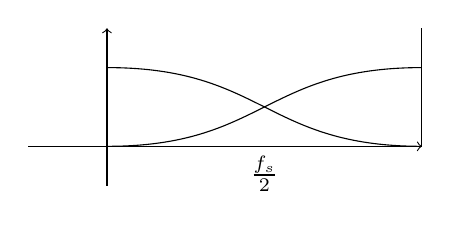
\begin{tikzpicture}[xscale=2]
        \draw [->] (-0.5,0) -- (2,0);
        \draw [->] (0,-0.5) -- (0,1.5);
        \draw (2,0) -- (2,1.5);
        \draw (2,0) .. controls (1,0) and (1,1) .. (0,1);
        \draw (0,0) .. controls (1,0) and (1,1) .. (2,1);
        \path (1,0) node [anchor=north] {$\frac{f_s}{2}$};
    \end{tikzpicture}
    \endpgfgraphicnamed
    }
\end{minipage}

\subsection*{Volvemos al tema de la eficiencia espectral}

\paragraph{Recordar}
    \begin{itemize}
        \item $f_s$: velocidad de señalización en Baudios
        ($\rfrac{\text{símb}}{\text{seg}}$).
        \item $vti = f_s \log_2 (M)$: velocidad de transmisión de información, bps.
        \item Eficiencia espectral: $\dfrac{vti}{B}$.
    \end{itemize}

   \noindent De acuerdo a Nyquist, la máxima eficiencia espectral que permite detección libre de ISI es
    \[\max_{f_s\leq 2B} \frac{f_s \log_2(M)}{B} = 2 \log_2 (M).\]

    \noindent Si en cambio, uso pulsos de Nyquist con exceso de ancho de banda $\alpha$, tenemos
    \[\frac{f_s}{2}(1+\alpha) = B \Rightarrow \text{ eficiencia espectral } \ \ \frac{2}{1+\alpha} \log_2 (M).\]

{\bf Nota:} Con $M$ arbitrario, en principio no hay límites a la
eficiencia espectral alcanzable. Sin embargo, para distinguir
símbolos en presencia de ruido, hay que separarlos (como se verá).
Agrandar $M$ implica entonces agrandar la amplitud de la señal y
por tanto la \emph{potencia}. Agrandar $vti$ para $B$ fijo tiene
un costo en potencia.
%
%
%        \begin{itemize}
%            \item Con
%            \item Sin
%        \end{itemize}
%%    \end{remarkSN}

\subsection*{Ecualización}

En diversas situaciones la interferencia intersimbólica no se
logra evitar, y se recibe una onda $x_R(t) = \sum a_k
\tilde{p}(t-kT_s)$ donde el pulso $\tilde{p}(t)$ tiene ISI.

\begin{figure}[htb]
    \centering\begin{minipage}{\textwidth}
    \bpgf{Imagenes/formPuls/formPuls-12}
    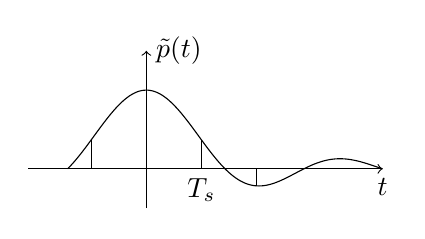
\begin{tikzpicture}
        \draw[->] (-1.5,0) -- (3,0) node [anchor=north] {$t$};
        \draw [->] (0,-0.5) -- (0,1.5) node [anchor=west] {$\tilde{p}(t)$};
        \draw [domain=-1:3,samples=200] plot (\x,{sin(pi*\x r)/(pi*\x)});
        \draw (0.7,{sin(pi*0.7 r)/(pi*0.7)}) -- (0.7,0) node [anchor=north] {$T_s$};
        \draw (-0.7,{sin(pi*(-0.7) r)/(-pi*0.7)}) -- (-0.7,0);
        \draw (1.4,{sin(pi*1.4 r)/(pi*1.4)}) -- (1.4,0);
    \end{tikzpicture}
    \endpgfgraphicnamed\end{minipage}
\end{figure}

Por ejemplo, se enviaron pulsos rectangulares por un canal muy
angosto. Una posible solución  en el receptor es compensar con un
\emph{filtro ecualizador} $\hat{H}_e$, que esencialmente invierte
el canal en la banda de interés. Una forma popular de hacerlo es
por un filtro transversal:

\begin{figure}[htb]
    \centering
    \resizebox{\textwidth}{!}{
    \bpgf{Imagenes/formPuls/formPuls-13}
    \begin{blockdiagram}
        \matrix[row sep=5 mm, column sep=10mm]{
            \node [etiqueta] (inicio) {$x_R(t)$}; & \node [punto] (p1) {}; & \node [block] (T1) {$T_s$}; & \node [punto] (p2) {}; & \node [block] (T2) {$T_s$}; & \node[punto] (p3) {}; & & \node [etiqueta]  {$\cdots$}; &  & \node [punto] (p4) {}; & \node [block] (T3) {$T_s$};\\
            & \node [multD] (m1) {$c_{-N}$}; & & \node[multD] (m2) {$c_{-N+1}$}; & & & &  & & & & \node [multD] (m3) {$c_{N}$};\\
            & & & \node [operator] (sum1) {$+$}; & & \node [operator] (sum2) {$+$}; & \node [punto] (p5) {};& &\node [etiqueta]  {$\cdots$}; & & \node [punto] (p6) {};&\node [operator] (sum3) {$+$}; & \node [etiqueta] (salida) {$y(t)$};\\
        };
        \draw (inicio) -- (p1);
        \draw [-stealth] (p1) -- (T1);
        \draw (T1) -- (p2);
        \draw [-stealth] (p2) -- (T2);
        \draw [-stealth] (T2) -- (p3);
        \draw [-stealth] (p4) -- (T3);
        \draw [-stealth] (p1) -- (m1);
        \draw [-stealth] (p2) -- (m2);
        \draw [-stealth] (T3) -|  (m3);
        \draw [-stealth] (m1) |- (sum1);
        \draw [-stealth] (m2) -- (sum1);
        \draw [-stealth] (sum1) -- (sum2);
        \draw [-stealth] (sum2) -- (p5);
        \draw [-stealth] (p6) -- (sum3);
        \draw [-stealth] (m3) -- (sum3);
        \draw [-stealth] (sum3) -- (salida);
    \end{blockdiagram}
    \endpgfgraphicnamed
}
\end{figure}
%\[
%\hat{H}(f) = \left (\sum_{k=-N}^N c_k \e^{-j2\pi f k
%%T_s}\right)\e^{-j2\pi f k N T_s}
%\]
\begin{align*} y(t+NT_s) = \sum_{n=-N}^N c_n {x}_R(t-nT_s) =\sum_{n=-N}^N
c_n \sum_k a_k \tilde{p}(t-(k+n)T_s) =\sum_k a_k\hat{p}(t - kT_s),%
%\\
%\text{donde }\hat{p}(t) =\sum_{n=-N}^N c_n \tilde{p}(t-nT_s)
%\Longrightarrow \mbox{ salida es una onda PAM con pulso
%$\hat{p}(t)$, retardada $NT_s$.}
\end{align*}%
donde $\hat{p}(t) =\sum_{n=-N}^N c_n \tilde{p}(t-nT_s)
\Longrightarrow y(t)$ es una onda PAM con pulso $\hat{p}(t)$,
retardada $NT_s$.

La idea es elegir los $\{c_n\}$ de modo de {\em forzar los ceros}
$\hat{p}(kT_s) = 0$ para $k\pm 1, \pm 2,\ldots,\pm N$. Esto se
denomina Zero Forcing Equalizer (ZFE), y  asegura que no hay ISI
con los $N$ símbolos adyacentes.  Estas condiciones,
conjuntamente con $\hat{p}(0)=1$, dan
 $2N+1$ ecuaciones para determinar las $2N+1$ ganancias $c_n$.
Como dato para ajustar el filtro debemos conocer
$\tilde{p}(kT_s)$, lo cual puede obtenerse de un experimento.
También hay versiones con ajuste adaptativo.

%\section{Detección digital en presencia de ruido}

\begin{figure}[htb]
    \centering\begin{minipage}{\textwidth}
    \bpgf{Imagenes/detDig/detDig-1}
    \begin{blockdiagram}
        \matrix[row sep=5 mm, column sep=10mm]{
            & & & \node[punto] (p1) {}; & \node[etiqueta] (muestreo) {} node [anchor=south]{muestreo} ;\\
            \node [punto] (inicio) {} node [anchor=east] {$\sum_k a_k p(t-kT_s) + n(t)$}; & \node [punto] (p2) {}; &\node [punto] (p3) {}; & &\node [punto] (p4) {} node [anchor=north] {$y$}; &\node [block] (comp) {COMP}; &\node [etiqueta] (salida) {$\hat{a}_k$}; \\
            & & \node [block] (sinc) {SINCR}; & \node [punto] (p5) {};\\
        };
        \draw (inicio) -- (p2) -- (p3) -- (muestreo);
        \draw [->] (p2) |- (sinc);
        \draw (sinc) -- (p5);
        \draw [->,dashed] (p5) -- (p1);
        \draw [->] (p4) -- (comp);
        \draw [->] (comp) -- (salida);
    \end{blockdiagram}
    \endpgfgraphicnamed\end{minipage}
\end{figure}
\FloatBarrier

Recibo la onda digital de banda base contaminada de ruido. Suponemos por ahora:
\begin{itemize}
    \item Sincronización perfecta.
    \item No hay ISI. O sea que los pulsos son de Nyquist o que tengo ancho de banda suficiente para que pasen pulsos rectangulares sin distorsión apreciable.
    \item A la entrada del comparador, tenemos la muestra $y_k = a_k + n_k$, donde \\
%\begin{itemize}
%\item $a_k$ es el símbolo transmitido.%una muestra de ruido
%\item $n_k$ es una muestra de ruido
%\end{itemize}
$\begin{cases}
a_k \in \mathcal{A} & \text{ es el símbolo transmitido}\\
n_k=n(kT_s) & \text{ es una muestra de ruido}
\end{cases}$.
\end{itemize}

Suponemos que $n_k$ tiene $E[n_k]=0$, $E[n_k^2]=\sigma^2$, y
densidad de probabilidad $f_N(n)$.

\begin{minipage}{0.5\textwidth}
    \bpgf{Imagenes/detDig/detDig-2}
    \begin{tikzpicture}
        \draw [->] (-3,0) -- (3,0) node [anchor=north] {$n$};
        \draw [->] (0,-0.5) -- (0,2.5) node [anchor=west] {$f_N(n)$};
        \draw [domain=-2.5:2.5,samples=200] plot (\x,{2*exp(-1*((\x)^2))});
    \end{tikzpicture}
    \endpgfgraphicnamed
\end{minipage}
\begin{minipage}{0.5\textwidth}
\[\int_a^b f_N(n)\d n = Prob (a\leq n_k \leq b).\]
\end{minipage}

Por ahora no entramos en el tema de cómo el ruido $n(t)$ se generó
en el canal analógico. Típicamente, será un ruido blanco que se
filtra en recepción. Postergamos ese análisis.

\subsection*{Probabilidad de error de detección, s\'imbolos binarios}

Consideramos primero el caso binario, donde $a_k$ toma dos valores
posibles, $A_1 < A_2$. \\ Por ejemplo: $A_1=0, A_2 = A$ en el caso
unipolar.

La densidad de probabilidad de la V.A. $Y$ recibida, es la de $n$
trasladada por el símbolo. Tenemos por tanto $2$ densidades
\emph{condicionales} al símbolo enviado,
\begin{gather*}
    f_{Y|A_1} (y) = f_N(y-A_1);\\
    f_{Y|A_2} (y) = f_N(y-A_2).
\end{gather*}

\begin{figure}[htb]
    \centering\begin{minipage}{\textwidth}
    \bpgf{Imagenes/detDig/detDig-3}
    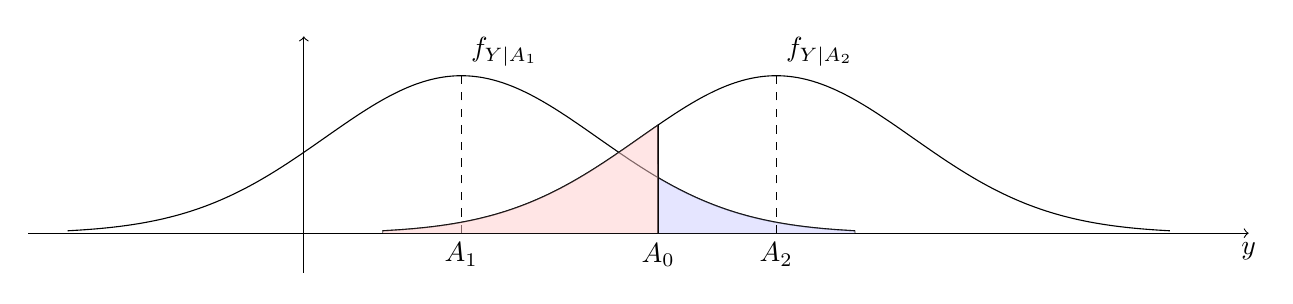
\begin{tikzpicture}
        \draw [->] (-3.5,0) -- (12,0) node [anchor=north] {$y$};
        \draw [->] (0,-0.5) -- (0,2.5);
        \draw [domain=-3:7,samples=200] plot (\x,{2*exp(-1*((\x-2)^2)/6)});
        \draw [dashed] (2,0) node [anchor=north] {$A_1$} -- (2,2) node [anchor=south west] {$f_{Y|A_1}$};
        \draw [domain=4.5:7,samples=200,fill=blue!20,opacity=0.5] (4.5,0) --  plot (\x,{2*exp(-1*((\x-2)^2)/6)}) -- (7,0);
        \begin{scope}[shift={(4,0)}]
            \draw [domain=-3:7,samples=200] plot (\x,{2*exp(-1*((\x-2)^2)/6)});
            \draw [dashed] (2,0) node [anchor=north] {$A_2$} -- (2,2) node [anchor=south west] {$f_{Y|A_2}$};
            \draw [thick] (0.5,0) node [anchor=north] {$A_0$} -- (0.5,{2*exp(-1*(1.5^2)/6)});
            \draw [domain=-3:0.5,samples=200,fill=red!20,opacity=0.5] (-3,0) --  plot (\x,{2*exp(-1*((\x-2)^2)/6)}) -- (0.5,0);
        \end{scope}
    \end{tikzpicture}
    \endpgfgraphicnamed\end{minipage}
\end{figure}
\FloatBarrier

Decidimos si se transmitió $A_1$ o $A_2$ comparando con un umbral
$A_0$. Entonces hay un error de detección si:
\begin{itemize}
    \item $y>A_0$ y se transmitió $A_1$;
    \item $y<A_0$ y  se transmitió $A_2$.
\end{itemize}

Calculo la probabilidad de cada evento, indicada en sombreado.
\begin{align*}
    P(\text{error}|A_1) &= \int_{A_0}^\infty f_N(y-A_1)\d y = \int_{A_0-A_1}^\infty f_N(n)\d n;\\
    P(\text{error}|A_2) &= \int_{-\infty}^{A_0} f_N(y-A_2)\d y = \int_{-\infty}^{-(A_2-A_0)} f_N(n)\d n.\\
\end{align*}

\begin{figure}[htb]
    \centering\begin{minipage}{\textwidth}
    \bpgf{Imagenes/detDig/detDig-4}
    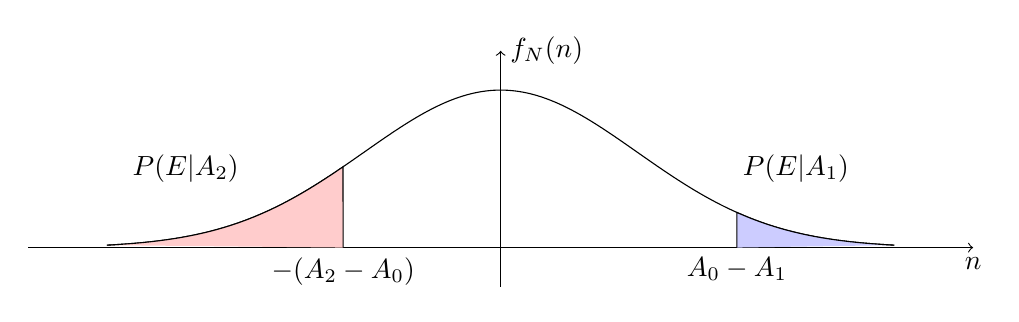
\begin{tikzpicture}
        \draw [->] (-6,0) -- (6,0) node [anchor=north] {$n$};
        \draw [->] (0,-0.5) -- (0,2.5) node [anchor=west] {$f_N(n)$};
        \draw [domain=-5:5,samples=200] plot (\x,{2*exp(-1*((\x)^2)/6)});
        \draw [domain=-5:-2,samples=200,fill=red!20] plot (\x,{2*exp(-1*((\x)^2)/6)}) -- (-2,0) node [anchor=north] {$-(A_2-A_0)$};
        \draw [domain=3:5,samples=200,fill=blue!20] (3,0) node [anchor=north] {$A_0-A_1$} -- plot (\x,{2*exp(-1*((\x)^2)/6)});
        \path (-4,1) node {$P(E|A_2)$};
        \path (3.75,1) node {$P(E|A_1)$};
    \end{tikzpicture}
    \endpgfgraphicnamed\end{minipage}
\end{figure}
\FloatBarrier

Esas son probabilidades condicionales. La probabilidad total es:
\[P_e = P(E|A_1) P (A_1) + P(E|A_2) P (A_2).\]

\subsubsection*{Umbral óptimo}

Si subimos el umbral $A_0$, $P(E|A_1)$ baja pero sube $P(E|A_2)$,
y viceversa. Entonces hay un compromiso en la elección del umbral.
La selección óptima es la que minimiza $P_e$; la hallamos por
diferenciación.

\[\frac{\partial P_e}{\partial A_0} = P(A_2) f_N(A_0 - A_2) - P(A_1) f_N (A_0 - A_1).\]

Existe $A_0^*$ que anula la derivada, que cumple
\[\frac{P(A_2)}{P(A_1)}=\frac{f_N(A_0^*-A_1)}{f_N(A_0^*-A_2)}.\]

\subsubsection*{Caso usual: símbolos equiprobables, ruido simétrico}

$P(A_1) = P(A_2) = \frac{1}{2}\Rightarrow f_N(A_0^*-A_1) =
f_N(A_0^*-A_2)$.

Supongamos $f_N(n)$ simétrica (par) y decreciente en $n>0$ (caso típico: Gaussiana).

\begin{figure}[htb]
    \centering\begin{minipage}{\textwidth}
    \bpgf{Imagenes/detDig/detDig-5}
    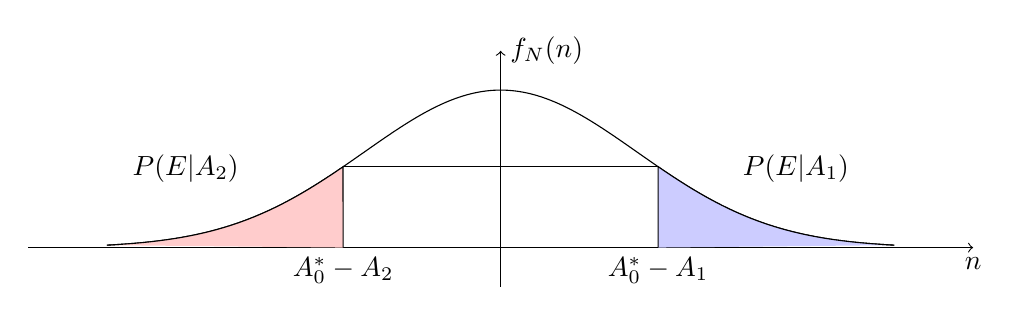
\begin{tikzpicture}
        \draw [->] (-6,0) -- (6,0) node [anchor=north] {$n$};
        \draw [->] (0,-0.5) -- (0,2.5) node [anchor=west] {$f_N(n)$};
        \draw [domain=-5:5,samples=200] plot (\x,{2*exp(-1*((\x)^2)/6)});
        \draw [domain=-5:-2,samples=200,fill=red!20] plot (\x,{2*exp(-1*((\x)^2)/6)}) -- (-2,0) node [anchor=north] {$A_0^*-A_2$};
        \draw [domain=2:5,samples=200,fill=blue!20] (2,0) node [anchor=north] {$A_0^*-A_1$} -- plot (\x,{2*exp(-1*((\x)^2)/6)});
        \path (-4,1) node {$P(E|A_2)$};
        \path (3.75,1) node {$P(E|A_1)$};
        \draw (2,{2*exp(-2/3)}) -- (-2,{2*exp(-2/3)});
    \end{tikzpicture}
    \endpgfgraphicnamed\end{minipage}
\end{figure}

Para que sean iguales las $f_N$, $A_2-A_0^* = A_0^*-A_1
\Rightarrow A_0^*=\dfrac{A_1+A_2}{2}$. \\
También $P(E|A_1) =
P(E|A_2)$. En este caso:
\[
{\col{P_e= P(E|A_1) = P(E|A_2) = \int_{\frac{A_2-A_1}{2}}^\infty
f_N(n)\d n}}
\]
Si en cambio, $P(A_2) > P(A_1)$ por ejemplo, entonces
$f_N(A_0^*-A_1) > f_N(A_0^*-A_2) \Rightarrow A_0^*-A_1 <
A_2-A_0^*$. El umbral óptimo está más cerca del símbolo menos
probable.

\subsection*{Probabilidad de error óptima, binario, ruido Gaussiano}
El modelo más usado para la distribución de probabilidad del ruido
es la normal o Gaussiana:
\[f_N(n) = \frac{1}{\sqrt{2\pi}\sigma}\e^{-\frac{n^2}{2\sigma^2}}\qquad \text{ (media $0$, varianza $\sigma^2$)}.\]
Denotamos por $Q(z)$ la probabilidad de que una normal standard
($\sigma=1$) supere a $z$,
\[Q(z):=\frac{1}{\sqrt{2\pi}} \int_z^\infty \e^{-\frac{n^2}{2}}\d n.\]
\begin{itemize}
    \item No tiene expresión analítica, pero está tabulada.
    \item Para $z \gg 1$, vale la aproximación $Q(z)\approx
    \frac{1}{\sqrt{2\pi}z}\e^{-\frac{z^2}{2}}$.
\end{itemize}

Si tengo un ruido $n$ normal $(0,\sigma^2)$, entonces $\frac{n}{\sigma}$ tiene varianza $1$. Por tanto,
\[P(n>z) = P \left(\frac{n}{\sigma}>\frac{z}{\sigma}\right) = Q\left(\frac{z}{\sigma}\right).\]

Entonces, para la detección con símbolos binarios equiprobables,
ruido Gaussiano $(0,\sigma^2)$, llegamos a la siguiente fórmula
para la probabilidad de error:
\[P_e=\int_{\frac{A_2-A_1}{2}}^\infty f_N(n)\d n = P\left(n>\frac{A_2-A_1}{2}\right) = Q\left(\frac{A_2-A_1}{2\sigma}\right).\]

\begin{ejemplo}[binario, equiprobable, ruido Gaussiano]$\phantom{1}$
\begin{description}
    \item[Unipolar] $A_1=0$, $A_2=A$, $A_0^* = \frac{A}{2}$,
    $P_e=Q\left(\frac{A}{2\sigma}\right)$.
    \item[Polar] $A_1=-A$, $A_2=A$, $A_0^* = 0$, $P_e =
    Q\left(\frac{A}{\sigma}\right)$.
 \end{description}
Notar que en ambos casos, para reducir $P_e$, debo aumentar
$\frac{A}{\sigma}$. De hecho, $P_e$ cae muy rápidamente:
%\begin{remarkSN}$\phantom{1}$
%    \begin{itemize}
%        \item Para achicar  \\
        \begin{center}
            \begin{tabular}{c|c}
                $\frac{A}{\sigma}$ & $Q\left(\frac{A}{\sigma}\right)=P_e(\text{polar})$\\
                \hline
                $2$ & $0.022$\\
                $4$ & $3\cdot 10^{-5}$\\
                $6$ & $10^{-8}$
            \end{tabular}
        \end{center}
\end{ejemplo}
%
%        Cae muy
%        \item
%    \end{itemize}
%\end{remarkSN}
$\frac{A}{\sigma}$ opera como una relación señal - ruido. De
hecho, $\sigma^2=E[n_k^2]=N$, potencia media de ruido. $A^2$ está
relacionado con la potencia de la onda $x(t) = \sum a_k
p(t-kT_s)$. La relación exacta depende de $p(t)$ y el código de
línea, veamos ejemplos.


\begin{ejemplo}
    $p(t)= p_{[0,T_s]}(t)$ NRZ. En este caso, vimos que $\langle x^2 \rangle = E[a_k^2]\frac{\|p\|^2}{T_s} =
    E[a_k^2]$. Casos particulares:
    \begin{align*}
    \text{Polar, NRZ: } \langle x^2 \rangle  &= A^2 \Rightarrow \left(\frac{S}{N}\right) = \frac{A^2}{\sigma^2}.\\
    \text{Unipolar,NRZ: } \langle x^2 \rangle &=\frac{A^2}{2}\Rightarrow \left(\frac{S}{N}\right) =
    \frac{A^2}{2\sigma^2}.
\end{align*}
    \begin{equation*}
        \Rightarrow \left.\begin{aligned}
                        P_e = Q\left(\sqrt{\frac{S}{N}}\right)\qquad &\text{polar}\\
                        P_e = Q\left(\frac{1}{\sqrt{2}}\sqrt{\frac{S}{N}}\right)\qquad &\text{unipolar}
                    \end{aligned} \right\rbrace
                    \text{\begin{minipage}{5cm}
                            polar es más eficiente: menor $P_e$ para igual
                            $\frac{S}{N}$.
                          \end{minipage}}
    \end{equation*}
\end{ejemplo}

\subsection*{Caso M-ario ($M$ símbolos por pulso)}

Elegimos una ``constelación'' de niveles para representar los $M$ símbolos. Por ejemplo, para $M$ par, elegimos una constelación polar $\{\pm A, \pm 3A,\pm 5A,\ldots\}$. El espaciamiento es $2A$. El nivel más grande es $(M-1)A$. Tomamos símbolos equiprobables y contaminamos con ruido Gaussiano, tenemos:

\begin{figure}[htb]
    \centering\begin{minipage}{\textwidth}
    \bpgf{Imagenes/detDig/detDig-6}
    {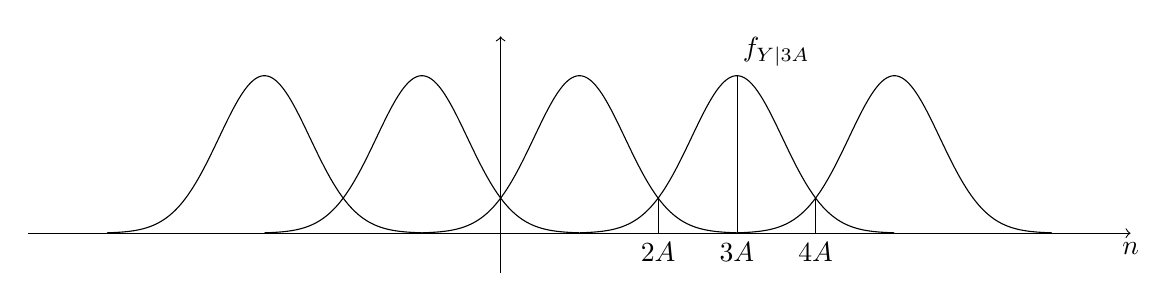
\begin{tikzpicture}
        \draw [->] (-6,0) -- (8,0) node [anchor=north] {$n$};
        \draw [->] (0,-0.5) -- (0,2.5);
        \foreach \a in {-3,-1,1,3,5}
            \draw [domain={\a-2}:{\a+2},samples=200] plot (\x,{2*exp(-1.5*((\x-\a)^2))});
        \path (3.5,2) node [anchor=south] {$f_{Y|3A}$};
        \draw [ultra thin] (2,0) node [anchor=north] {$2A$} -- (2,{2*exp(-1.5)});
        \draw [ultra thin] (4,0) node [anchor=north] {$4A$} -- (4,{2*exp(-1.5)});
        \draw [ultra thin] (3,0) node [anchor=north] {$3A$} -- (3,2);
    \end{tikzpicture}}
    \endpgfgraphicnamed\end{minipage}
\end{figure}
\FloatBarrier

Es intuitivo que los umbrales de detección óptimos son los puntos medios $0,\pm 2A, \pm 4A,\ldots$

Para cualquier símbolo menos los extremos
\[P(E|\text{simb}) = P(|n|>A) = 2P(n>A) = 2Q\left(\frac{A}{\sigma}\right).\]
Para los extremos
\[P(E|\text{simb}) = Q\left(\frac{A}{\sigma}\right).\]

\paragraph{TOTAL}

\[P_e=\frac{(M-2) 2 Q\left(\frac{A}{\sigma}\right) + 2Q\left(\frac{A}{\sigma}\right)}{M} = \underbrace{2\left(\frac{M-1}{M}\right)Q\left(\frac{A}{\sigma}\right)}_{\text{prob. error de símbolo}}.\]

Si queremos relacionar $P_e$ con $\left(\frac{S}{N}\right)$, otra
vez jugaría la forma de los pulsos.

\begin{ejemplo}
    Pulsos NRZ, $a_k$ polar M-ario.
    \[\langle x^2\rangle=E[a_k^2]=A^2\frac{2}{M}\left(1+3^2+5^2+\cdots+(M-1)^2\right) = \frac{2A^2}{M}\left(\frac{M^3-M}{6}\right) = \frac{A^2(M^2-1)}{3}\]

  Se utilizó arriba una fórmula para la suma de los cuadrados de los números
  impares, demostrable por inducción completa.

\[\Rightarrow \left(\frac{S}{N}\right)=\frac{A^2}{\sigma^2}\left(\frac{M^2-1}{3}\right) \qquad
\Rightarrow
{\col{P_e=2\left(\frac{M-1}{M}\right)Q\left(\sqrt{\frac{3}{M^2-1}\left(\frac{S}{N}\right)}\right)}}\]

    es menos eficiente que $M=2$, a cambio de más bps.
\end{ejemplo}

\subsubsection*{$P_e$ (símbolo) vs. $P_e$ (bit)}

En M-ario, un símbolo codifica $\log_2(M)$ bits. Si cometo un error de símbolo, me afecta varios bits, dependiendo de la correspondencia bits/símbolo.

\subsubsection*{Código de Gray} Símbolos vecinos difieren en $1$ sólo bit. Por ejemplo, para $M=8$

\begin{tabular}{r|r}
    $7A$ & $010$\\
    $5A$ & $011$\\
    $3A$ & $001$\\
    $A$  & $000$\\
    \hline
    $-A$ & $100$\\
    $-3A$ & $101$\\
    $-5A$ & $111$\\
    $-7A$ & $110$
\end{tabular} Despreciando la probabilidad de un salto de más de un nivel, tenemos aquí
\[P_e\text{(bit)} \approx \frac{P_e\text{(símb)}}{\log_2 M}.\]

\paragraph{Resumen (detección digital)}$\phantom{1}$

\FloatBarrier
\begin{figure}[htb]
    \centering\begin{minipage}{\textwidth}
    \bpgf{Imagenes/detDig/detDig-7}
    \begin{blockdiagram}
        \matrix[row sep=5 mm, column sep=10mm]{
            & & & \node[punto] (p1) {}; & \node[etiqueta] (muestreo) {} node [anchor=south]{muestreo} ;\\
            \node [punto] (inicio) {} node [anchor=east] {$\sum_k a_k p(t-kT_s) + n(t)$}; & \node [punto] (p2) {}; &\node [punto] (p3) {}; & &\node [punto] (p4) {} node [anchor=north] {$y_k=a_k+n_k$}; &\node [block] (comp) {COMP}; &\node [etiqueta] (salida) {$\hat{a}_k$}; \\
            & & \node [block] (sinc) {SINCR}; & \node [punto] (p5) {};\\
        };
        \draw (inicio) -- (p2) -- (p3) -- (muestreo);
        \draw [->] (p2) |- (sinc);
        \draw (sinc) -- (p5);
        \draw [->,dashed] (p5) -- (p1);
        \draw [->] (p4) -- (comp);
        \draw [->] (comp) -- (salida);
    \end{blockdiagram}
    \endpgfgraphicnamed\end{minipage}
\end{figure}
\FloatBarrier

\begin{itemize}
    \item pulsos sin ISI
    \item $\{a_k\} \in \mathcal{A}$ constelación de múltiplos de $A$. \\ Ejemplos: (i)
    $\mathcal{A} = \{-A, A\}$; (ii) $\mathcal{A} = \{0,A\}$; (iii)
    $\mathcal{A}= \{\pm A,\pm 3A,\ldots \}$. %
%    \begin{enumerate}
%        \item $\pm A$
%        \item $$
%        \item $\pm A,
%    \end{enumerate}
    \item Ruido $n(t)$, $E[n]=0$, $E[n^2]=\sigma^2$. Densidad $f_N(n)$. Por defecto, Gaussiano.
\end{itemize}

Decido mediante comparación de la muestra $y_k = a_k + n_k$, con
umbrales apropiados. $P_e$ es la probabilidad de error del símbolo
detectado.

Obtuvimos expresiones de $P_e$ en función de $\frac{A}{\sigma}$, para cada tipo de señalización.
 \begin{itemize}
        \item Polar, binario:
        $P_e=Q\left(\frac{A}{\sigma}\right)$.
        \item Unipolar: $P_e=Q\left(\frac{A}{2\sigma}\right)$.
        \item Polar, M-ario:
        $P_e\text{(simb)}=2\left(\frac{M-1}{M}\right)Q\left(\frac{A}{\sigma}\right)$.
    \end{itemize}

Para algunas formas de pulsos específicas, relacionamos
$\frac{A}{\sigma}$ con $\sqrt{\left(\frac{S}{N}\right)}$.

%\section{Probabilidad de error en base a parámetros del canal} %Sistema completo de comunicación digital en banda base}

\begin{figure}[htb]
    \centering
    \resizebox{\textwidth}{!}{%
    \bpgf{Imagenes/digBB/digBB-1}
    \begin{blockdiagram}
        \matrix[row sep=5mm, column sep=10mm]{
            & & \node[etiqueta] (ruido) {\large ruido blanco, $\frac{\eta}{2}$}; & & & & & \node[punto] (p1) {}; & \node [punto] (p2) {};\\
            \node[etiqueta] (inicio) {\large  $\sum_k a_k p_T(t-kT_s)$}; %& \node[block] (pulso) {$P_T(t)$};
             & \node[block] (canal) {\large CANAL} node[above=3mm] {
                    \begin{minipage}{2.2cm}
                       \large  (ancho de banda $B$)
                    \end{minipage}};
            & \node[operator] (sum) {$+$}; & \node [block] (filtro) {\large $\hat{H}_R(f)$} node [below=5mm] {
            \begin{minipage}{2.5cm}
                FILTRO DE\\RECEPCI�N
                \end{minipage}};
            & \node[punto] (p3) {} node [anchor=south] {\large $x_R(t)+n(t)$}; & \node [punto] (p4) {}; & & & \node[punto] (p5) {}; & \node [draw, isosceles triangle,thick] (comp) {
            \begin{minipage}{5mm}
                $+$\\$-$
            \end{minipage}};
            & \node[etiqueta] (salida) {\large $\{\hat{a}_k\}$};\\
            & & & & & & \node[block] (sinc) {\large SINCR}; & & \node [etiqueta] (v0) {$A_0$};\\
        };
        \draw [-stealth] (inicio) -- (canal);
        \draw [-stealth] (canal) -- (sum);
        \draw [-stealth] (ruido) -- (sum);
        \draw [-stealth] (sum) -- (filtro);
        \draw (filtro) -- (p3) -- (p4) -- (p2);
        \draw [-stealth] (p3) |- (sinc);
        \draw [-stealth] (sinc) -| (p1);
        \draw [-stealth] (p5) |- (comp.150);
        \draw [-stealth] (v0) |- (comp.south west);
        \draw [-stealth] (comp) -- (salida);
    \end{blockdiagram}
\endpgfgraphicnamed

    }
\end{figure}

Se transmite una onda PAM por un canal de ancho de banda limitado
$B$, que además adiciona ruido. Al igual que en la comunicación
analógica, colocamos un filtro de recepción $\hat{H}_R(f)$ para
limitar el ruido en la detección. La salida de ese filtro va a la
etapa de detección recién estudiada. Tenemos entonces tres ondas
PAM:
\begin{itemize}
\item $x_T(t)= \sum_k a_k p_T(t-kT_s)$, la onda transmitida.
$p_T(t)$ es la forma de pulso seleccionada.
\item $x(t)=\sum a_k p(t-kT_s)$, la onda a la salida del canal,
a la que se superpone el ruido blanco. La forma de pulso $p(t)$
incorpora la distorsión del canal.
\item $x_R(t) = \sum_k a_k
p_R(t-kT_s)$, la onda a la salida del filtro de recepción, a la
que se superpone el ruido $n(t)$. \'Este tiene media nula y
varianza
\[\sigma^2=E[n(t)^2]=\frac{\eta}{2}\displaystyle\int^{+\infty}_{\infty}
|\hat{H}_R(f)|^2\d f.\]
\end{itemize}
Estudiamos el sistema completo distinguiendo según la forma de
pulso transmitida.

\begin{enumerate}
    \renewcommand\theenumi{\Roman{enumi}}
    \item \textbf{Comunicación con pulsos de Nyquist ideales}.
    \label{item:1}
    Es decir $p_T(t) = \sinc(\pi f_s t)$, con $f_s=2B$. \'Este es el caso más simple, donde la señal transmitida pasa sin distorsión por el
    canal:
 \[ p(t) = \sinc(\pi f_s t), \quad \hat{P}(f) = T_s
    p_{[-\frac{f_s}{2},\frac{f_s}{2}]}(f).\]
    En particular $x(t)$ está confinada a la banda $[-B,B]$. Para símbolos IID, de media $\mu$ y varianza
    $\sigma_a^2$, su densidad espectral de potencia es
    \begin{center}\begin{minipage}{\textwidth}
        \bpgf{Imagenes/digBB/digBB-2}
        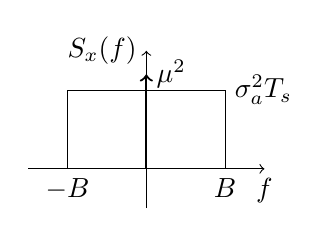
\begin{tikzpicture}
            \draw [->] (-1.5,0) -- (1.5,0) node [anchor=north] {$f$};
            \draw [->] (0,-0.5) -- (0,1.5) node [anchor=east] {$S_x(f)$};
            \draw (-1,0) node [anchor=north] {$-B$} -- (-1,1) -- (1,1) node [anchor=west] {$\sigma_a^2 T_s$} -- (1,0) node [anchor=north] {$B$};
            \draw [thick,->] (0,0) -- (0,1.2) node [anchor=west] {$\mu^2$};
        \end{tikzpicture}
        \endpgfgraphicnamed\end{minipage}
    \end{center}
    La potencia media de señal a la salida del canal es
     \[
     \langle x ^2 \rangle = \int_{-\infty}^\infty S_x(f)\d f =
     \mu^2 + \sigma_a^2 T_s 2B = \mu^2 + \sigma_a^2 = E[a_k^2].
     \]
     Notar que como $\|p\|^2 = \int_{-\infty}^\infty |\hat{P}(f)|^2 \d f = T_s$ se verifica en particular para este caso la f\'ormula
     anunciada en la sección anterior,
     \[\langle x^2 \rangle = E[a_k^2] \|p\|^2 f_s = \overline{E_p}
     f_s.\]
    $x(t)$ llega contaminada de ruido blanco. Resulta entonces
    natural en este caso proceder  como en el caso analógico, y poner como
    filtro de recepción simplemente un pasabajos ideal $[-B,B]$,
    que rechaza al ruido fuera de banda. Notar que:
    \begin{itemize}
    \item La señal de recepci\'on sigue intacta, $p_R(t) = p(t)$, es decir no hay ISI en la detecci\'on.
    \item El ruido de recepción tiene $\sigma^2=\eta B = \frac{\eta f_s}{2}$.
    \end{itemize}
%

    Calculamos ahora expresiones para la probabilidad de error de detección $P_e$ en términos de parámetros físicos del
    canal, para las codificaciones de línea polar o unipolar.

    \begin{description}
        \item[Caso polar binario] $a_k=\pm A$, umbral \'optimo
        $A_0=0$, $\langle x^2 \rangle = A^2$.
        \[ \Rightarrow \ \ P_e = Q\left(\frac{A}{\sigma}\right) = Q\left(\sqrt{\frac{\langle x^2 \rangle}{\sigma^2}}\right) = Q\left(\sqrt{\frac{S}{N}}\right).\]
        que es la misma expresión que obtuvimos con pulsos NRZ.

        Otra expresión (más fácil de generalizar): sea $\overline{E}_p$ la energía media del pulso $a_k
        p(t)$,
        en este caso $\overline{E}_p = E[a_k^2]\|p\|^2 = A^2 T_s$.
                \[\left.\begin{gathered}
                        A^2 = S = \overline{E}_p f_s\\
                        \sigma^2 = N = \eta \frac{f_s}{2}
                      \end{gathered}\right\}\Rightarrow \frac{S}{N} = \frac{2\overline{E}_p}{\eta}\Rightarrow \col{P_e = Q\left(\sqrt{\frac{2\overline{E}_p}{\eta}}\right)}\]
        que depende solo de parámetros físicos del canal:
        \begin{itemize}
            \item Energía media del pulso.
            \item Densidad espectral de ruido.
            \item ¡No depende de $f_s$!
        \end{itemize}
        \vspace{1ex}

        \item[Caso unipolar binario] $a_k = \{0,A\}$, umbral \'optimo
        $A_0=\frac{A}{2}$, $\langle x^2 \rangle = S = \frac{A^2}{2}$.
       % Entonces $S_x(f) = \sigma^2 f_s |\hat{P}(f)|^2 + \mu^2 f_s^2 \hat{P}(f)^2 = \frac{A^2}{4} T_s p_{[-\frac{f_s}{2},\frac{f_s}{2}]}(f) + \frac{A^2}{4}\delta(f)$
        \begin{align*}
 %           S = \langle x^2 \rangle = \frac{A^2}{4} + \frac{A^2}{4} = \frac{A^2}{2}\\
         \sigma^2 = N = \eta \frac{f_s}{2} \Longrightarrow   P_e = Q\left(\frac{A}{2\sigma}\right) =
         Q\left(\frac{1}{\sqrt{2}}\sqrt{\frac{S}{N}}\right).
        \end{align*}

        También aqúi tenemos $\frac{S}{N} = \frac{2\overline{E}_p}{\eta}$
%        \overline{E}_p = E[a_k^2] \int p(t)^2\d t = \frac{A^2}{2} T_s\Rightarrow S = \overline{E}_p T_s$, $N=\frac{\eta f_s}{2}$
        \[\Rightarrow \col{P_e = Q\left(\sqrt{\frac{\overline{E}_p}{\eta}}\right)}\]
        que es menos eficiente que el caso polar.
    \end{description}

\newpage


    \item \textbf{Pulsos de Nyquist de exceso de ancho de banda $\alpha$.}
    \label{item:2}
    Para que estos pulsos pasen intactos por el canal, se require
    la relación $f_s (1+\alpha) \leq 2B$, más restrictiva que la
    anterior. Suponiendo que esto ocurre, podemos usar la misma
    estrategia para elegir el filtro: dejar el pulso intacto,
    eliminar el ruido fuera de banda. Por tanto,
 \[
\Rightarrow \sigma^2 = \frac{\eta f_s}{2}(1+\alpha).
\]
Aquí no buscamos expresiones en términos de $\frac{S}{N}$, en
particular la f\'ormula sencilla para la potencia de la señal PAM
no se aplica. Generalizamos las expresiones para la probabilidad
de error en términos de $\frac{\overline{E}_p}{\eta}$. La energía
media del pulso es
    \[\overline{E}_p = E[a_k^2] \int p(t)^2\d t = E[a_k^2] T_s \left(\underbrace{\frac{1}{T_s}\int |\hat{P}(f)|^2\d f}_{\text{llamamos }\beta}\right)
     = \beta E[a_k^2] T_s.\]
    Se puede verificar (usando la desigualdad de Cauchy-Schwarz) que el parámetro $\beta$ cumple  $\frac{1}{1+\alpha} \leq \beta \leq
    1$.

    Para el caso polar binario, $\overline{E}_p = \beta A^2 T_s\Rightarrow A=\sqrt{\overline{E}_p \frac{f_s}{\beta}}$. $\sigma=\sqrt{\dfrac{\eta f_s}{2} (1+\alpha)}$.

    \[\Rightarrow P_e = Q\left(\frac{A}{\sigma}\right) = Q\left(\sqrt{\frac{2\overline{E}_p}{\eta (1+\alpha)\beta}}\right).\]
    Se agregó un factor $\beta(1+\alpha)\geq 1$ en el denominador,
    respecto del caso de pulsos de Nyquist ideales. Esto deteriora
    $P_e$. Lo mismo ocurre en el caso unipolar.

    Intuitivamente: tuvimos que ensanchar el filtro para dejar pasar la señal y no introducir ISI, pero esta no tiene ``tanta fuerza'' en la parte alta de la banda.

    \item \textbf{Caso de pulsos rectangulares RZ o NRZ}
    \label{item:3}

    Supongamos que el canal tiene $B$ grande y los pulsos $p(t)$ llegan esencialmente rectangulares, ¿qué hago con $H_R$? El dilema es:
    \begin{itemize}
        \item Filtro muy ancho, no deforma pulsos pero pasa mucho ruido a la etapa de
        detecci\'on.
        \item Filtro angosto, reduce el ruido pero deforma los pulsos, introduce ISI.
    \end{itemize}
    Para este tipo de pulsos la estrategia de ``dejarlos pasar intactos'', que tomamos de la comunicación analógica, no
    es la apropiada.
    En realidad, aqu\'i no importa dejar la onda intacta sino lograr la máxima amplitud en el momento del
    muestreo, en relaci\'on al ruido. La optimización del filtro de
    detecci\'on para estos fines se verá a continuación.
\end{enumerate}

%\section{Detección óptima, filtro acoplado}

Replanteamos el problema del diseño del filtro de recepción $H_R$
(denotado aquí por $H$) buscando la mínima probabilidad de error
debida al ruido, ignorando por ahora la ISI. En vez de ``dejar
pasar'' la señal, permitimos que el pulso se distorsione en el
filtro; el objetivo es que en el momento de muestreo el pulso de
salida tenga amplitud máxima en relación al ruido.

Supongamos que a la entrada de $H$ llega un pulso $a_0 p(t)$,
contaminado con ruido blanco $\frac{\eta}{2}$. Aquí $a_0$ puede
ser unipolar ($\{0,A\}$) o polar ($\pm A$), y el pulso de energía
finita tiene forma conocida pero arbitraria.

A la salida del filtro de respuesta impulsiva $h(t)$  y respuesta
en frecuencia $\hat{H}(f)$, tendremos $a_0 p(t) \ast h(t) + n(t)$
donde $n(t)$ es un ruido de media $0$, varianza
$\sigma^2=\frac{\eta}{2}\displaystyle{\int_{-\infty}^{+\infty}
|\hat{H}(f)|^2\d f}$.



Muestreo en $t=\tau$. La señal muestreada es $a_0(p\ast h)
(\tau)$, que toma valores ($\{0,A'\}$) o ($\pm A'$), siendo
$A'=A(p\ast h)(\tau)$. La probabilidad de error de detección $P_e$
estará entonces determinada por la relación $\frac{A'}{\sigma}$,
expresamos su cuadrado a continuación:
%
\[\left(\frac{A'}{\sigma}\right)^2 = \frac{2 A^2 |(p\ast
h)(\tau)|^2}{\eta \int_{-\infty}^{+\infty} |\hat{H}(f)|^2\d f}.\]
Buscamos maximizar lo anterior (para minimizar $P_e$) pero esto no
es inmediato ya que el filtro $H$ aparece en el numerador y
denominador. Para llegar a una expresión más clara escribimos
numerador en términos de la transformada de Fourier $\hat{H}(f)$.

\begin{gather*}
    (p\ast h) \stackrel{\mathcal{F}}{\longrightarrow} \hat{P}(f) \hat{H}(f)\\
    \Rightarrow (p\ast h)(\tau) = \int_{-\infty}^{+\infty} \hat{P}(f)
\hat{H}(f) \e^{j2\pi f \tau}\d f.
\end{gather*}

\paragraph{Llegamos al siguiente problema de optimización:}

\begin{equation}
    \label{eq:op}
    \max_{\hat{H}(f)} \frac{\left|\displaystyle\int_{-\infty}^{+\infty}
\hat{P}(f) \hat{H}(f) \e^{j2\pi f \tau}\d
f\right|^2}{\displaystyle\int_{-\infty}^{+\infty} |\hat{H}(f)|^2\d
f}. \tag{*}
\end{equation}

Como la optimización tiene $\infty$ grados de libertad
(optimización en todos los filtros) no es de solución obvia. Sin
embargo se la puede resolver recurriendo a la desigualdad de
Cauchy-Schwarz (válida para toda función de cuadrado integrable):
%con igualdad $\Leftrightarrow \hat{V} = K \hat{W}$):
\[\left|\left\langle\hat{V}(f),\hat{W}(f)\right\rangle\right|^2 \leq ||\hat{V}||^2
||\hat{W}||^2, \quad \text{ con igualdad }\Leftrightarrow \hat{V}
= K \hat{W}.\] O sea:
\[\left|\int \hat{V}(f) \overline{\hat{W}(f)}\d f\right|^2\leq \int_{-\infty}^{+\infty}
|\hat{V}(f)|^2\d f \int_{-\infty}^{+\infty} |\hat{W}(f)|^2\d f.\]
Tomemos aquí $\hat{V}(f) = \hat{H}(f)$, $\overline{\hat{W}(f)} =
\hat{P}(f)\e^{j2\pi f \tau}$. Usando la desigualdad tenemos
%
\[
\frac{\left|\displaystyle\int_{-\infty}^{+\infty} \hat{P}(f)
\hat{H}(f) \e^{j2\pi f \tau}\d
f\right|^2}{\displaystyle\int_{-\infty}^{+\infty} |\hat{H}(f)|^2\d
f} = \frac{\left|\left\langle
\hat{V},\hat{W}\right\rangle\right|^2}{||\hat{V}||^2}\leq
||\hat{W}||^2 = \int_{-\infty}^{+\infty} |\hat{P}(f)|^2\d f =
||p||^2.\]
O sea que el máximo en \eqref{eq:op} es acotado, y la
igualdad se alcanza sólo si
\[\hat{H}(f) = K\overline{\hat{P}(f)}\e^{-j2\pi f \tau} \Rightarrow h(t)=K
p\left(-(t-\tau)\right)\Rightarrow \col{h(t) = K p(\tau-t)}.\]

\begin{figure}[htb]
    \centering\begin{minipage}{\textwidth}
    \bpgf{Imagenes/filAc/filAc-1}
    \begin{tikzpicture}
        \draw[->] (-0.5,0) -- (4,0) node [anchor=north] {$t$};
        \draw[->] (0,-0.5) -- (0,1.5);
        \draw (0,0) -- (2,1) -- (3,0);
        \path (5,1) node {$\Rightarrow$};
        \begin{scope}[shift={(6,0)}]
                \draw[->] (-0.5,0) -- (4,0) node [anchor=north]
{$t$};
                \draw[->] (0,-0.5) -- (0,1.5) node [anchor=west]
{$h_{opt} = K p(\tau - t)$};
                \draw (0.5,0) -- (1.5,1) -- (3.5,0) node
[anchor=north] {$\tau$};
        \end{scope}
    \end{tikzpicture}
    \endpgfgraphicnamed\end{minipage}
\end{figure}
\FloatBarrier

Concluimos que la respuesta impulsiva del filtro \'optimo tiene la
forma del pulso incidente, invertido en el tiempo: se dice que el
filtro \'optimo est\'a {\bf acoplado (o apareado)}  al pulso.

Para interpretar el resultado en el dominio del tiempo, conviene
escribir el pulso de salida $p_R =h\ast p$ para el filtro
\'optimo:
\begin{align*}
            p_R(t) = (h\ast p) (t)  & = \int_{-\infty}^{+\infty}
h(t-\sigma) p (\sigma)\d \sigma\\
                        & =
%\frac{1}{||p||^2}
K \int_{-\infty}^{+\infty} p(\tau - t + \sigma) p (\sigma)\d
\sigma \\ & = K r_p(t - \tau).
        \end{align*}
Aquí $r_p(\cdot)$ es la autocorrelaci\'on del pulso como señal de
cuadrado integrable. Como la autocorrelación es máxima en cero, el
pulso de salida toma su amplitud máxima en el instante de muestreo
$t=\tau$. En otras palabras: el detector basado en este filtro y
muestreo en $t=\tau$ est\'a {\em correlacionando} la señal de
entrada $a_0 p(t) + n(t)$ con la forma de onda conocida del pulso.


\begin{remarksSN}
    $\phantom{1}$
    \begin{enumerate}
        \item La constante $K$ es arbitraria, escalar el filtro no
        cambia el cociente de \eqref{eq:op}. Una elección cómoda es
$K=\dfrac{1}{||p||^2}=\dfrac{1}{r_p(0)}$: de ese modo el pulso de
salida $p_R(t)$ tiene valor m\'aximo igual a 1, alcanzado en
$t=\tau$. En ese caso la amplitud $A'$ de muestreo coincide con la
amplitud $A$ de los s\'imbolos de entrada.
        \item $\tau$ sería idealmente arbitrario, excepto que en la
práctica queremos $h(t)$ causal. Entonces tomo $\tau$ igual a la
duración del pulso $p(t)$ (si $p(t)=\sinc$ hay que truncarlo).
    \end{enumerate}
\end{remarksSN}

El máximo de nuestro problema de optimización es $\|p\|^2$. Por
tanto tenemos
\[
\left(\dfrac{A'}{\sigma}\right)^2_{\text{max}} = 2
\frac{A^2}{\eta} ||p||^2.\]
% Los libros tienen una generalización para ruido coloreado, $S_n(f)$.

A partir de esta fórmula podemos escribir la probabilidad de error
en términos de la energía media del pulso recibido,
$\overline{E}_p = E[a_k^2] ||p||^2$, en los distintos casos.

\begin{description}
    \item[Polar binario]
    \[\overline{E}_p = A^2 ||p||^2 \Rightarrow
\left(\frac{A'}{\sigma}\right)_\text{max} =
\sqrt{\frac{2\overline{E}_p}{\eta}} \Rightarrow P_e^\text{opt} =
Q\left(\sqrt{2\frac{\overline{E}_p}{\eta}}\right).\]
    \item[Unipolar binario]
    \[\overline{E}_p = \frac{A^2}{2}||p||^2 \Rightarrow
\left(\frac{A'}{\sigma}\right)_\text{max} = 2
\sqrt{\frac{\overline{E}_p}{\eta}} \Rightarrow P_e^\text{opt} =
Q\left(\sqrt{\frac{\overline{E}_p}{\eta}}\right).\]
 \end{description}

Estas fórmulas son iguales a las que obtuvimos para la detección
con pulsos de Nyquist, filtro pasabajos ideal. Esto no es
casualidad: para $p(t) = \sinc(\pi f_s t)$, el filtro acoplado es
un pasabajos ideal. O sea que en ese caso ya hicimos (sin saberlo)
lo óptimo. Pero las fórmulas valen para cualquier forma de pulso
con su detector apareado.

\subsection*{Caso M-ario polar} Ya se vio anteriormente que aquí la
probabilidad de error de símbolo es $P_e=2\frac{M-1}{M}
Q\left(\frac{A}{\sigma}\right)$. O sea que también aquí debemos
maximizar $\frac{A}{\sigma}$ y por tanto obtenemos el mismo filtro
acoplado. Escribimos la expresión en términos de $\overline{E}_p$
para este caso:
\begin{gather*}
 E[a_k]^2 = \frac{A^2 (M^2-1)}{3} \Rightarrow \overline{E}_p = A^2 \frac{(M^2-1)}{3}||p||^2
\Rightarrow \left(\frac{A'}{\sigma}\right)^2_{max} = \frac{6 \bar{E}_p}{\eta (M^2-1)}\\
\Rightarrow {\col{P_e^{opt} = 2\frac{M-1}{M}
Q\left(\sqrt{\frac{6\bar{E}_p}{\eta(M^2-1)}}\right)}}
\end{gather*}

\subsection*{Detector acoplado para pulsos rectangulares}

Tomemos por ejemplo los pulsos NRZ, $p(t) = p_{[0,T_s]}(t)$. El
filtro acoplado tendrá la respuesta impulsiva (tomando
$\tau=T_s$):
\[
\Rightarrow h(t) = \dfrac{1}{||p||^2} p(T_s-t) =
\dfrac{1}{T_s}p(t).
\]
\begin{minipage}{0.6\textwidth}
 A la salida del filtro se obtiene el pulso triangular
 \[p_R(t)=h(t)\ast p(t). \]
\end{minipage}
\begin{minipage}{0.4\textwidth}
 \begin{center}
  \bpgf{Imagenes/filAc/filAc-2}
    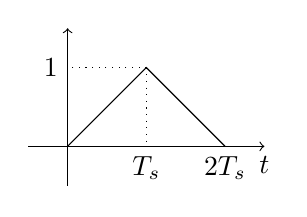
\begin{tikzpicture}
      \draw [->] (-0.5,0) -- (2.5,0) node [anchor=north] {$t$};
      \draw [->] (0,-0.5) -- (0,1.5);
      \draw (0,0) -- (1,1) -- (2,0) node [anchor=north] {$2T_s$};
      \draw [dotted] (1,1) -- (0,1) node [anchor=east] {$1$};
      \draw [dotted] (1,1) -- (1,0) node [anchor=north] {$T_s$};
    \end{tikzpicture}
  \endpgfgraphicnamed
 \end{center}
\end{minipage}

El filtro de recepción distorsionó fuertemente el pulso, pero esto
se  hizo de modo de maximizar $\frac{A}{\sigma}$ en el instante de
$t=T_s$ de muestreo.


\subsection*{¿Qué paso con la ISI?}

Al estudiar un solo pulso aislado, no contemplamos este tema.
Veamos:
\begin{itemize}
 \item En el caso pulsos de Nyquist ideales el detector acoplado es un pasabajos ideal, entonces los pulsos pasan intactos,
 sin ISI.
 \item En el caso de pulsos rectangluares NRZ. Vemos que $p_R(k T_s) = 0$ excepto en un valor ($k=1$). Entonces tampoco hay
 ISI.  Simplemente hay un retardo de $\tau = T_s$ al detectar.
 \item  De hecho, cualquier pulso de duración $\leq T_s$ (por ej., RZ) genera una $p_R(t)$ de duración $\leq
 2T_s$, que debidamente muestreado no genera  ISI.
\end{itemize}


\subsection*{Para pulsos de Nyquist con exceso de ancho de banda
$\alpha$}

El detector acoplado tiene respuesta en frecuencia
\begin{gather*}
 \hat{H}(f) = K \overline{\hat{P}(f)} \e^{-j2\pi f\tau}\\
 \Rightarrow \hat{P}_R = \hat{H}\hat{P} = K |\hat{P}(f)|^2 \e^{-j2\pi f \tau}
\end{gather*}
El último término es un retardo, afecta sólo el instante de
muestreo. A efectos de estudiar la ISI podemos tomar $P_R(f) =
K|\hat{P}(f)|^2$.
\begin{figure}[htb]
 \begin{center}\begin{minipage}{\textwidth}
  \bpgf{Imagenes/filAc/filAc-3}
  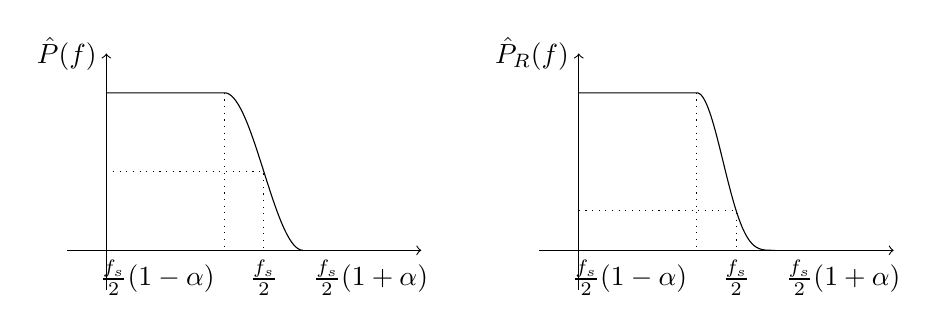
\begin{tikzpicture}
    \draw [->] (-0.5,0) -- (4,0);
    \draw [->] (0,-0.5) -- (0,2.5) node [anchor=east] {$\hat{P}(f)$};
    \draw  (0,2) -- (1.5,2) -- plot  [domain=1.5:2.5,samples=200] (\x,{cos(pi*(\x-1.5) r)+1});
    \draw [dotted] (1.5,2) -- (1.5,0) node [below left] {$\frac{f_s}{2}(1-\alpha)$};
    \draw [dotted] (0,1) -- (2,1) -- (2,0) node [below] {$\frac{f_s}{2}$};
    \path (2.5,0) node [below right] {$\frac{f_s}{2}(1+\alpha)$};
    \begin{scope}[shift={(6,0)}]
    \draw [->] (-0.5,0) -- (4,0);
    \draw [->] (0,-0.5) -- (0,2.5) node [anchor=east] {$\hat{P}_R(f)$};
    \draw  (0,2) -- (1.5,2) -- plot  [domain=1.5:2.5,samples=200] (\x,{(cos(pi*(\x-1.5) r)+1)^2/2});
    \draw [dotted] (1.5,2) -- (1.5,0) node [below left] {$\frac{f_s}{2}(1-\alpha)$};
    \draw [dotted] (0,0.5) -- (2,0.5) -- (2,0) node [below] {$\frac{f_s}{2}$};
    \path (2.5,0) node [below right] {$\frac{f_s}{2}(1+\alpha)$};
    \end{scope}
   \end{tikzpicture}
   \endpgfgraphicnamed\end{minipage}
 \end{center}

\end{figure}

$|\hat{P}(f)|^2$ no tiene simetría, entonces no cumple la condición de ISI nula.

O sea: poner el filtro óptimo desde el punto de vista del ruido,
me complica la ISI.

\newpage    %%% Solo para compilacion global.

Alternativas:
\begin{enumerate}
 \item En vez del $H_{opt}$, poner un pasabajos $(1+\alpha)\frac{f_s}{2}$, como ya se estudió. La $P_e$ da un poco peor,
 pero no introduzco ISI que sería más grave.
 \item Sabiendo que va a haber un filtro apareado, diseño $\hat{P}(f)$ para que $|\hat{P}(f)|^2$ no tenga ISI.
 Se usa a veces el pulso de {\bf raíz de coseno alzado.}
\end{enumerate}

%%%\newpage %% Va para compilar solo la parte digital
%% No va para el compilado global


\subsection*{Resumen: comunicación digital banda base}
\begin{figure}[htb]
    \centering
    \resizebox{\textwidth}{!}{%
    \bpgf{Imagenes/digBB/digBB-1}
    \begin{blockdiagram}
        \matrix[row sep=5mm, column sep=10mm]{
            & & \node[etiqueta] (ruido) {\large ruido blanco, $\frac{\eta}{2}$}; & & & & & \node[punto] (p1) {}; & \node [punto] (p2) {};\\
            \node[etiqueta] (inicio) {\large  $\sum_k a_k p_T(t-kT_s)$}; %& \node[block] (pulso) {$P_T(t)$};
             & \node[block] (canal) {\large CANAL} node[above=3mm] {
                    \begin{minipage}{2.2cm}
                       \large  (ancho de banda $B$)
                    \end{minipage}};
            & \node[operator] (sum) {$+$}; & \node [block] (filtro) {\large $\hat{H}_R(f)$} node [below=5mm] {
            \begin{minipage}{2.5cm}
                FILTRO DE\\RECEPCI�N
                \end{minipage}};
            & \node[punto] (p3) {} node [anchor=south] {\large $x_R(t)+n(t)$}; & \node [punto] (p4) {}; & & & \node[punto] (p5) {}; & \node [draw, isosceles triangle,thick] (comp) {
            \begin{minipage}{5mm}
                $+$\\$-$
            \end{minipage}};
            & \node[etiqueta] (salida) {\large $\{\hat{a}_k\}$};\\
            & & & & & & \node[block] (sinc) {\large SINCR}; & & \node [etiqueta] (v0) {$A_0$};\\
        };
        \draw [-stealth] (inicio) -- (canal);
        \draw [-stealth] (canal) -- (sum);
        \draw [-stealth] (ruido) -- (sum);
        \draw [-stealth] (sum) -- (filtro);
        \draw (filtro) -- (p3) -- (p4) -- (p2);
        \draw [-stealth] (p3) |- (sinc);
        \draw [-stealth] (sinc) -| (p1);
        \draw [-stealth] (p5) |- (comp.150);
        \draw [-stealth] (v0) |- (comp.south west);
        \draw [-stealth] (comp) -- (salida);
    \end{blockdiagram}
\endpgfgraphicnamed

    }
\end{figure}
\FloatBarrier

\begin{itemize}
 \item Transmito sucesión de pulsos $\sum a_k p_T(t-kT_s)$ (PAM)
 \item El canal introduce 2 distorsiones
\begin{enumerate}
  \renewcommand{\theenumi}{\roman{enumi}}
  \item \label{itemRes:1}Forma del pulso, por filtrado. Puede causar ISI.

  \item \label{itemRes:2}Ruido blanco.
\end{enumerate}
\end{itemize}

Si nos concentramos en (\ref{itemRes:1}), elegimos un pulso de
Nyquist y/o colocamos un \emph{ecualizador} en $\hat{H}_R(f)$.

Si nos concentramos en (\ref{itemRes:2}), ponemos en
$\hat{H}_R(f)$ el \emph{detector acoplado}.

Hay dos casos extremos en que las dos funciones se realizan
simultaneamente:

\begin{itemize}
 \item $p(t) = \sinc(\pi f_s t)$ (Nyquist ideal), $\hat{H}_R(f)$ pasabajos ideal. Se aplica a la situación:
    \begin{itemize}
     \item canal con $B$ muy restrictiva.
     \item puedo implementar la complejidad de pulsos/filtro.
    \end{itemize}
 \item $p(t)$ rectángular NRZ o RZ. Detector acoplado: $h_R(t) = \frac{1}{T_s}p(t)$. Se aplica a la situación:
\begin{itemize}
 \item $B$ muy grande (respecto a $f_s$).
  \item Implementación más simple. Sobre todo, el amplificador de transmisión puede ser no lineal.
\end{itemize}
\end{itemize}

En otros casos, puede existir conflicto entre los objetivos de
combatir las distorsiones (\ref{itemRes:1}) y (\ref{itemRes:2}).
Por ejemplo se vio que esto ocurría al usar pulsos de Nyquist con
exceso de ancho de banda. Aquí o se realiza un diseño conjunto de
$p_T$, $\hat{H}_R$, o sino se acepta una detección subóptima
respecto al ruido.

%\section{Repetidores y regeneración}

Supongamos se transmite una onda digital de banda base por un
cable largo. Al propagarse la onda se introduce atenuación, que
debe compensarse por amplificación posterior. Una estrategia
comúnmente usada es dividir el cable en tramos y amplificar en
cada tramo. Ejemplo de uso: cajas subterráneas en telefonía.

\begin{figure}[htb]
 \begin{center}\begin{minipage}{\textwidth}
  \bpgf{Imagenes/repReg/repReg-1}
  \begin{blockdiagram}
    \matrix[row sep=5mm, column sep=10mm]{
        & \node[etiqueta] (ruido1) {$n_1$}; & & \node[etiqueta] (ruido2) {$n_2$}; & & & \node[etiqueta] (ruidom) {$n_m$};\\
        \node[etiqueta] (inicio) {$x(t)$}; & \node[operator] (sum1) {$+$}; & \node[block] (amp1) {AMP}  node [above right=5mm] {$y_1(t)$} node [below=3mm] {\begin{minipage}{1.5cm}\centering ganancia\\ $\frac{1}{a}$\end{minipage}}; & \node[operator] (sum2) {$+$}; & \node[block] (amp2) {AMP}; & \node[etiqueta] (puntos) {$\ldots$}; & \node[operator] (summ) {$+$}; & \node[block] (ampm) {AMP}; & \node[etiqueta] (salida) {$y(t)$};\\
    };
    \draw [->,ultra thick] (inicio) -- node [anchor=north] {\begin{minipage}{20mm}\centering TR.1\\ atenuación $a$ ($a\ll 1$)\end{minipage}} (sum1);
    \draw [->] (sum1) -- (amp1);
    \draw [->] (ruido1) -- (sum1);
    \draw [->,ultra thick] (amp1) -- node [anchor=north] {TR. 2} (sum2);
    \draw [->] (ruido2) -- (sum2);
    \draw [->] (sum2) -- (amp2);
    \draw [->,ultra thick] (amp2) -- (puntos);
    \draw [->,ultra thick] (puntos) -- (summ);
    \draw [->] (ruidom) -- (summ);
    \draw [->] (summ) -- (ampm);
    \draw [->] (ampm) -- (salida);
  \end{blockdiagram}
  \endpgfgraphicnamed\end{minipage}
 \end{center}

\end{figure}
\FloatBarrier

Suponemos que cada etapa tiene ruido aleatorio de varianza
$E[n_i^2] = \sigma^2$.

\[y_1 = \frac{1}{a}(a x + n_1) = x+ \frac{n_1}{a} \qquad \Longrightarrow \left(\frac{S}{N}\right)_1 =
\frac{\langle x^2 \rangle}{\frac{\langle n_1^2\rangle}{a^2}} = a^2
\frac{\langle x^2\rangle}{\sigma^2}.\]

Para la segunda etapa:
\[y_2 = \frac{1}{a}(a y_1 +n_2) = y_1 + \frac{n_2}{a} = x + \frac{n_1+n_2}{a}.\]

Por el mismo razonamiento,
\[y(t) = y_m(t) = x(t) + \frac{n_1+n_2+\cdots+n_m}{a}.\]

\begin{align*}
 \left(\frac{S}{N}\right)_m & = \frac{\langle x^2 \rangle}{\frac{1}{a^2} E\left[(n_1+n_2+\cdots+n_m)^2\right]} =
  \frac{a^2 \langle x^2\rangle}{m \sigma^2}, \qquad \text{suponiendo ruidos independientes.}
%\Rightarrow                   & =
\end{align*}
\[{\col{ \left(\frac{S}{N}\right)_m = \frac{1}{m}
\left(\frac{S}{N}\right)_1}}\]

 Vemos que la relación señal-ruido se degrada linealmente en $m$. Por lo tanto
la $P_e$ se degrada fuertemente (por ejemplo,
$P_e=Q\left(\sqrt{\frac{S}{N}}\right)$ para el caso polar, con
pulsos ideales).

\begin{ejemplo}[numérico] Señal polar, $\left(\frac{S}{N}\right)_1 = 100 \  (20\,dB)$, $m=20$
repetidores.
  \[ \Rightarrow \left(\frac{S}{N}\right)_m = 5 \Rightarrow P_e  = Q(\sqrt{5}) = 1.29\cdot 10^{-2}, \quad\text{muy alto.}\]
 \end{ejemplo}

\subsection*{Repetidor regenerativo}

En vez de solo amplificar (señal y ruido), realiza una detección y
regenera la señal PAM. Sea $p$ la probabilidad de error de una
etapa, $p=Q\left(\sqrt{\left(\frac{S}{N}\right)_1}\right)$.

Suponemos $p\ll 1$ y errores independientes en cada etapa.
Calculamos la probabilidad de error de $m$ etapas. Notar que
\[1 - P_e(m\text{ etapas})  = (1-P_e(1 \text{ etapa}))^m \]
(es decir, para no tener errores en un símbolo exijo no tenerlos
en ninguna de las $m$ detecciones independientes). Por tanto
\[P_e(m\text{ etapas}) = 1 -(1-p)^m  \approx 1-(1-mp) = mp.\]
En este caso, $P_e$ se deteriora linealmente con $m$.

Volviendo al ejemplo, $p=Q(10) = 7.7\cdot 10^{-24}$ para una
etapa, por tanto
\[ P_e (20 \text{ etapas}) \approx 20 p = 1.5\cdot 10^{-22},\]
muchísimo más bajo que en el caso no regenerativo.

\paragraph{Moraleja}$\phantom{1}$
\begin{itemize}
 \item Es mejor regenerar.
 \item Esta es una de las mayores ventajas de la comunicación digital por sobre la analógica.
\end{itemize}


\chapter{Modulación Digital Pasabanda}\label{chapter:modulacion pasabanda}
%\section{Introducción a la Modulación digital pasabanda}

Hasta ahora vimos transmisión de símbolos digitales por pulsos de
banda base, que son apropiados para canales que responden en esas
frecuencias. Por ejemplo, el par trenzado o cable coaxial, usado
en líneas T1 de telefonía.

Muchas veces, hace falta modular datos digitales en otras partes del espectro, por ejemplo:
\begin{enumerate}
    \item Modems para el canal telefónico de voz, que no responde en continua.
    \item Enlaces de radio microondas entre dos torres
    \item Telefonia celular.
\end{enumerate}

\noindent En principio, una solución posible sería modular en
forma analógica una onda digital de banda base:

\begin{figure}[htb]
    \centering\begin{minipage}{\textwidth}
    \bpgf{Imagenes/MDPasa/MDPasa-1}
    \begin{blockdiagram}
        \matrix[row sep=5mm, column sep=10mm]{
            \node[etiqueta] (inicio) {\parbox{2cm}{\centering fuente digital\\$\{a_k\}$}}; & \node [block] (modD) {\parbox{2cm}{MODUL\\DIGITAL}}; & \node [block] (modA) {\parbox{2cm}{MODUL\\ANALOG.}};\\
            & & & \node [block] (canal) {\parbox{2.5cm}{\centering CANAL\\PASABANDA}};\\
            \node[punto] (salida) {}; &\node [block] (detD) {\parbox{2.5cm}{DETECCIÓN\\DIGITAL}}; & \node[block] (detA) {\parbox{2cm}{DEMOD.\\ANALOG.}};\\
        };
        \draw [->] (inicio) -- (modD);
        \draw [->] (modD) -- node [below=12mm] {$\sum a_k p(t-kT_s)$} (modA);
        \draw [->] (modA) -| (canal);
        \draw [->] (canal) |- (detA);
        \draw [->] (detA) -- (detD);
        \draw [->] (detD) -- (salida);
    \end{blockdiagram}
    \endpgfgraphicnamed\end{minipage}
\end{figure}
\FloatBarrier

Esto es conceptualmente correcto, pero no necesariamente lo más eficiente. Puede
convenir combinar los bloques de arriba y los de abajo, aprovechando el hecho de que transmito señales ``especiales'' de
banda base. En particular para la detección, el objetivo es identificar el símbolo enviado, para cual no hace
falta demodular fielmente la onda analógica intermedia de banda base.

Para la modulación, esto implica generar directamente una señal
similar a la PAM, pero donde los pulsos de banda base $p(t)$ son
reemplazados por {\em pulsos de radiofrecuencia}, concentrados en
la banda de interés para la comunicación.

\newpage

Las siguientes figuras muestran ejemplos de este tipo, en comparación con el caso de banda base.
En cada caso, la amplitud (ASK), fase (PSK) o frecuencia (FSK) del pulso se utiliza para codificar el
símbolo, que en estos casos es binario.

\begin{figure}[htb]
    \centering
    \resizebox{\textwidth}{!}{
    \bpgf{Imagenes/MDPasa/MDPasa-2}
    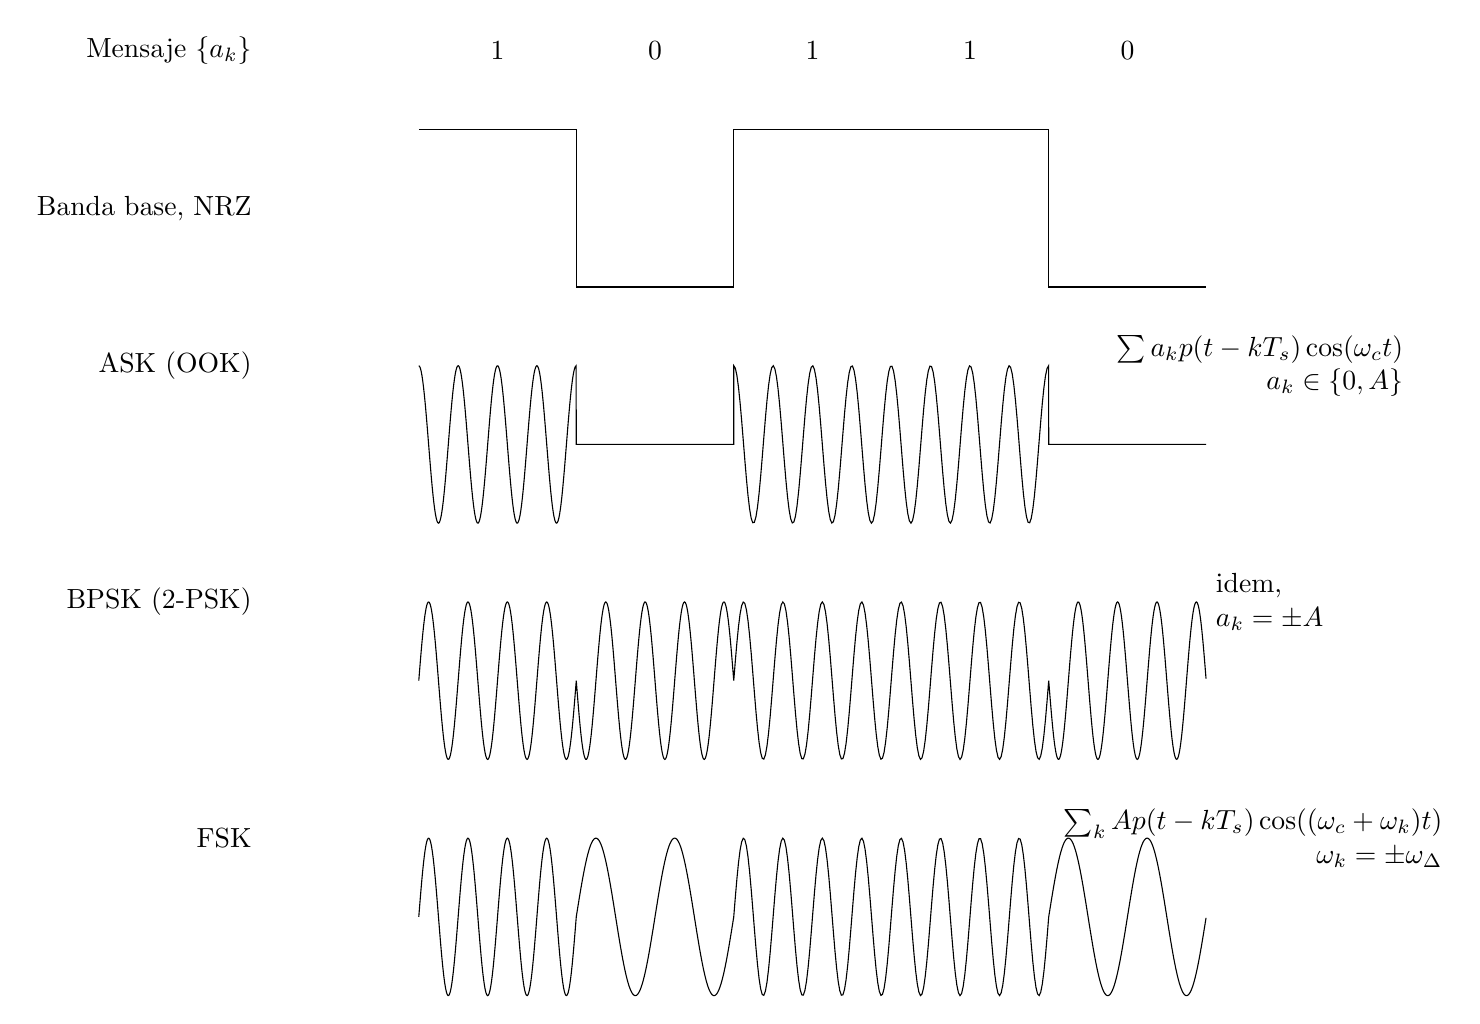
\begin{tikzpicture}
        \path (-2,1) node [anchor=east] {Mensaje $\{a_k\}$};
        \path (1,1) node {$1$} -- (3,1) node {$0$} -- (5,1) node {$1$} -- (7,1) node {$1$} -- (9,1) node {$0$};
        \begin{scope}[shift={(0,-2)}]
            \path (-2,1) node [anchor=east] {Banda base, NRZ};
            \draw (0,2) -- (2,2) -- (2,0) -- (4,0) -- (4,2) -- (8,2) -- (8,0) -- (10,0);
        \end{scope}
        \begin{scope}[shift={(0,-4)}]
            \path (-2,1) node [anchor=east] {ASK (OOK)};
            \draw [samples=200,domain=0:2] plot (\x,{cos(4*pi*\x r)}) -- (2,0) -- (4,0) -- plot [samples=200,domain=4:8] (\x,{cos(4*pi*\x r)}) -- (8,0) -- (10,0);
            \path (10,1) node {\parbox{5cm} {\raggedleft $\sum a_k p(t-kT_s)\cos(\omega_ct)$\\$a_k\in\{0,A\}$}};
        \end{scope}
        \begin{scope}[shift={(0,-7)}]
            \path (-2,1) node [anchor=east] {BPSK (2-PSK)};
            \draw [samples=200,domain=0:2] plot (\x,{sin(4*pi*\x r)}) -- plot [domain=2:4] (\x,{-sin(4*pi*\x r)}) -- plot [samples=200,domain=4:8] (\x,{sin(4*pi*\x r)}) -- plot [domain=8:10] (\x,{-sin(4*pi*\x r)});
            \path (10,1) node [anchor=west] {\parbox{2.5cm}{idem,\\$a_k = \pm A$}};
        \end{scope}
       \begin{scope}[shift={(0,-10)}]
            \path (-2,1) node [anchor=east] {FSK};
            \draw [samples=200,domain=0:2] plot (\x,{sin(4*pi*\x r)}) -- plot [domain=2:4] (\x,{sin(2*pi*\x r)}) -- plot [samples=200,domain=4:8] (\x,{sin(4*pi*\x r)}) -- plot [domain=8:10] (\x,{sin(2*pi*\x r)});
%            \path (10,1) node [anchor=west] {\parbox{2.5cm}{fórmula\\después}};
            \path (10,1) node {\parbox{6cm}{\raggedleft $\sum_k A p(t-kT_s) \cos ((\omega_c  + \omega_k) t)$ \\ $\omega_k = \pm \omega_\Delta$ }};
        \end{scope}
    \end{tikzpicture}
    \endpgfgraphicnamed
    }
\end{figure}
\FloatBarrier
%
Los casos de ASK y BPSK corresponden a modulación lineal, es decir
que $x_c$ depende linealmente de los símbolos; en el caso de FSK la dependencia es no lineal.
En los dibujos se utilizó $p(t)$ rectangular, NRZ; también puede pensarse en modular pulsos de
banda base más sofisticados, como los de Nyquist (más dificiles de
dibujar en el tiempo). 
\section{Modulación pasabanda binaria y su espectro de potencia}
%
%Al igual que en el caso de banda base, comenzamos el estudio de estas formas de onda
%analizando la densidad espectral de potencia correspondiente.

\subsection*{Modulación pasabanda binaria lineal}

Consideramos aquí la onda
\[
x_c(t) = \sum_k a_k p(t-kT_s) \cos(\omega_c t),
\]
donde los símbolos $\{a_k\}$ son I.I.D., binarios. Esta se\~nal puede interpretarse
como el resultado de una modulación analógica en banda lateral doble (DSB) aplicado a la onda PAM de banda base $x(t) = \sum_k a_k p(t-kT_s)$.
El caso de ASK corresponde a una onda PAM unipolar, mientras que el de BPSK corresponde a la polar.

\newpage

Podemos utilizar esta identificación para obtener la densidad espectral de potencia de la onda modulada:

\begin{equation}
    \label{eq:dep}
    \col{S_{x_c}(f) = \frac{S_x(f-f_c) + S_x(f+f_c)}{4}}\tag{\#}
\end{equation}

\noindent donde recordamos la expresión para la densidad espectral de potencia en banda base:
\[
S_x(f) = \sigma_a^2 f_s |\hat{P}(f)|^2 + \mu^2 f_s^2 \sum_{n=-\infty}^{+\infty} |\hat{P}(n f_s)|^2\delta(f-nf_s).
\]
Aquí $\mu$ y $\sigma_a^2$ son la media y varianza, respectivamente, de los símbolos I.I.D. $\{a_k\}$, y \\ $\hat{P}(f)$ la
transformada de Fourier del pulso de banda base.


\paragraph{Comentario.} En rigor, para justificar esta fórmula a partir de los procesos estacionarios había que introducir
un retardo aleatorio en la onda PAM, y también para obtener (\ref{eq:dep}) de la modulación DSB se incluía una fase aleatoria.
Ignoramos estos temas de aquí en mas, interpretando las densidades
espectrales en el sentido de las señales determinísticas de
potencia finita.


\subsubsection*{Caso de modulación BPSK}

La onda pasabanda BPSK $x_c(t)$ corresponde a modular una onda PAM de banda base $x(t)$ {\em polar, binaria}, con $a_k=\pm A$. Recordemos que ésta tiene densidad espectral de potencia $S_x(f)= A^2 f_s |\hat{P}(f)|^2$. Bosquejamos la correspondiente $S_{x_c}(f)$ en dos casos particulares.

\begin{minipage}{0.5\textwidth}
\begin{enumerate}
    \item Pulsos de Nyquist con exceso de ancho de banda $\alpha$

    $\hat{P^1}(f) = $\parbox[m]{0.6\textwidth}{\resizebox{0.6\textwidth}{!}{
            \bpgf{Imagenes/MDPasa/MDPasa-5}
            \begin{tikzpicture}
                \draw [-stealth] (-2,0) -- (2,0) node [anchor=north] {$f$};
                \draw [-stealth] (0,-0.5) -- (0,2);
                \draw [samples=200,domain=-1.25:-0.75] plot (\x,{1/2*(1+cos(2*pi*(\x-0.25) r))}) -- (0.75,1);
                \draw [samples=200,domain=0.75:1.25] plot (\x,{1/2*(1+cos(2*pi*(\x+0.25) r))});
                \path (0,1) node [anchor=south west] {$T_s$};
                \draw [dotted] (1,0.5) -- (1,0) node [anchor=north] {$\frac{f_s}{2}$};
                \draw [dotted] (-1,0.5) -- (-1,0) node [anchor=north] {$-\frac{f_s}{2}$};
            \end{tikzpicture}
            \endpgfgraphicnamed}}

    \item Pulsos NRZ, $\hat{P^2}(f) = T_s \sinc (\pi T_s f)$.
\end{enumerate}
\end{minipage}\hfil
\begin{minipage}{0.45\textwidth}
    \resizebox{\textwidth}{!}{
    \bpgf{Imagenes/MDPasa/MDPasa-6}
    \begin{tikzpicture}
        \draw [-stealth] (-0.5,0) -- (8,0) node [anchor=north] {$f$};
        \draw [-stealth] (0,-3.5) -- (0,2) node [anchor=west] {$S^1_{x_c}(f)$};
        \path  (0,-1) node [anchor=west] {$S^2_{x_c}(f)$};
        \begin{scope}[shift={(4,0)}]
                    \draw [samples=200,domain=-1.25:-0.75] plot (\x,{1/2*(1+cos(2*pi*(\x-0.25) r))}) -- (0.75,1);
                    \draw [samples=200,domain=0.75:1.25] plot (\x,{1/2*(1+cos(2*pi*(\x+0.25) r))});
                    \path (0,1) node [anchor=south west] {$A^2\frac{T_s}{4}$};
                    \draw [dotted] (1,0.5) -- (1,0) node [anchor=north] {$f_c+\frac{f_s}{2}$};
        \end{scope}
        \begin{scope}[shift={(0,-3)}]
            \draw [-stealth] (-0.5,0) -- (8,0) node [anchor=north] {$f$};
            \draw [samples=210,domain=0:8] plot (\x,{(sin(pi/2*(\x-4) r)/(pi/2*(\x-4)))^2});
            \path (4,1) node [anchor=south west] {$A^2\frac{T_s}{4}$};
        \end{scope}
        \draw [dotted] (2,1) -- (2,-3) node [anchor=north east] {$f_c-f_s$} -- (2,-3.5);
        \draw [dotted] (6,1) -- (6,-3) node [anchor=north west] {$f_c+f_s$} -- (6,-3.5);
        \draw [dotted] (4,1.5) -- (4,-3) node [anchor=north] {$f_c$};
    \end{tikzpicture}
    \endpgfgraphicnamed}
\end{minipage}

El segundo caso ocupa una banda mucho mayor (en principio,
infinita). En general se utiliza algún criterio práctico que considera un ancho de banda efectivo
para esos casos. Por ejemplo, considerar solamente el ``lóbulo central'' de la densidad espectral,
que tiene $90\%$ de la potencia.
\FloatBarrier

\subsubsection*{Caso ASK, pulsos NRZ}$\phantom{1}$

\begin{figure}[htb]
    \centering\begin{minipage}{\textwidth}
    \bpgf{Imagenes/MDPasa/MDPasa-7}
    \begin{tikzpicture}
        \draw [-stealth] (-0.5,0) -- (8,0) node [anchor=north] {$f$};
        \draw [-stealth] (0,-0.5) -- (0,2.5);
        \draw [-stealth] (-0.5,0) -- (8,0) node [anchor=north] {$f$};
        \draw [samples=210,domain=1:7] plot (\x,{(sin(pi*(\x-4) r)/(pi*(\x-4)))^2});
        \path (4.1,1) node [anchor=west] {$A^2\frac{T_s}{16}$};
        \draw [thick,-stealth] (4,0) node [anchor=north] {$f_c$} -- (4,2) node (a) [anchor=west] {$\left(\frac{A^2}{16}\right)$};
        \node [anchor=west] (b) at (6,2) {\parbox{3cm}{\centering tiene portadora (como AM)}};
        \draw [-stealth] (a) -- (b);
    \end{tikzpicture}
    \endpgfgraphicnamed\end{minipage}
\end{figure}
\FloatBarrier

La combinación de ASK con pulsos de Nyquist es en principio
también posible, pero no de uso práctico ya que ASK se motiva
principalmente por razones de simplicidad.


%\newpage

\subsection*{Modulación FSK binaria}

\begin{minipage}{0.5\textwidth}
\[x_c(t) = \sum_k A p(t-kT_s)\cos (\omega_c t + 2\pi f_k t),\]
donde $f_k=\pm f_\Delta$, y los pulsos son NRZ.
\end{minipage}
\hfil
\begin{minipage}{0.45\textwidth}
    \resizebox{\textwidth}{!}{
    \bpgf{Imagenes/MDPasa/MDPasa-10}
    \begin{tikzpicture}[xscale=1.5]
        \draw [-stealth] (-0.5,0) -- (5,0);
        \draw [-stealth] (0,-1.5) -- (0,1.5);
        \draw [domain=1:2.5,samples=200] plot (\x,{-sin(pi*\x r + 10*pi*\x r)});
        \draw [domain=2.5:4,samples=200] plot (\x,{sin(pi*\x r + 4*pi*\x r)});
        \path (1.75,-1.25) node {$f_c+f_\Delta$};
        \path (3.25,-1.25) node {$f_c-f_\Delta$};
    \end{tikzpicture}
    \endpgfgraphicnamed}
\end{minipage}

Notar que la onda FSK puede verse como la superposición de dos ondas ASK,
una en cada frecuencia, activadas por los símbolos opuestos.
?`Es posible evaluar su espectro de potencia superponiendo los de ASK?
Esto no esta justificado ya que las ondas ASK no son independientes, pero nos
sirve para tener una idea:

\begin{figure}[htb]
    \centering\begin{minipage}{\textwidth}
    \bpgf{Imagenes/MDPasa/MDPasa-11}
    \begin{tikzpicture}[xscale=1.5]
        \draw [-stealth] (-0.5,0) -- (8,0) node [anchor=north] {$f$};
        \draw [-stealth] (0,-0.5) -- (0,2.5);
        \draw [samples=400,domain=1:7] plot (\x,{2*(sin(2*pi*(\x-3) r)/(2*pi*(\x-3)))^2+2*(sin(2*pi*(\x-5) r)/(2*pi*(\x-5)))^2});
        \draw [-stealth,thick] (3,0) node [anchor=north] {$f_c-f_\Delta$} -- (3,2.3);
        \draw [-stealth,thick] (5,0) node [anchor=north] {$f_c+f_\Delta$} -- (5,2.3);
    \end{tikzpicture}
    \endpgfgraphicnamed\end{minipage}
\end{figure}
\FloatBarrier


\noindent La evaluación rigurosa del problema no es sencilla (recordar que tampoco era sencillo evaluar espectros de FM).
Un caso resuelto por Sunde (ver libros) es para
$f_\Delta=\frac{f_s}{2}$. El resultado tiene la forma (\ref{eq:dep}), trasladando el espectro pasabajos

\begin{minipage}{0.6\textwidth}
\begin{align*} S_{x}(f) =& \frac{A^2}{4}\left[\delta(f-\frac{f_s}{2})+\delta(f+\frac{f_s}{2})\right]\\& + \frac{4 A^2 T_s \cos^2(\pi T_s f)}{\pi^2 (4 T_s^2 f^2 - 1)^2}.\end{align*}
\end{minipage}\hfil
\begin{minipage}{0.4\textwidth}
    \resizebox{\textwidth}{!}{
%\begin{figure}[htb]
%    \centering
    \bpgf{Imagenes/MDPasa/MDPasa-12}
    \begin{tikzpicture}[xscale=1.5]
        \draw [-stealth] (-3,0) -- (3,0) node [anchor=north] {$f$};
        \draw [-stealth] (0,-0.5) -- (0,2.5);
        \draw [samples=400,domain=-2.5:2.5] plot (\x,{20*(cos(pi*\x r)/(pi*(4*\x^2-1)))^2});
        \draw [-stealth,thick] (-0.5,0) node [anchor=north] {$-\frac{f_s}{2}$} -- (-0.5,2.3);
        \draw [-stealth,thick] (0.5,0) node [anchor=north] {$\frac{f_s}{2}$} -- (0.5,2.3);
        \draw (-1.5,0.1) -- (-1.5,-0.1) node [anchor=north] {$-3\frac{f_s}{2}$};
        \draw (1.5,0.1) -- (1.5,-0.1) node [anchor=north] {$3\frac{f_s}{2}$};
    \end{tikzpicture}
    \endpgfgraphicnamed}
%\end{figure}
\end{minipage}

%

Concluimos que la onda FSK ocupa un ancho de banda algo mayor que las modulaciones lineales ASK, BPSK, una vez más en
forma consistente con la situación en las modulaciones analógicas correspondientes.




\subsection*{Sobre eficiencia espectral en modulación digital
pasabanda}

Notar que en todas las modulaciones consideradas el ancho de banda
es como mínimo el doble que la correspondiente situación de banda base.
Ello implica que la eficiencia espectral en bps/Hz será la mitad.

Por ejemplo, si usamos BPSK con pulsos ideales de Nyquist, ocupa una banda $f_s$,
y obtiene una eficiencia espectral igual a 1, comparado con 2 en el caso de banda base.

La forma de compensar esto es enviando más bits por símbolo, es decir para a modulaciones $M$-arias;
las estudiamos a continuación.

\section{Modulación pasabanda $M$-aria y su espectro de potencia}

Para introducir estas modulaciones es conveniente recurrir a la nocion
de \emph{envolvente compleja} que fue ampliamente utilizada
para la modulación pasabanda analógica. Recordamos que se plantea
la relación
\[x_c(t) = \Re\left[x_{ce}(t)\e^{j\omega_ct}\right], \]
donde $x_{ce}(t)=x_i(t)+jx_q(t) $ es una se\~nal compleja de banda base que juega el rol de un
fasor, variando en el tiempo lentamente respecto de las variaciones de
la portadora.

En el caso de la modulación digital, se considera una envolvente compleja
\[
x_{ce}(t) =  \sum_k  \underbrace{(a_k + j b_k)}_{c_k} p(t-kT_s)
% =  \underbrace{\sum a_k p(t-kT_s)}_{x_i(t)} + j \underbrace{\sum b_k p(t-kT_s)}_{x_q(t)}.
\]
La expresión anterior
es una generalización de la onda PAM a señales complejas: un tren de pulsos
multiplicados por símbolos complejos $c_k=a_k + j b_k$, que
varían en un conjunto discreto llamado
 {\em constelación de símbolos }.
%
\begin{minipage}{0.45\textwidth}
    \bpgf{Imagenes/MDPasa/MDPasa-3}
    \begin{tikzpicture}
        \draw (-3,0) -- (3,0) node [anchor=north] {$i$};
        \draw (0,-3) -- (0,3) node [anchor=west] {$q$};
        \draw [fill] (2,1) node [anchor=west] {$c_k$} circle (0.05);
        \draw [fill] (1,2) circle (0.08);
        \draw [fill] (-1,2) circle (0.08);
        \draw [fill] (-2,1) circle (0.08);
        \draw [fill] (-2,-1) circle (0.08);
        \draw [fill] (-1,-2) circle (0.08);
        \draw [fill] (1,-2) circle (0.08);
        \draw [fill] (2,-1) circle (0.08);
    \end{tikzpicture}
    \endpgfgraphicnamed
\end{minipage}%\hfill
%\begin{minipage}{0.45\textwidth}
%    Constelación de símbolos.
%\end{minipage}

La onda pasabanda correspondiente a esta envolvente compleja es

\[x_c(t) = \Re\left[x_{ce}(t)\e^{j\omega_ct}\right] = \sum_{k}p(t-kT_s)[a_k \cos(\omega_c t) - b_k \sen(\omega_c t)].
\]


\subsection*{Ejemplos de constelaciones}
       \FloatBarrier
\begin{figure}[htb]\centering\begin{minipage}{\textwidth}
        \bpgf{Imagenes/MDPasa/MDPasa-4}
        \begin{tikzpicture}
            \begin{scope}[shift={(-3,0)}]
                \draw (-2,0) -- (2,0);
                \draw (0,-2) -- (0,2);
                \draw [fill] (0,0) node [anchor=north east] {$0$} circle (0.08);
                \draw [fill] (1,0) node [anchor=north] {$A$} circle (0.08);
                \path (1,1) node {ASK};
                \begin{scope}[shift={(0,-5)}]
                    \draw (-2,0) -- (2,0);
                    \draw (0,-2) -- (0,2);
                    \draw [fill] (0,1) circle (0.08);
                    \draw [fill] (0,-1) circle (0.08);
                    \draw [fill]  (1,0) circle (0.08);
                    \draw [fill] (-1,0) circle (0.08);
                    \path (1,1) node {4-PSK};
                \end{scope}
                \begin{scope}[shift={(0,-10)}]
                    \draw (-2,0) -- (2,0);
                    \draw (0,-2) -- (0,2);
                    \draw [fill] (1,1) node [anchor=west] {$A+jA$} circle (0.08);
                    \draw [fill] (1,-1) circle (0.08);
                    \draw [fill]  (-1,1) circle (0.08);
                    \draw [fill] (-1,-1) circle (0.08);
                    \path (-2,2) node {4QAM};
                \end{scope}
            \end{scope}
            \begin{scope}[shift={(3,0)}]
                \draw (-2,0) -- (2,0);
                \draw (0,-2) -- (0,2);
                \draw [fill] (-1,0) node [anchor=north] {$-A$} circle (0.08);
                \draw [fill] (1,0) node [anchor=north] {$A$} circle (0.08);
                \path (1,1) node {BPSK};
                \begin{scope}[shift={(0,-5)}]
                    \draw (-2,0) -- (2,0);
                    \draw (0,-2) -- (0,2);
                    \foreach \x in {0,45,...,315}
                        \draw [fill] (\x:1) circle (0.08);
                    \draw (0,0) circle (1);
                    \path (2,1) node {8-PSK};
                \end{scope}
                \begin{scope}[shift={(0,-10)}]
                    \draw (-2,0) -- (2,0);
                    \draw (0,-2) -- (0,2);
                    \foreach \x in {-1.5,-0.5,...,1.5}
                        \foreach \y in {-1.5,-0.5,...,1.5}
                            \draw [fill] (\x,\y) circle (0.08);
                    \path (-2,2) node {16QAM};
                \end{scope}
            \end{scope}
        \end{tikzpicture}
        \endpgfgraphicnamed \end{minipage}
\end{figure}
%\FloatBarrier

\subsection*{Densidad espectral de potencia, onda pasabanda $M$-aria}

En el caso general $M$-ario, se puede obtener también la densidad espectral de potencia  a partir de
la de su envolvente compleja, generalizando la fórmula (\ref{eq:dep}).
\[
    \col{S_{x_c}(f) = \frac{1}{4}S_{x_{ce}}(f-f_c) +
    \frac{1}{4}S_{x_{ce}}(f+f_c)}
\]
La pregunta es entonces como calcular la densidad espectral de potencia para la onda \emph{compleja} de
banda base
\[x_{ce}(t) = \sum \underbrace{(a_k+j b_k)}_{c_k} p(t-kT_s),\]
donde suponemos que los símbolos $\{c_k\}$ son variables aleatorias complejas, independientes e
identicamente distribuidas. Suponemos, sin perder generalidad, que $E[c_k]=0$, es decir que la
costelación es balanceada alrededor del cero, con puntos equiprobables.

\newpage

La respuesta es que se puede utilizar la misma fórmula de antes (con $\mu=0$):
\[
    S_{x_{ce}} = \sigma_c^2 f_s |\hat{P}(f)|^2,
        \]
donde ahora $\sigma_c^2 = E[|c_k|^2] = E[a_k^2 + b_k^2]$, varianza del módulo de los símbolos.
Con este método consideramos los dos casos principales.

\subsubsection*{Modulación MPSK}


En este caso la constelación se define en coordenadas polares:
\[
c_k \in A e^{j(\theta_0 + \frac{2\pi}{M}{m})} \quad m=0,1,\ldots,M-1.\]

%\begin{minipage}
\FloatBarrier
\begin{figure}[htb]
    \centering\begin{minipage}{\textwidth}
    \bpgf{Imagenes/MDPasa/MDPasa-8}
    \begin{tikzpicture}
        \begin{scope}[shift={(5,0)}]
            \draw (-1.5,0) -- (1.5,0);
            \draw (0,-1.5) -- (0,1.5);
            \draw [fill] (1,0) circle (0.07);
            \draw [fill] (-1,0) circle (0.07);
            \draw [fill] (0,1) circle (0.07);
            \draw [fill] (0,-1) circle (0.07);
            \path (0.5,1) node [anchor=west] {\small $\theta_0=0, M=4$};
        \end{scope}
        \begin{scope}[shift={(5,-4)}]
            \draw (-1.5,0) -- (1.5,0);
            \draw (0,-1.5) -- (0,1.5);
            \draw [fill] (1,1) circle (0.07);
            \draw [fill] (-1,1) circle (0.07);
            \draw [fill] (1,-1) circle (0.07);
            \draw [fill] (-1,-1) circle (0.07);
            \path (1.5,1) node [anchor=west] {\small $\theta_0=\frac{\pi}{4}, M=4$};
            \path (1.5,0.5) node [anchor=west] {\footnotesize (equivale a 4 QAM)};
        \end{scope}
            \begin{scope}[shift={(5,-8)}]
            \draw (-1.5,0) -- (1.5,0);
            \draw (0,-1.5) -- (0,1.5);
            \foreach \x in {0,45,...,315}
                \draw [fill] (\x:1) circle (0.07);
            \draw (0,0) -- node [above=0.1mm] {\footnotesize $A$} (45:1);
            \path (1,1) node [anchor=west] {\small $\theta_0=0, M=8$};
        \end{scope}
    \end{tikzpicture}
    \endpgfgraphicnamed\end{minipage}
    \end{figure}
%\FloatBarrier
%\end{minipage}

\noindent Suponiendo que los puntos son equiprobables, tenemos $\mu=0$ y $\sigma_c^2 = E[|c_k|^2] = A^2$.
Por tanto
\[\begin{gathered}
            S_{x_{ce}}(f) = A^2 f_s |\hat{P}(f)|^2
            \Rightarrow S_{x_c}(f) = \frac{A^2 f_s}{4}\left(|\hat{P}(f-f_c)|^2+|\hat{P}(f+f_c)|^2\right),
        \end{gathered}\]% \right\rbrace\,\text{igual que BPSK.}
que es el mismo resultado que en BPSK, independiente del número de puntos $M$ de la constelación.

\newpage

\subsubsection*{Modulación QAM}

Aquí la constelación se describe en coordenadas cartesianas, $c_k = a_k+j b_k$, donde
cada coordenada toma $M_a$, $M_b$ valores polares, $M=M_a M_b$.

\begin{figure}[htb]
    \centering\begin{minipage}{\textwidth}
    \bpgf{Imagenes/MDPasa/MDPasa-9}
    \begin{tikzpicture}
        \draw [->] (-4,0) -- (4,0);
        \draw [->] (0,-4) -- (0,4);
        \foreach \x in {-3,-1,...,3}
            {\draw [dotted] (\x,-3) -- (\x,3);
            \draw [dotted] (-3,\x) -- (3,\x);
            \foreach \y in {-3,-1,...,3}
                \draw [fill] (\x,\y) circle (0.07);}
        \path (1,0) node [anchor=north west] {$A$} -- (3,0) node [anchor=north west] {$3A$};
    \end{tikzpicture}
    \endpgfgraphicnamed\end{minipage}
\end{figure}
\FloatBarrier


Tenemos entonces que $\sigma_c^2 = \sigma_a^2+\sigma_b^2$, y cada uno de estos términos se calcula como
\[
\sigma_a^2 = \frac{2}{M_a}\left(A^2 +
(3A)^2+\cdots+(M_a-1)^2A^2\right) = \frac{M_a^2-1}{3}A^2.\]
Tenemos:
\begin{align*}
S_{x_{ce}}(f) &= (\sigma_a^2+\sigma_b^2) f_s |\hat{P}(f)|^2 \\
\Rightarrow S_{x_c}(f) &=
\frac{(\sigma_a^2+\sigma_b^2)f_s\left(|\hat{P}(f-f_c)|^2 +
|\hat{P}(f+f_c)|^2\right)}{4}.
\end{align*}



Habitualmente $M_a = M_b = \sqrt{M}$. En ese caso
$\sigma_a^2+\sigma_b^2 = \frac{2(M-1)}{3}A^2$.






\newpage

\section{Detección coherente para la modulaci\'on pasabanda lineal}

Pasamos ahora a estudiar el problema de detecci\'on de una señal
digital pasabanda, cuando se recibe contaminada de ruido blanco.
Comenzamos con el caso de modulaci\'on lineal, binaria,
$x_c(t)=\sum_k a_kp(t-kT_s)\cos(\omega_c t)$, donde $a_k=\{0,A\}$ (ASK) o $a_k=\pm A$ (BPSK). Después
generalizamos.

Suponemos en lo que sigue que $f_c$ es múltiplo de $f_s$ (hay un número entero de ciclos del
coseno en el intervalo de un símbolo). Tenenemos en ese caso
\[
x_c(t) = \sum_k a_kp(t-kT_s)\cos(\omega_c t) =
\sum_k a_kp(t-kT_s)\cos(\omega_c (t-kT_s)) =
\sum_k a_k \tilde{p}(t-kT_s),
\]
donde definimos el pulso de radio frecuencia $\tilde{p}(t) =
p(t)\cos(\omega_c t)$.  La f\'ormula de la derecha corresponde a una onda PAM con pulso b\'asico
$\tilde{p}(t)$, por tanto el decector óptimo en presencia de ruido blanco consistir\'ia del diagrama de
bloques

\begin{figure}[htb]
    \centering \begin{minipage}{\textwidth}
    \bpgf{Imagenes/DDPasa/DDPasa-1}
    \begin{blockdiagram}
        \matrix[row sep=5 mm, column sep=10mm]{
            & & & & & \node[punto] (p1) {}; & \node[etiqueta] (muestreo) {};\\
            \node [punto] (p6) {}; & & \node [block] (filtro) {$\hat{H}_{opt}(f)$}; & \node [punto] (p2) {}; &\node [punto] (p3) {}; & &\node [punto] (p4) {}; &\node [block] (comp) {COMP};\\
            & & & & \node [block] (sinc) {SINCR}; & \node [punto] (p5) {};\\
        };
        \draw (p6) -- node [anchor=south east] {$x_c(t) + $ ruido blanco} (filtro);
        \draw (filtro) -- (p2) -- node [anchor=south] {$y$} (p3) -- (muestreo);
        \draw [->] (p2) |- (sinc);
        \draw (sinc) -- (p5);
        \draw [->,dashed] (p5) -- (p1);
        \draw [->] (p4) -- (comp);
    \end{blockdiagram}
    \endpgfgraphicnamed\end{minipage}
\end{figure}
\FloatBarrier

\noindent donde $H_{opt}$ es el filtro acoplado al pulso $\tilde{p}$, es decir el filtro pasabanda de
respuesta impulsiva
$h_{opt}(t) = K\tilde{p}(\tau-t)=Kp(\tau-t)\cos\left(\omega_c(t-\tau)\right)$.

\paragraph{Problema:} la señal $y(t)$ es pasabanda, del orden de $(f_c)$, o sea que oscila
rápidamente. Para muestrearla haría falta una sincronización muy
fina, con precisión del orden de $1/f_c \ll T_s$, muy dificil de
lograr.

\begin{ejemplo} pulsos NRZ

    \begin{figure}[htb]
        \centering\begin{minipage}{\textwidth}
        \bpgf{Imagenes/DDPasa/DDPasa-2}
        \begin{tikzpicture}
            \draw [->] (-0.5,0) -- (3,0) node [anchor=north] {$t$};
            \draw [->] (0,-1.5) -- (0,1.5) node [anchor=east] {$p(t)$};
            \draw [samples=200,domain=0:2] plot (\x,{sin(3.25*pi*\x r)});
            \draw (2,0.05) -- (2,-0.05);
            \path (2,0) node [below right=0mm] {$T_s$};
            \begin{scope}[shift={(5,0)}]
                \draw [->] (-0.5,0) -- (5,0) node [anchor=north] {$t$};
                \draw [->] (0,-1.5) -- (0,1.5) node [anchor=west] {$y$};
                \draw [samples=200,domain=0:2] plot (\x,{1/2*\x*sin(3.25*pi*\x r)});
                \draw [samples=200,domain=2:4] plot (\x,{1/2*(4-\x)*sin(3.25*pi*\x r)});
                \draw (2,0.05) -- (2,-0.05);
                \path (2,0) node[anchor=north] {$\scriptstyle T_s$};
                \draw (4,0.05) -- (4,-0.05);
                \path (4,0) node[anchor=north] {$\scriptstyle 2T_s$};
                \draw [dotted] (0,0) -- (2,1) -- (4,0) -- (2,-1) -- (0,0);
                \draw [->] (2,1.3) -- (2,1);
            \end{scope}
        \end{tikzpicture}
        \endpgfgraphicnamed\end{minipage}
    \end{figure}
    \FloatBarrier
\end{ejemplo}

La figura muestra la oscilación de la señal a muestrear, en
realidad es mucho más rápido que lo dibujado. Un error mínimo de
sincronización produciría un error. A continuación veremos una
alternativa que evita este problema y es equivalente si $f_c=n
f_s$.

\newpage

\subsection*{Detector coherente}


\begin{figure}[htb]
    \centering
    \resizebox{\textwidth}{!}{
    \bpgf{Imagenes/DDPasa/DDPasa-3}
    \begin{blockdiagram}
        \matrix[row sep=5 mm, column sep=10mm, ampersand replacement=\&]{
            \& \& \& \& \& \& \node[punto] (p1) {}; \& \node[etiqueta] (muestreo) {};\\
            \node [punto] (p6) {}; \& \& \node[operator] (mult) {$\times$}; \& \node [block] (filtro) {$\hat{H}(f)$}; \& \node [punto] (p2) {}; \&\node [punto] (p3) {}; \& \&\node [punto] (p4) {}; \&\node [block] (comp) {COMP};\\
            \& \& \node [etiqueta] (osc) {$2\cos(\omega_ct)$} node [below=3.5mm]{\parbox{3cm}{\centering }};
            \& \node [etiqueta] (ap) {\parbox{2cm}{\centering filtro apareado a $p(t)$}}; \& \& \node [block] (sinc) {SINCR}; \& \node [punto] (p5) {};\\
        };
        \draw [->] (p6) -- node [anchor=south east] {$\sum_k a_kp(t)\cos(\omega_ct)+n(t)$} (mult);
        \draw [->] (mult) -- (filtro);
        \draw [->] (osc) -- (mult);
        \draw [->,dotted] (ap) -- (filtro);
        \draw (filtro) -- (p2) -- node [anchor=south] {$y$} (p3) -- (muestreo);
        \draw [->] (p2) |- (sinc);
        \draw (sinc) -- (p5);
        \draw [->,dashed] (p5) -- (p1);
        \draw [->] (p4) -- (comp);
    \end{blockdiagram}
    \endpgfgraphicnamed}
\end{figure}
\FloatBarrier

Esencialmente, consiste en una demodulación sincrónica de la señal
DSB, combinada con una detección óptima de banda base.

\noindent {\bf Notas:}
%\begin{remarksSN}$\phantom{1}$
    \begin{itemize}
        \item El filtro acoplado de banda base también elimina la
        frecuencia doble $2f_c$.
        \item Colocamos una ganancia $2$ en el oscilador local. Esto simplifica las expresiones evitando el factor $\frac{1}{2}$ que aparec\'ia en la detección
        sincrónica analógica.
        Otra forma de motivarlo es observar que
        $||\tilde{p}||^2=\frac{1}{2}||p||^2$, y $K$ en el filtro
        acoplado se toma inversamente proporcional a esta
        cantidad.
        \item No require sincronismo fino en el muestreo, pero sí del oscilador local con la onda, por eso se llama \emph{detección coherente}.
            Es más fácil sincronizar osciladores que el muestreo.
        \item En la práctica, también se colocaría un pasabanda ``ancho'' de RF para limitar el ruido antes de la demodulación
        sincrónica; es decir que $n(t)$ es un ruido pasabanda de ancho $\gg$ que la banda de $x_c(t)$, ver después.
    \end{itemize}
%\end{remarksSN}

\begin{ejemplo}pulso NRZ
    \begin{center}\begin{minipage}{\textwidth}
        \bpgf{Imagenes/DDPasa/DDPasa-4}
        \begin{tikzpicture}
            \draw (-0.5,0) -- (2.5,0) node [anchor=south] {$p(t)$};
            \draw (0,-0.5) -- (0,1.5);
            \draw [thick] (0,0) -- (0,1) -- (2,1) -- (2,0);
            \begin{scope}[shift={(6,0)}]
                \draw (-0.5,0) -- (2.5,0);
                \draw (0,-1.5) -- (0,1.5) node [anchor=east] {$\tilde{p}(t)$};
                \draw [domain=0:2,samples=200] plot (\x,{cos(5*pi*\x r)});
                \draw [dotted] (2,1) -- (2,0);
            \end{scope}
        \end{tikzpicture}
        \endpgfgraphicnamed\end{minipage}
    \end{center}
    \begin{figure}[htb]
        \centering
        \resizebox{\textwidth}{!}{
        \bpgf{Imagenes/DDPasa/DDPasa-5}
            \begin{blockdiagram}[decoration={brace,amplitude=10}]
                \matrix[row sep=5 mm, column sep=10mm, ampersand replacement=\&]{
                    \& \& \& \& \& \node[punto] (p1) {}; \& \node[etiqueta] (muestreo) {};\\
                    \node [etiqueta] (p6) {$\sum_k a_k p(t)\cos(\omega_ct)+n(t)$}; \& \node[operator] (mult) {$\times$}; \& \node [block] (filtro) {$\displaystyle \frac{1}{T_s} \int_{t-T_s}^t$}; \& \node [punto] (p2) {}; \&\node [punto] (p3) {}; \& \&\node [punto] (p4) {}; \&\node [block] (comp) {COMP};\\
                    \& \node [etiqueta] (osc) {$2\cos(\omega_ct)$}; \& \& \& \node [block] (sinc) {SINCR}; \& \node [punto] (p5) {};\\
                };
                \draw [->] (p6) --  (mult);
                \draw [->] (mult) -- node [anchor=south] {$x_o(t)$} (filtro);
                \draw [->] (osc) -- (mult);
                %\draw (filtro) -- (p2) -- (p3) -- (muestreo);
                \draw (filtro) -- (p2) -- node [anchor=south] {$y$} (p3) -- (muestreo);
                \draw [->] (p2) |- (sinc);
                \draw (sinc) -- (p5);
                \draw [->,dashed] (p5) -- (p1);
                \draw [->] (p4) -- (comp);
                \draw [decorate]  (filtro.south east) --node [below=3mm] {\parbox{3cm}{filtro acop. a NRZ, integra en un período de símb.}} (filtro.south west);
            \end{blockdiagram}
            \endpgfgraphicnamed}
    \end{figure}
    \FloatBarrier
\end{ejemplo}
Analizamos este caso (pulso NRZ) de aquí en adelante por simplicidad.

\newpage

\noindent {\bf Notas:}
    \begin{itemize}
        \item Los pulsos rectangulares son los de uso más frecuente en radiofrecuencia, ya que es
             difícil hacer amplificadores de potencia para antena, que operen en forma lineal, lo que haría falta para pulsos de amplitud variable.
        \item Los pulsos de Nyquist se utilizan, por ejemplo, en TV cable digital.
    \end{itemize}



\subsection*{Análisis de probabilidad de error en el detector coherente con pulso NRZ}

Suponemos que el canal tiene ruido blanco Gaussiano, al que se
aplica un filtro pasabanda de entrada, centrado en $f_c$ y de
ancho mucho mayor que $f_s$, de modo de no distorsionar los
pulsos. El ruido recibido $n(t)$ tendrá densidad espectral de
potencia como se indica:

\begin{center}\begin{minipage}{\textwidth}
    \bpgf{Imagenes/DDPasa/DDPasa-6}
    \begin{tikzpicture}
        \draw [->] (-6,0) -- (6,0) node [anchor=north] {$f$};
        \draw [->] (0,-0.5) -- (0,1.5) node [anchor=east] {$S_n(f)$};
        \draw (-4,0) -- (-4,1) -- (-2,1) -- (-2,0) -- (2,0) -- (2,1) -- (4,1) node [anchor=west] {$\frac{\eta}{2}$} -- (4,0);
        \draw [dotted] (3,1) -- (3,0) node [anchor=north] {$f_c$};
    \end{tikzpicture}
    \endpgfgraphicnamed\end{minipage}
\end{center}

Modelamos el ruido pasabanda como
\[n(t) = n_i(t)\cos(\omega_ct) - n_q(t)\sen(\omega_ct),\]
donde $n_i$, $n_q$ son ruidos de banda base: $S_{n_i}=S_{n_q} =
\eta$ en una banda $[-B,B]$, $B \gg f_s$.

La señal de entrada es
\begin{align*}
    x_c(t)+n(t) &= \sum_k a_k p(t-kT_s)\cos(\omega_ct) + n_i(t)\cos(\omega_ct) - n_q(t)\sen(\omega_ct)\\
    \Rightarrow x_o(t) &= 2 [x_c(t)+n(t)]\cos(\omega_ct) = \sum_k a_k p(t-kT_s) + n_i(t) + \text{ términos de
    alta frecuencia.}
\end{align*}

Las componentes de alta frecuencia las elimina el filtro, por lo
que el problema se reduce a uno de detección óptima en banda base,
con ruido $n_i$. Esto  motiva colocar $h=\frac{1}{T_s}
p_{[0,T_s]}(t)$, el filtro acoplado al pulso NRZ. Obtenemos
\[y((k+1)T_s) = a_k \underbrace{(h\ast p)((k+1)T_s)}_{=1} + \underbrace{(h\ast n_i)((k+1)T_s)}_{n_k}.\]
\begin{center}
    \col{y_k=a_k+n_k}
\end{center}
La varianza del ruido es
\[\sigma^2=E[n_k^2] = E[n^2] = \int_{-\infty}^{+\infty}|\hat{H}(f)|^2\underbrace{S_{n_i}(f)}_{\eta}\d f \approx \eta ||h||^2 = \eta\frac{1}{T_s} = \eta f_s.\]

La hipótesis $B\gg f_s$ se utilizó en la aproximación de arriba. % En
%otras palabras: si el pasabanda de entrada es ancho como para
%dejar intacto el pulso, su equivalente pasabajos deja pasar toda
%la energía del filtro acoplado.
 O sea que tengo el mismo problema
de detección de banda base, polar o unipolar, con el doble de
ruido: $\sigma^2=\eta f_s$.

%Calculamos las correspondientes probabilidades de error \'optimas:


\begin{description}
    \item[ASK] $a_k=\{0,A\}$ (unipolar). Umbral: $\frac{A}{2}$,
    $P_e=Q\left(\frac{A}{2\sigma}\right)$.
    \item[BPSK] $a_k=\pm A$ (polar). Umbral: $0$,
    $P_e=Q\left(\frac{A}{\sigma}\right)$.
 \end{description}

Al igual que en banda base, se estila escribir $P_e$ en términos de
$\frac{\overline{E_p}}{\eta}$, donde $\overline{E_p} =
E[a_k^2]||\tilde{p}||^2$, energía media del pulso de RF
transmitido. \\ Aquí $\tilde{p}(t) = p(t)\cos(\omega_c t)
\Longrightarrow ||\tilde{p}||^2=\frac{1}{2}||p||^2=\frac{T_s}{2}$
para NRZ.

\begin{description}
    \item[ASK]
    \begin{equation*}
%        \left \lbrace
       \left. \begin{aligned} \overline{E_p}=\frac{A^2}{2}\frac{T_s}{2} \Rightarrow  A^2&=4 \overline{E_p} f_s\\
                                                            \sigma^2 &= \eta f_s
                                                           \end{aligned}\right\rbrace \Rightarrow
                                                           \frac{A}{2\sigma}=\sqrt{\frac{\overline{E_p}}{\eta}}.
    \end{equation*}
    \begin{center}
        \col{P_e=Q\left(\sqrt{\frac{\overline{E_p}}{\eta}}\right)} \  \ igual que en banda base unipolar.
    \end{center}

    \item[BPSK]
    \begin{equation*}
         \left.\begin{aligned}
          \overline{E_p}=A^2\frac{T_s}{2} \Rightarrow A^2 &=2 \overline{E_p} f_s\\
                                                            \sigma^2 &= \eta f_s
                                                           \end{aligned}\right\rbrace \Rightarrow
                                                           \frac{A}{\sigma}=\sqrt{2\frac{\overline{E_p}}{\eta}}.
    \end{equation*}
        \begin{center}
        \col{P_e=Q\left(\sqrt{2 \frac{\overline{E_p}}{\eta}}\right)} \  \ igual que en banda base polar.
    \end{center}
 \end{description}

A continuaci\'on, generalizamos el detector coherente y el an\'alisis de probabilidad de error para
las modulaciones pasabanda M-arias.

\newpage
\subsection*{Detección 4-QAM coherente}

Luego de un filtrado (de banda ancha) en la entrada, la señal que ingresa al detector es
\[
x_c(t)+ n(t) = \sum_k p(t-kT_s)\left[a_k\cos(\omega_ct)-b_k\sen(\omega_ct)\right] +
n(t),\]
donde $a_k=\pm A$, $b_k=\pm A$
independientes y equiprobables, y  el ruido es Gaussiano de densidad espectral de
potencia $\frac{\eta}{2}$ en la banda de inter\'es.

\subsubsection*{Detector coherente (para pulsos NRZ)}

\begin{figure}[htb]
    \centering
    \resizebox{\textwidth}{!}{
    \bpgf{Imagenes/DDPasa/DDPasa-7}
    \begin{blockdiagram}
        \matrix[row sep=5 mm, column sep=10mm, ampersand replacement=\&]{
            \& \& \& \& \& \& \node[punto] (p1) {}; \& \node[etiqueta] (muestreo) {};\\
            \node [punto] (inicio) {}; \& \node [punto] (p6) {}; \& \node[operator] (mult) {$\times$}; \& \node [block] (filtro) {$\displaystyle \frac{1}{T_s} \int_{t-T_s}^t$}; \& \node [punto] (p2) {}node [anchor=south] {$y$}; \&\node [punto] (p3) {}; \& \&\node [punto] (p4) {}; \&\node [block] (comp) {COMP}; \& \node [etiqueta] (salida) {$\hat{a}_k$};\\
            \& \& \node [etiqueta] (osc) {$2\cos(\omega_ct)$}; \& \& \& \node [block] (sinc) {SINCR}; \& \node [punto] (p5) {};\\
            \& \& \& \& \& \& \node[punto] (p1b) {}; \& \node[etiqueta] (muestreob) {};\\
            \& \& \node[operator] (multb) {$\times$}; \& \node [block] (filtrob) {$\displaystyle \frac{1}{T_s} \int_{t-T_s}^t$}; \& \node [punto] (p2b) {} node [anchor=south] {$z$}; \&\node [punto] (p3b) {}; \& \&\node [punto] (p4b) {}; \&\node [block] (compb) {COMP}; \& \node [etiqueta] (salidab) {$\hat{b}_k$};\\
            \& \& \node [etiqueta] (oscb) {$-2\sen(\omega_ct)$}; \& \& \& \node [block] (sincb) {SINCR}; \& \node [punto] (p5b) {};\\
        };
        \draw (inicio) -- (p6);
        \draw [->] (p6) --  (mult);
        \draw [->] (mult) -- (filtro);
        \draw [->] (osc) -- (mult);
        \draw (filtro) -- (p2) -- (p3) -- (muestreo);
        \draw [->] (p2) |- (sinc);
        \draw (sinc) -- (p5);
        \draw [->,dashed] (p5) -- (p1);
        \draw [->] (p4) -- (comp);
        \draw [->] (comp) -- (salida);

        \draw [->] (p6) |-  (multb);
        \draw [->] (multb) -- (filtrob);
        \draw [->] (oscb) -- (multb);
        \draw (filtrob) -- (p2b) -- (p3b) -- (muestreob);
        \draw [->] (p2b) |- (sincb);
        \draw (sincb) -- (p5b);
        \draw [->,dashed] (p5b) -- (p1b);
        \draw [->] (p4b) -- (compb);
        \draw [->] (compb) -- (salidab);
    \end{blockdiagram}
    \endpgfgraphicnamed}
\end{figure}

Similar al detector QAM analógico, aquí el filtro es el acoplado.

Escribimos el ruido como $n_i(t)\cos(\omega_ct)-n_q(t)\sen(\omega_ct)$, tenemos
\begin{align*}
    y((k+1)T_s) &= a_k + (h\ast n_i)((k+1)T_s) = a_k + n_k^i,\\
    z((k+1)T_s) &= b_k + (h\ast n_q)((k+1)T_s) = b_k + n_k^q,\\
\end{align*}
donde $n_k^i, n_k^q$ son Gaussianos $(0,\sigma^2=\eta f_s)$ (igual
que en BPSK). Suponiendo que el filtro de entrada es simétrico
alrededor de $f_c$, $n_i(t)$ y $n_q(t)$ son no correlacionados y
luego (por ser Gaussianos) son independientes. Por tanto $n_k^i,
n_k^q$ son variables aleatorias independientes.

Las probabilidades de error en la detección de cada $a_k$ y $b_k$
son
\[P_e(a_k) = P_e(b_k) = Q\left(\frac{A}{\sigma}\right).\]
La probabilidad de error de símbolo es
\[
P_e(\text{simb})= 1 - (1-P_e(a_k))(1-P_e(b_k)) \approx 2
Q\left(\frac{A}{\sigma}\right).\]

\subsubsection*{Expresión con $\frac{\overline{E_p}}{\eta}$}

\begin{gather*}
    \overline{E_p}=\underbrace{E[a_k^2]}_{A^2} \underbrace{\left\|p(t)\cos(\omega_ct)\right\|^2}_{\frac{T_s}{2}} + \underbrace{E[b_k^2]}_{A^2} \underbrace{\left\|p(t)\sen(\omega_ct)\right\|^2}_{\frac{T_s}{2}} = A^2 T_s\\
    \Rightarrow \frac{A}{\sigma}=\sqrt{\frac{\overline{E_p}}{\eta}}
    \Rightarrow  P_e(\text{simb})  = 2
    Q\left(\sqrt{\frac{\overline{E_p}}{\eta}}\right).
\end{gather*}

Para comparar correctamente con las modulaciones binarias,
conviene considerar la probabilidad de error de bit
\[
P_e(\text{bit})=Q\left(\frac{A}{\sigma}\right),\] y tambi\'en
introducir la \emph{energ\'ia media por bit}, que considera que
cada pulso lleva 2 bits:
\[
\overline{E_b} = \frac{1}{2}\overline{E_p}.
\]
Se obtiene entonces (igual que en BPSK) la expresi\'on
\[
P_e(\text{bit}) = Q\left(\sqrt{\frac{2
\overline{E_b}}{\eta}}\right).
\]


\subsection*{Generalización: QAM M-ario}

\noindent Suponemos $M=M_a^2=M_b^2$, y usamos los niveles $\pm
A,\pm 3A,\ldots,\pm(\sqrt{M}-1)A$ para $a_k$ y $b_k$


En el intervalo $[k T_s, (k+1)T_s]$, la onda enviada
$\left[a_k\cos(\omega_ct)-b_k\sen(\omega_ct)\right]$ es sinusoidal con envolvente compleja (fasor) $(a_k+jb_k)$, punto de la constelación.
En ausencia de ruido, la correlaci\'on con las componentes $\cos(\omega_ct)$ y $\sen(\omega_ct)$ producir\'ia precisamente los s\'imbolos $a_k$, $b_k$. El efecto del ruido es ``borronear" los puntos de la constelaci\'on. La tarea del detector es clasificar cual fue el punto enviado, lo que se hace mediante umbrales en las componentes en fase y cuadratura.

El detector es igual al 4QAM, excepto que cada variable $y_k$, $z_k$ se compara con más umbrales.


\newpage

%
%    \begin{figure}[htb]
%        \centering
\begin{minipage}{0.5\textwidth}
\begin{ejemplo} 16 QAM, $\sqrt{M}=4$
\begin{itemize}
    \item $y_k$ es cuaternario $\rightarrow$ umbrales $0,\pm 2A$.
    \item $z_k$ es cuaternario $\rightarrow$ umbrales $0,\pm 2A$.
\end{itemize}
\end{ejemplo}
\end{minipage}
\begin{minipage}{0.5\textwidth}
    \resizebox{\textwidth}{!}{
        \bpgf{Imagenes/DDPasa/DDPasa-8}
        \begin{tikzpicture}
            \draw [->] (-4,0) -- (4,0);
            \draw [->] (0,-4) -- (0,4);
            \foreach \x in {-3,-1,...,3}
                {\draw  (\x,-3) -- (\x,3);
                \draw  (-3,\x) -- (3,\x);
                \foreach \y in {-3,-1,...,3}
                    \draw [fill] (\x,\y) circle (0.07);}
            \path (-3,0) node [anchor=north east] {$-3A$} -- (-1,0) node [anchor=north east] {$-A$} (1,0) node [anchor=north west] {$A$} -- (3,0) node [anchor=north west] {$3A$};
            \draw [dotted] (2,-3.5)  node [anchor=north west] {umbrales de detección}-- (2,3.5);
            \draw [dotted] (-2,-3.5) -- (-2,3.5);
            \draw [dotted] (-3.5,2) -- (3.5,2);
            \draw [dotted] (-3.5,-2) -- (3.5,-2);
        \end{tikzpicture}
        \endpgfgraphicnamed}\end{minipage}
%    \end{figure}
%    \FloatBarrier


Recordando la detecci\'on M-aria en banda base,
$P_e(a_k)=2\frac{M_a-1}{M_a} Q\left(\frac{A}{\sigma}\right)$.

Incluyendo $M_a=\sqrt{M}$, y considerando también $P_e(b_k)$
obtenemos

\[
P_e(\text{simb})=4\frac{\sqrt{M}-1}{\sqrt{M}}
Q\left(\frac{A}{\sigma}\right).\]

\paragraph{Expresión con $\overline{E_p}$}

\begin{gather*}
    \overline{E_p}=\left(E[a_k^2]+E[b_k^2]\right)\frac{T_s}{2} =  E[a_k^2]T_s = \frac{M_a^2-1}{3} A^2T_s = \frac{M-1}{3} A^2T_s  \\
    \Rightarrow A^2= \frac{3 \overline{E_p}}{M-1} f_s \Rightarrow \frac{A}{\sigma} = \sqrt{\frac{3\overline{E_p}}{(M-1)\eta}}.\\
    \col{P_e(\text{simb}) = 4\frac{\sqrt{M}-1}{\sqrt{M}}Q\left(\sqrt{\frac{3\overline{E_p}}{(M-1)\eta}}\right)}
\end{gather*}

%\newpage

\subsection*{Detección PSK M-aria}
%
%\begin{figure}[htb]
    \begin{center}
\begin{minipage}{0.4\textwidth}
    \resizebox{\textwidth}{!}{
    \bpgf{Imagenes/DDPasa/DDPasa-9}
    \begin{tikzpicture}
        \draw (-4,0) -- (4,0);
        \draw (0,-4) -- (0,4);
        \draw (0,0) circle (3);
        \foreach \x in {0,30,...,330}
            \draw [fill] (0,0) -- (\x:3) circle (0.07) -- (\x:3.7);
        \draw (35:3.5) [<->] arc (35:55:3.5);
        \path (45:3.7) node [anchor=south west] {$\frac{2\pi}{M}$};
    \end{tikzpicture}
    \endpgfgraphicnamed}
    \end{minipage}%
\end{center}
%\end{figure}
%\FloatBarrier

\begin{figure}[htb]
    \centering    \resizebox{\textwidth}{!}{
    \bpgf{Imagenes/DDPasa/DDPasa-10}
    \begin{blockdiagram}
        \matrix[row sep=5 mm, column sep=10mm, ampersand replacement=\&]{
            \& \& \& \& \& \node [punto] (p1a) {};\\
            \node [etiqueta] (inicio) {$Ap(t)\cos(\omega_ct+\theta_k)+n(t)$}; \& \node [punto] (p) {};\& \node[operator] (multa) {$\times$}; \& \node[block] (filtroa) {$\frac{1}{T}\int$}; \& \node[punto] (p2a) {}; \& \node [punto] (p3a) {}; \& \node[etiqueta] (salidaa) {$A\cos(\theta_k)+n_k^i$};\\
            \& \& \node[etiqueta] (osca) {$2\cos(\omega_ct)$};\\
            \& \& \& \& \& \node [punto] (p1b) {};\\
            \& \& \node[operator] (multb) {$\times$}; \& \node[block] (filtrob) {$\frac{1}{T}\int$}; \& \node[punto] (p2b) {}; \& \node [punto] (p3b) {}; \& \node[etiqueta] (salidab) {$A\sen(\theta_k)+n_k^q$};\\
            \& \& \node[etiqueta] (oscb) {$-2\sen(\omega_ct)$};\\
        };
        \draw (inicio) -- (p);
        \draw [->] (p) -- (multa);
        \draw [->] (osca) -- (multa);
        \draw [->] (multa) -- (filtroa);
        \draw (filtroa) -- (p2a) -- (p1a);
        \draw [->] (p3a) -- (salidaa);

        \draw [->] (p) |- (multb);
        \draw [->] (oscb) -- (multb);
        \draw [->] (multb) -- (filtrob);
        \draw (filtrob) -- (p2b) -- (p1b);
        \draw [->] (p3b) -- (salidab);
    \end{blockdiagram}
    \endpgfgraphicnamed}
\end{figure}
\FloatBarrier

Ruido $(n_k^i,n_k^q)$ igual que en QAM.

\begin{figure}[htb]
    \centering\begin{minipage}{\textwidth}
    \bpgf{Imagenes/DDPasa/DDPasa-11}
    \begin{tikzpicture}
        \draw [fill,red!50,opacity=0.2] (0,0) -- (22.5:7)  arc (22.5:67.5:7) -- (0,0);
        \draw (-30:5) arc (-30:120:5);
        \draw (-3,0) -- (6,0);
        \draw (0,-3) -- (0,6);
        \draw (22.5:7) -- (0,0) -- (67.5:7);
        \draw (0,0) -- (45:6);
        \draw [->,thick] (1,0) arc (0:45:1);
        \draw [<->] (22.5:3)  arc  (22.5:45:3);
        \path (22.5:3) -- (45:3) node [anchor=south west,midway] {$\frac{\pi}{M}$};
        \draw [fill] (45:5) circle (0.07) node [anchor=east] {$A\e^{j\theta_k}$};
        \draw [fill] (45:5) -- ++(1,0) circle (0.05) node [anchor=west] {$(y_k,z_k)$};
    \end{tikzpicture}
    \endpgfgraphicnamed \end{minipage}
\end{figure}
\FloatBarrier

Umbrales de detección: al recibir $(y_k,z_k)$ busco el símbolo más
cercano $\Rightarrow$ umbrales radiales. La $P_e$ no depende del
símbolo enviado.



Para calcular $P_e$, por simplicidad tomo
$\theta_k=0$.

\begin{minipage}{0.5\textwidth}
    \resizebox{\textwidth}{!}{
%\begin{center}
    \bpgf{Imagenes/DDPasa/DDPasa-11b}
    \begin{tikzpicture}
        \draw [->] (0,0) -- (4,0) node [anchor=north] {$A$};
        \draw [->] (4,0) -- (5,0) node [anchor=north] {$n^i_k$};
        \draw [->] (5,0) -- (intersection of 0,0--15:1 and 5,0--5,1) node [anchor=west] {$n^q_k$};
        \draw (0,0) -- (intersection of 0,0 -- 15:1 and 5,0--5,1);
        \draw (2,0) arc (0:15:2);
        \path (7.5:2.3) node {$\theta$};
    \end{tikzpicture}
    \endpgfgraphicnamed}
%\end{center}
\end{minipage}\hfil
\begin{minipage}{0.5\textwidth}
\begin{gather*}
    \tan(\theta)=\frac{n^q_k}{A+n^i_k},\\
    P_e(\text{simb}) = P\left(|\theta|>\frac{\pi}{M}\right).
\end{gather*}
\end{minipage}

Esto es complejo de evaluar analíticamente, pero existe una
aproximación para $M\geq 4$ y $A \gg \sigma$:
\[P_e(\text{simb})\approx 2 Q\left(\sqrt{\frac{\overline{E_p}}{\frac{\eta}{2}}\sen^2\left(\tfrac{\pi}{M}\right)}\right).\]


\subsection*{Comparación MQAM-MPSK(M grande)}

\begin{description}
    \item[QAM] $P_e\approx 4 Q\left(\sqrt{\frac{3\overline{E_p}}{M\eta}}\right)$
    \item[PSK] $P_e\approx 2 Q\left(\sqrt{\frac{2\pi^2\overline{E_p}}{M^2\eta}}\right)$.
 \end{description}
El argumento de la funci\'on $Q(\cdot)$ cae más rápido con $M$ en
PSK que en QAM
\\$\Longrightarrow P_e$ es mayor (peor) en PSK que en QAM.  \\

 {\bf QAM superior a MPSK (M
grande).}

\paragraph{Intuición: } La separación de los puntos de la constelación, en relación al ruido es lo que determina $P_e$.
La restricción de potencia (o $\overline{E_p}$) limita cuan lejos
en el plano se puede extender la constelación. Entonces, para
lograr la mejor $P_e$ con una $\overline{E_p}$ dada, lo mejor es
una constelación uniforme de puntos en el plano. Esto se consigue
mejor con QAM.

\begin{figure}[htb]
    \centering
    \resizebox{\textwidth}{!}{
    \bpgf{Imagenes/DDPasa/DDPasa-12}
    \begin{tikzpicture}
        \draw (-3,0) -- (3,0);
        \draw (0,-3) -- (0,3);
        \foreach \x in {-2.5,-1.5,...,2.5}
            \foreach \y in {-2.5,-1.5,...,2.5}
                \draw [fill] (\x,\y) circle (0.07);
        \begin{scope}[shift={(8,0)}]
            \draw (-3,0) -- (3,0);
            \draw (0,-3) -- (0,3);
            \draw (0,0) circle (2.5);
            \foreach \x in {0,10,...,350}
                \draw [fill] (\x:2.5) circle (0.07);
        \end{scope}
    \end{tikzpicture}
    \endpgfgraphicnamed}
\end{figure}
\FloatBarrier

Las anteriores son las probabilidades de error de símbolo. Igual
que en banda base, se plantea el tema de cuantos bits son
afectados por cada error de símbolo.

Claramente, son mucho más probables los errores a un vecino de la
constelación. Si logramos codificar los bits de modo que símbolos
vecinos difieran en un sólo bit (codificación de Gray), tenemos
que


\[P_e(\text{bit})=\text{``BER''} = \col{\frac{P_e(\text{simb})}{\log_2(M)}}\]

%\newpage
\subsubsection*{Coficaci\'on de Gray}

Para MPSK, la constelación es esencialmente unidimensional (en un
círculo), por lo tanto podemos generar codigos de Gray en forma
similar al caso de banda base. Ejemplo de 8-PSK:


\begin{figure}[htb]
    \centering\begin{minipage}{\textwidth}
    \bpgf{Imagenes/DDPasa/DDPasa-14}
    \begin{tikzpicture}
        \draw (-4,0) -- (4,0);
        \draw (0,-4) -- (0,4);
        \draw (0,0) circle (3);
        \foreach \x in {0,45,...,315}
            {\draw [fill] (\x:3) circle (0.07);
            \draw (0,0) -- (\x:3.5);}
        \path (0:3) node [anchor=south west] {$000$};
        \path (45:3) node [anchor=west] {$001$};
        \path (90:3) node [anchor=south west] {$011$};
        \path (135:3) node [anchor=east] {$010$};
        \path (180:3) node [anchor=south east] {$110$};
        \path (225:3) node [anchor=east] {$111$};
        \path (270:3) node [anchor=north east] {$101$};
        \path (315:3) node [anchor=west] {$100$};
    \end{tikzpicture}
    \endpgfgraphicnamed\end{minipage}
\end{figure}


Para lograr esta propiedad en QAM hace falta una codificación de
Gray para una constelación bidimensional. La solución es coficar
por Gray  cada coordenada, que representa bits independientes.
Ejemplo con 16-QAM:


    \FloatBarrier
    \begin{figure}[htb]
        \centering\begin{minipage}{\textwidth}
        \bpgf{Imagenes/DDPasa/DDPasa-13}
        \begin{tikzpicture}
            \draw (-4,0) -- (4,0);
            \draw (0,-4) -- (0,4);
            \foreach \x/\p in {-3/-3,-1/-,1/{},3}
                {\draw [dotted] (\x,-3.5) -- (\x,3.5);
                \draw [dotted] (-3.5,\x) -- (3.5,\x);
                \path (\x,0) node  [anchor=north east] {$\p A$};
                \foreach \y in {-3,-1,...,3}
                    \draw [fill] (\x,\y) circle (0.07);}
            \path (-3,-3) node [anchor=west] {$\scriptstyle 0000$};
            \path (-1,-3) node [anchor=west] {$\scriptstyle 0100$};
            \path (1,-3) node [anchor=west] {$\scriptstyle 1100$};
            \path (3,-3) node [anchor=west] {$\scriptstyle 1000$};

            \path (-3,-1) node [anchor=west] {$\scriptstyle 0001$};
            \path (-1,-1) node [anchor=west] {$\scriptstyle 0101$};
            \path (1,-1) node [anchor=west] {$\scriptstyle 1101$};
            \path (3,-1) node [anchor=west] {$\scriptstyle 1001$};

            \path (-3,3) node [anchor=west] {$\scriptstyle 0010$};
            \path (-1,3) node [anchor=west] {$\scriptstyle 0110$};
            \path (1,3) node [anchor=west] {$\scriptstyle 1110$};
            \path (3,3) node [anchor=west] {$\scriptstyle 1010$};

            \path (-3,1) node [anchor=west] {$\scriptstyle 0011$};
            \path (-1,1) node [anchor=west] {$\scriptstyle 0111$};
            \path (1,1) node [anchor=west] {$\scriptstyle 1111$};
            \path (3,1) node [anchor=west] {$\scriptstyle 1011$};

            \draw [dashed] (-2,-3.5) -- (-2,3.5);
            \draw [dashed] (-3.5,-2) -- (3.5,-2);
            \path (-2,0) node [anchor=north east] {$2A$};
            \draw [<->] (-3.5,-2) -- node [anchor=east] {$A$} (-3.5,-3);
            \draw [<->] (-3,-3.5) -- node [anchor=north] {$A$, umbral} (-2,-3.5);
        \end{tikzpicture}
        \endpgfgraphicnamed\end{minipage}
    \end{figure}
    \FloatBarrier
Errores de más de $1$ bit requieren errores en dos coordenadas
(distancia $\sqrt{2}A$), o en una coordenada, pero más de un
salto.


\subsubsection*{Comparación (Carlson)}

Una forma de evaluar la eficiencia relativa de MQAM y MPSK con
codificación de Gray es definir
$E_b=\frac{\overline{E_p}}{\log_2(M)}$ (energía por bit) y
graficar la eficiencia espectral en función de $\frac{E_b}{\eta}$,
para una BER (probabilidad de error de bit) fija.

\begin{figure}[htb]
 \centering\begin{minipage}{\textwidth}
 \bpgf{Imagenes/DDPasa/DDPasa-14b}

  \begin{tikzpicture}
      \draw [->] (-0.5,0) -- (5,0) node [anchor=north] {$\frac{E_b}{\eta}$};
      \draw [->] (0,-0.5) -- (0,6) node [anchor=east] {$\frac{bps}{Hz}$};
      \draw [dotted] (0,1) node [anchor=east] {$2$} -- (1,1) -- (1,2) [dotted] -- (0,2) node [anchor=east] {$4$};
      \draw (1,1) -- (1,2);
      \draw (1,2) -- (4.5,5) node [anchor=west] {PSK};
      \draw (0,4) -- (5,4);
      \path ({10/3},4) node [anchor=north] {$16$};
      \draw [domain=1:4.5] plot (\x,{2.5*ln(\x)+2}) node [anchor=west] {QAM};
      \path ({exp(2/2.5)},4) node [anchor=south] {$16$};
  \end{tikzpicture}
  \endpgfgraphicnamed\end{minipage}

\end{figure}


\section{An\'alsis de FSK y su detector coherente}

Sea la onda FSK
\[ x_c(t)=\sum_k A p_R(t-kT_s)\cos\left(2\pi(f_c+f_k)t\right),\]
donde los pulsos son NRZ de ancho $T_s$ y $f_k=\pm f_\Delta$.

Antes de estudiar el detector, veamos algunas propiedades de la
onda FSK.

\newlength\longUno
\newlength\longDos
\newlength\longitud
\newcommand{\opciones}[2]{%
\settowidth\longUno{#1}%
\settowidth\longDos{#2}%
\ifthenelse{\longUno>\longDos}{\setlength\longitud{1.1\longUno}}{\setlength\longitud{1.1\longDos}}%
\ensuremath{\parbox{\longitud}{\centering \text{#1}\\ \text{#2}}}%
}
\subsection*{Continuidad de fase (entre un símbolo y otro)}
\noindent Suponemos $f_c T_s$ entero, sin pérdida de generalidad.
    En un per\'iodo de símbolo \opciones{$f_k=f_\Delta$}{$f_k=-f_\Delta$}, el cambio de fase es \opciones{$\Delta\phi^+=2\pi f_\Delta T_s$}{$\Delta\phi^-=-2\pi f_\Delta
    T_s$}.

    Para que la onda sea continua, este cambio debe ser igual (a menos de $2\pi m$)
    \begin{gather*}
        \Rightarrow \Delta\phi^+ - \Delta\phi^- = 2m\pi.\\
        \Rightarrow 4 \pi f_\Delta T_s = 2 m \pi \Rightarrow \col{f_\Delta = m \frac{f_s}{2}}
    \end{gather*}
    Visualicemos esto en el caso $f_\Delta=\frac{f_s}{2}$ (FSK de Sunde), con el valor (no
    realista) $f_c=f_s$
    \[\Rightarrow  f_c + f_\Delta = \frac{3}{2}f_s \quad f_c - f_{\Delta} =
    \frac{f_s}{2}.\]

        \begin{center}\begin{minipage}{\textwidth}
        \bpgf{Imagenes/DDPasa/DDPasa-15}
        \begin{tikzpicture}
            \draw [->] (-0.5,0) -- (10,0);
            \draw [->] (0,-1.5) -- (0,1.5);
            \draw [domain=0:3,samples=200] plot (\x,{cos(pi*\x r)});
            \draw [domain=0:3,samples=200,dotted] plot (\x,{cos(pi/3*\x r)});
            \draw [domain=3:6,samples=200] plot (\x,{cos(pi/3*\x r)});
            \draw [domain=3:6,samples=200,dotted] plot (\x,{cos(pi*\x r)});
            \draw [domain=6:9,samples=200] plot (\x,{cos(pi*\x r)});
            \draw [domain=6:9,samples=200,dotted] plot (\x,{cos(pi/3*\x r)});
            \draw (3,-1.2) -- (3,1.2);
            \draw (6,-1.2) -- (6,1.2);
            \draw (9,-1.2) -- (9,1.2);
            \path (1.5,1.5) node {$1$} -- (4.5,1.5) node {$0$} -- (7.5,1.5) node {$1$};
            \path (4.5,-1.5) node {Punteado: símbolo no transmitido};
        \end{tikzpicture}
        \endpgfgraphicnamed\end{minipage}
        \end{center}

    \begin{remarkSN}
        Si la fase es continua, esto equivale a la salida de un modulador FM,
        \[A\cos\left(\omega_ct +2\pi f_\Delta \int_{t_0}^t x(\sigma) \d\sigma\right)\]
        cuando la modulante es la onda PAM $x(t)=\sum_k a_k p(t-kT_s)$ con $p(t)=p_{[0,T_s]}(t)$ y $a_k=\pm 1$.
    \end{remarkSN}

    \begin{remarkSN}
        Se puede trabajar con desviación de frecuencia $f_\Delta$ que no cumpla la continuidad de fase, siempre que uno compense estos errores de fase. Este es el caso de MSK (\emph{Minimum Shift Keying}), $f_\Delta=\frac{f_s}{4}$. No entraremos en él.
    \end{remarkSN}

\subsection*{Ortogonalidad de los pulsos}
Calculo el producto
interno de los dos pulsos ($+$ y $-$),
    \begin{align*}
        \frac{1}{T_s}\left<p(t)\cos\left((\omega_c+\omega_\Delta)t\right),p(t)\cos\left((\omega_c-\omega_\Delta)t\right)\right>
        &= \frac{1}{T_s}\int_0^{T_s} \cos\left((\omega_c+\omega_\Delta)t\right)\cos\left((\omega_c-\omega_\Delta)t\right)\d t \\
        & = \frac{1}{2T_s}\int_0^{T_s}\left[\cos(2\omega_\Delta t)+\cos(2\omega_c t)\right]\d t\\
      & \underbrace{=}_{f_c=mf_s} \frac{1}{2T_s} \frac{\sen(2\omega_\Delta T_s)}{2\omega_\Delta} \\
      &=  \frac{1}{2}\sinc(4\pi f_\Delta T_s)=\\
        &= 0 \Leftrightarrow \col{f_\Delta = m\frac{f_s}{4}}
    \end{align*}
    Es menos restrictivo que la continuidad. MSK es el mínimo $f_\Delta$ que cumple la ortogonalidad.

\newpage

\subsection*{Detección FSK coherente}

 \begin{figure}[htb]
    \centering
    \resizebox{\textwidth}{!}{
    \bpgf{Imagenes/DDPasa/DDPasa-16}
    \begin{blockdiagram}
        \matrix[row sep=5mm, column sep=10mm,ampersand replacement=\&]{
            \& \& \& \& \& \&\node[operator] (mult1) {$\times$}; \& \node[block] (int1) {$\frac{1}{T_s}\int_{t-T_s}^t$};\\
            \node[punto] (inicio) {}; \& \& \& \& \& \node [punto] (p) {}; \& \node[etiqueta] (osc1) {$2\cos\left((\omega_c+\omega_\Delta)t\right)$}; \& \& \&\node[operator] (sum) {} node [anchor=north east] {$-$} node [anchor=south east] {$+$}; \& \node [block] (comp) {COMP.};\\
            \& \& \& \& \& \&\node[operator] (mult2) {$\times$}; \& \node[block] (int2) {$\frac{1}{T_s}\int_{t-T_s}^t$};\\
            \& \& \& \& \& \&\node [etiqueta] (osc2) {$2\cos\left((\omega_c-\omega_\Delta)t\right)$};\\
        };
        \draw (inicio) -- node [anchor=south] {$A\cos\left((\omega_c\pm\omega_\Delta)t\right)+n(t)$} node [anchor=north] {$S_n(f)=\frac{\eta}{2}$ en la banda} (p);
        \draw [->] (p) |- (mult1);
        \draw [->] (osc1) -- (mult1);
        \draw [->] (mult1) -- (int1);
        \draw [->] (int1) -| node [anchor=west] {$z^+$} (sum);
        \draw [->] (p) |- (mult2);
        \draw [->] (osc2) -- (mult2);
        \draw [->] (mult2) -- (int2);
        \draw [->] (int2) -| node [anchor=west] {$z^-$} (sum);
        \draw [->] (sum) -- (comp);
    \end{blockdiagram}
    \endpgfgraphicnamed}
 \end{figure}
 \FloatBarrier

 \paragraph{Idea:} calculo ambos productos internos en un período de símbolo, según cual sea
 mayor se toma la decisión de detección.

Analicemos el caso en que se recibió el símbolo $f_c+f_\Delta$ (el
otro es análogo).
    \begin{align*}
        z^+(T_s) &= \frac{2}{T_s} \left<A p(t) \cos\left((\omega_c+\omega_\Delta)t\right)+n(t),\cos\left((\omega_c+\omega_\Delta)t\right)\right>\\
        &= \frac{2A}{T_s} \left\|p(t)\cos\left((\omega_c+\omega_\Delta)t\right)\right\|^2 +
        \frac{2}{T_s}\left<n(t),p(t)\cos\left((\omega_c+\omega_\Delta)t\right)\right>\\
        & =A+n^+.
     \end{align*}
Aquí usamos que la norma del primer término es $\frac{T_s}{2}$.
%por lo tanto obtenemos
%    \[\col{z^+(T_s)=}\]
    \begin{align*}
        z^-(T_s) &= \frac{2A}{T_s}\left<p(t)\cos\left((\omega_c+\omega_\Delta)t\right),p(t)\cos\left((\omega_c-\omega_\Delta)t\right)\right>  + \frac{2}{T_s}\left<n(t),p(t)\cos\left((\omega_c-\omega_\Delta)t\right)\right>\\
        &= A\sinc(4\pi f_\Delta T_s) + n^-\\
        &= n^- \rightarrow \text{si los pulsos son ortogonales.}
    \end{align*}
   \begin{remarkSN}
    Mejor que la ortogonalidad sería que el producto interno (el
    sinc) fuese negativo.  Se trabaja en general con pulsos ortogonales, lo cual
    asumimos.\vspace{-0.5cm}
    \end{remarkSN}
    \[\col{z^+(T_s)-z^-(T_s) = A + n^+ - n^-}\]

    Comparando con el umbral $0$, cometo un error si  $A + n^+ - n^- < 0  \Leftrightarrow n^- -
    n^+ > A$.
    \[\Rightarrow P_e = Q\left(\frac{A}{\sigma}\right), \text{ donde } \sigma^2 = E\left[(n^- - n^+)^2\right].\]

    \begin{align*}
        n^- - n^+ &= \frac{2}{T_s} \int_0^{T_s} n(t)\left[\cos\left((\omega_c - \omega_\Delta)t\right) - \cos\left((\omega_c + \omega_\Delta)t\right)\right]\d t\\
        &= \frac{4}{T_s} \int_0^{T_s} n(t)\sen(\omega_c t)\sen(\omega_\Delta t)\d
        t.
    \end{align*}

    Para calcular $\sigma^2$, pensar en un filtro de respuesta impulsiva $h(t)$, con
    \[h(T_s-t)=\frac{1}{T_s} p(t) 4 \sen(\omega_c t)\sen(\omega_\Delta t)\]
    excitado por ruido blanco $(\frac{\eta}{2})$.  Entonces $n^- - n^+ = (h\ast
    n)\big|_{t=T_s}$.
    \[\Rightarrow E\left[(n^- - n^+)^2\right] = \frac{\eta}{2} \int_{-\infty}^{+\infty} |\hat{H}(f)|^2 \d f= \frac{\eta}{2} \|h\|^2 = \frac{\eta}{2T_s^2} \int_0^{T_s} 16 \sen^2(\omega_c t)\sen^2(\omega_\Delta t)\d t.\]
    Como $\sen^2(\omega_c t)$ var\'ia muy rápido, lo aproximo por su valor medio
    $\frac{1}{2}$.
    \begin{align*}
        \Rightarrow \sigma^2 &= \frac{\eta}{2T_s^2}8\int_0^{T_s}\sen^2(\omega_\Delta t)\d t\\
        &= \frac{4\eta}{T_s^2} \int_0^{T_S}\left[\frac{1}{2} - \frac{\cos(2\omega_\Delta t)}{2}\right]\d t\\
        &= \frac{2\eta}{T_s} \left[1 - \sinc(2\omega_\Delta
        T_s)\right].
    \end{align*}
    Suponiendo la condición de ortogonalidad de pulsos, obtenemos
    $\col{\sigma^2 = 2\eta f_s}$

    Aquí la energía del pulso es $\frac{A^2}{2} T_s = \overline{E_p} \Rightarrow \col{A^2 = 2\overline{E_p} f_s}$
    \[\Rightarrow \frac{A}{\sigma} = \sqrt{\frac{\overline{E_p}}{\eta}} \Rightarrow \col{P_e=Q\left(\sqrt{\frac{\overline{E_p}}{\eta}}\right)}\]
    igual que ASK, igual que unipolar banda base.


\subsection*{Recapitulando (detección coherente)}

Mediante correlación y comparación con umbrales puedo detectar
ASK, BPSK, BFSK con performance similar. También QAM, M-PSK de más
eficiencia espectral. Es común representar este desempeño en
términos de una gráfica de $P_e$, en escala logar\'itmica, en
funci\'on de $\frac{\overline{E_p}}{\eta}$ en dB.



\begin{figure}[htb]
    \centering\begin{minipage}{\textwidth}
    \bpgf{Imagenes/DDPasa/DDPasa-17}
    \begin{tikzpicture}
        \draw [->] (-0.5,0) -- (3,0) node [anchor=north] {$\frac{\overline{E_p}}{\eta}\,(dB)$};
        \draw [->] (0,-0.5) -- (0,3) node [anchor=east] {$\log P_e$};
        \draw [domain=0:2.2,samples=200,blue] plot (\x,{2.2 - (\x^2/2.2)});
        \path [blue] (1,{2.2-1/2.2-0.5}) node [anchor=north]{BPSK};
        \draw [domain=0:2.5,samples=200,] plot (\x,{2.5 - (\x^2)/2.5});
        \path (1.5,{2.5-1/2.5}) [anchor=west] node{ASK, FSK};
        \path (1,-1) node {(BINARIO)};
 %       \path (2.5,1) node [anchor=west] {\parbox{3cm}{curva depende (no mucho) de modul.}};

        \begin{scope}[shift={(7,0)}]
            \draw [->] (-0.5,0) -- (3.5,0) node [anchor=north] {$\frac{\overline{E_p}}{\eta}\,(dB)$};
            \draw [->] (0,-0.5) -- (0,3) node [anchor=east] {$\log P_e(simb)$};
            \draw [domain=0:2,samples=200,] plot (\x,{2.5 - 2.5/4*(\x^2)});
            \draw [domain=0.5:2.5,samples=200,] plot (\x,{3 - 3/2.5^2*(\x^2)});
            \draw [domain=1:3,samples=200,] plot (\x,{3.5 - 3.5/3^2*(\x^2)});
            \draw [->] (1.2,1) [out=45,in=180] to (3,2) node [anchor=west] {$M$};
        \end{scope}
    \end{tikzpicture}
    \endpgfgraphicnamed\end{minipage}
\end{figure}


\section{Detección no coherente}

Supongamos que no tengo la información de fase de la portadora
(pero sí tengo sincronismo a nivel de símbolos). $x_c(t)=a_k
p(t-kT_s)\cos(\omega_ct+\theta)$ donde $p(t)$ es un pulso
rectangular.

Si pongo un filtro apareado, a menos de $\theta$: $h(t) = \cos(\omega_ct)p(t)$ (desconoce $\theta$) pasabanda, me sale algo así:

%\begin{figure}[h]
%    \centering
\begin{center}\begin{minipage}{\textwidth}
    \bpgf{Imagenes/DDPasa/DDPasa-18}
    \begin{tikzpicture}
        \draw [dotted] (0,0) node [anchor=north] {$0$} -- (3,1) -- (6,0) -- (3,-1) -- (0,0);
        \draw [samples=200,domain=0:3] plot (\x,{\x/3*sin(4*pi*\x r)});
        \draw [samples=200,domain=3:6] plot (\x,{(6-\x)/3*sin(4*pi*\x r)});
        \draw (3,1.5) -- (3,-1.5) node [anchor=north] {$T_s$};
        \path (5,1) node [anchor=west] {\parbox[b]{2.8cm}{envolvente es $(p\ast p)(t)$, pulso triangular}};
    \end{tikzpicture}
    \endpgfgraphicnamed\end{minipage}
\end{center}
%\end{figure}

Si el filtro tuviese la fase correcta, muestreando en $T_s$ tengo la detección óptima. Pero, dado el error de fase $\theta$, la oscilación no tiene por qué llegar al máximo en $t=T_s$. Si muestreo ahí, me da cualquier cosa.

\paragraph{Solución} Tomar la envolvente.

\begin{figure}[htb]
    \centering
    \bpgf{Imagenes/DDPasa/DDPasa-19}
    \begin{blockdiagram}
        \matrix[row sep=5mm,column sep=10mm]{
            & \node [punto] (p) {};\\
            \node [etiqueta] (inicio) {$a_k p(t-kT_s)\cos(\omega_c t+\theta)$}; & \node[operator] (sum) {$+$}; & \node[block] (filtro) {$h(t)$}; & \node [block] (det) {DET. ENV.};& \node [block] (delim) {COMP.};\\
        };
        \draw [->] (inicio) -- (sum);
        \draw [->] (p) -- (sum);
        \draw [->] (sum) -- (filtro);
        \draw [->] (filtro) -- (det);
        \draw [->] (det) -- (delim);
    \end{blockdiagram}
    \endpgfgraphicnamed
\end{figure}

\begin{itemize}
    \item Esto sirve para ASK, pero no para PSK (ni siquiera BPSK) ya que cambia la fase, no altera la envolvente
    \item Se puede usar para FSK

    \begin{center}
        \resizebox{0.8\textwidth}{!}{
        \bpgf{Imagenes/DDPasa/DDPasa-20}
        \begin{blockdiagram}
            \matrix[row sep=5mm,column sep=10mm,ampersand replacement=\&]{
                \& \& \node[block] (pasa1) {PASA: $[f_c,f_c+\frac{\Delta f}{2}]$}; \& \node [block] (det1) {DET. ENV.};\\
                \node [etiqueta] (inicio) {$x_c(t)$}; \& \node [punto] (p) {}; \& \& \& \node [operator] (sum) {} node [anchor=north east] {$-$} node [anchor=south east] {$+$};\& \node [block] (comp) {COMP.};\\
                \& \& \node[block] (pasa2) {PASA: $[f_c-\frac{\Delta f}{2},f_c]$}; \& \node [block] (det2) {DET. ENV.};\\
            };
            \draw (inicio) -- (p);
            \draw [->] (p) |- (pasa1);
            \draw [->] (pasa1) -- (det1);
            \draw [->]  (det1) -| (sum);
            \draw [->] (p) |- (pasa2);
            \draw [->] (pasa2) -- (det2);
            \draw [->]  (det2) -| (sum);
            \draw [->] (sum) -- (comp);
        \end{blockdiagram}
        \endpgfgraphicnamed}
    \end{center}

    Aunque las bandas no estén separadas del todo, da más fuerte la señal correcta.
\end{itemize}

\subsubsection*{PSK diferencial (DPSK)}

Una forma de hacer un detector no coherente para PSK es detectar
diferencias de fase con el símbolo anterior.

%\begin{figure}[h]
%    \centering
\begin{center}
   \resizebox{\textwidth}{!}{
    \bpgf{Imagenes/DDPasa/DDPasa-21}
    \begin{blockdiagram}
        \matrix[row sep=5mm,column sep=10mm,ampersand replacement=\&]{
            \node [etiqueta] (inicio) {$x_c(t)$}; \& \node[block] (pasa1) {PASABANDA}; \& \node [punto] (p) {}; \& \&\node [operator] (mult) {$\times$}; \& \node [block] (pasa2) {PASABAJOS}; \& \node[block] (comp) {COMP};\\
            \& \& \& \node [block] (ret) {Retardo $T_s$};\\
        };
        \draw [->] (inicio) -- (pasa1);
        \draw [->] (pasa1) -- (p) -- (mult);
        \draw [->] (p) |- (ret);
        \draw [->] (ret) -| (mult);
        \draw [->] (mult) -- (pasa2);
        \draw [->] (pasa2) -- (comp);
    \end{blockdiagram}
    \endpgfgraphicnamed}
\end{center}
%\end{figure}

Correlaciono un pulso de RF con el anterior. Si tienen la misma
fase, da mayor que $0$; si tienen fase opuesta, da menor que $0$.
Entonces el sistema detecta cambios en bits, no bits individuales.
Precodificando los bits transmito la información.


\appendix

\chapter{Apéndice}

\section{Repaso breve de probabilidad}

La teoría de probabilidades se basa en postular un espacio
abstracto $\Omega$ en el que se ``sortea'' un elemento $\alpha$.
Se asigna una probabilidad $P(A)\in [0,1]$ a ciertos subconjuntos
$A\subset\Omega$, llamados ``sucesos".

Si lo aleatorio es un número real, podríamos tomar $\Omega=\R$,
pero en general se piensa en el sorteo como algo que está
``detrás" y determina el valor $X(\alpha)$ a través de una función
$X:\Omega\rightarrow\R$, llamada {\em variable aleatoria} (V.A.)

\begin{minipage}{0.3\textwidth}La función de distribución de una V.A. se define como $F_X(x)=P\left(\{X\leq x\}\right)$\end{minipage}\hfill
\begin{minipage}{0.6\textwidth}
    \resizebox{\textwidth}{!}{
    \begin{tikzpicture}
        \draw [-stealth] (-5,0) -- (5,0) node [anchor=north] {$x$};
        \draw [-stealth] (0,-0.5) -- (0,1.5) node [anchor=west] {$F_X(x)$};
        \draw [very thin] (0,1) node [anchor=east] {$1$} -- (5,1);
        \draw [very thick] (-5,0) -- (-3,0) -- (-3,0.3) -- (-0.5,0.3) -- (-0.5,0.5) -- (2,0.5) -- (2,0.7) -- (3,0.7) --  (3,1) -- (5,1);
    \end{tikzpicture}}
\end{minipage}

$F_X(x)$ está entre $0$ y $1$, es monótona creciente y continua a
la derecha.

\begin{ejemplo}
    \back
Variable aleatoria discreta.\\
    \begin{minipage}{0.3\textwidth}
        $X$ toma sólo los valores $\{x_1, \ldots, x_N\}$.
    \end{minipage}\hfill
    \begin{minipage}{0.6\textwidth}
    \resizebox{\textwidth}{!}{
    \begin{tikzpicture}
        \draw [-stealth] (-5,0) -- (5,0) node [anchor=north] {$x$};
        \draw [-stealth] (0,-0.5) -- (0,1.5) node [anchor=west] {$F_X(x)$};
        \draw [very thin] (0,1) node [anchor=east] {$1$} -- (5,1);
        \draw [very thick] (-5,0) -- (-3,0) -- (-3,0.3) -- (-0.5,0.3) -- (-0.5,0.5) -- (2,0.5) -- (2,0.7) -- (3,0.7) --  (3,1) -- (5,1);
        \path (-3,0) node [anchor=north] {$x_1$} -- (3,0) node [anchor=north] {$x_N$};
    \end{tikzpicture}}

    Cada salto es $p_i=P(X=x_i)$.
    \end{minipage}
\end{ejemplo}

\begin{ejemplo}
    Variable aleatoria absolutamente continua, $\exists\, f_X(x)=\frac{\d{}}{\d{} x}F_X(x)$ densidad.
    \begin{figure}[htb]
        \hfil
        \bpgf{Imagenes/prob/prob-3}
        \begin{tikzpicture}[xscale=0.7]
            \draw [-stealth] (-5,0) -- (5,0) node [anchor=north] {$x$};
            \draw [-stealth] (0,-0.5) -- (0,1.5) node [anchor=west] {$F_X(x)$};
            \draw [dotted] (-5,1) -- (0,1) node [anchor=south east] {$1$} -- (5,1);
            \draw [samples=2000,domain=-4.5:4.5] plot (\x,{rad(atan(\x))/(pi)+0.5});
        \end{tikzpicture}
        \endpgfgraphicnamed
        \hfill
        \bpgf{Imagenes/prob/prob-4}
        \begin{tikzpicture}[xscale=0.7]
            \draw [-stealth] (-5,0) -- (5,0) node [anchor=north] {$x$};
            \draw [-stealth] (0,-0.5) -- (0,1.5) node [anchor=west] {$f_X(x)$};
            \draw [samples=2000,domain=-4.5:4.5] plot (\x,{1/(1+(\x)^2)});
        \end{tikzpicture}
        \endpgfgraphicnamed
        \hfil
    \end{figure}
    \FloatBarrier

    \[P(a<X\leq b) = F_X(b)-F_X(a) = \int_a^b f_X(x)\d x.\]
\end{ejemplo}

\paragraph{Nota:} Se puede definir una densidad para las V.A. discretas si se
aceptan en ella $\delta$'s de Dirac. Es decir, en este caso \[
 f_X(x)=\sum_i p_i \delta(x-x_i).\]
 Esta convención se adopta en lo que sigue.

\subsection*{Valor esperado de una variable aleatoria}
\[
E[X] =\int_{-\infty}^\infty x f_X(x)\d x. \]

Representa el promedio ponderado por la probabilidad. Notar que en
el caso de las V.A. discretas, lo anterior equivale a
$E[X]=\sum_i x_ip_i$.

{\bf Momento de orden k}
\[E[X^k]=\int_{-\infty}^\infty x^kf_X(x)\d x. \]

{\bf Varianza:}  $\var[X]=E[X^2]-E[X]^2$.

\begin{ejemplo}
    V.A. Gaussiana,
    \[f_X(x)=\frac{1}{\sqrt{2\pi}\sigma}\e^{-\frac{(x-\mu)^2}{2\sigma^2}}; \quad  E[X]=\mu, \qquad
    \var[X]=\sigma^2.\]
\end{ejemplo}

Distribución {\em conjunta} de $n$ variables aleatorias $X_1,
X_2,\ldots, X_n$:

\[F_{X_1,\ldots,X_n}(x_1,x_2,\ldots,x_n)=P\left(\{X_1\leq x_1,\ldots, X_n\leq x_n\}\right).\]

\subsection*{Independencia}

\begin{itemize}
    \item 2 sucesos $A,B\subset\Omega$ son independientes si $P(A\cap
    B)=P(A)P(B)$.
    \item 2 V.A. $X$, $Y$, son independientes si los sucesos $\{X\leq x\}, \{Y\leq y\}$
    son independientes, es decir
    \begin{align*}
                                           % \underbrace{)} & = P(X\leq x)P(Y\leq y)\\
                                            F_{XY}(x,y) & = F_X(x)
                                            F_Y(y).
                                        \end{align*}
\end{itemize}

\paragraph{Propiedad: } Si $X,Y$ independientes $\Rightarrow \ \ E[XY]=E[X]E[Y]$.

Este valor esperado también es una forma de \emph{correlación}. Si
$X(\alpha)$ e $Y(\alpha)$ se ``acompañan'', $E[XY]$ da grande.
$\langle X,Y\rangle=E[XY]$ es un producto interno entre V.A. de
$E[X^2]$ finito.

La \emph{covarianza} de 2 V.A. se define como
$E\left[\left(X-E[X]\right)\left(Y-E[Y]\right)\right]=E[XY]-E[X]E[Y]$.
Si $X,Y$ independientes, entonces $\mathrm{Cov}(X,Y)=0$. Se dice
que están no correlacionadas. El recíproco no vale en general, sí
para V.A. Gaussianas.


% \chapter{Demostraciones}

\section{Envolvente Compleja para procesos estacionarios}

Para el estudio de procesos estocásticos modulados se ha utilizado extensamente
la envolvente compleja. En este Apéndice se discute el sustento matemático de ese análisis. 


Comenzamos considerando un proceso aleatorio $x(t) + j y(t)$ a valores complejos,
donde  $x(t)$, $y(t)$ son procesos estacionarios de media 0, que cumplen siguientes condiciones: 
\begin{equation*}
    \label{eq:imp}
    \begin{cases}
R_y(\tau)&=\ R_x(\tau);\\
                    R_{xy}(\tau)&=\ E\left[x(t)y(t-\tau)\right]\text{ impar en
                    $\tau$}.
                    \end{cases}
                \tag{\#}
\end{equation*}
La primera condición, ya impuesta en la Sección \ref{sec.modest},  implica que $x(t)$, $y(t)$ tienen
características similares, en particular tienen la misma potencia media. La segunda condición es menos intuitiva, notar que es más general que la hipótesis de incoherencia ($R_{xy}\equiv 0$) considerada en la Sección \ref{sec.modest}. Una versión  equivalente sería  $R_{yx}(\tau)=-R_{xy}(\tau)$, ya que
\[R_{yx}(\tau)=E\left[y(t)x(t-\tau)\right]=E\left[x(t)y(t+\tau)\right]=R_{xy}(-\tau).\]

 Otra forma de representar
\eqref{eq:imp} es en frecuencia:

\[\begin{cases} S_y(f)&= \ S_x(f);\\
                S_{xy}(f)&= \ \mathcal{F}\left[R_{xy}(\tau)\right]\text{ es imaginario
                puro}.
              \end{cases}\tag{\#}\]


Introducimos ahora la modulación, rotando la ``envolvente
compleja'' $x(t)+jy(t)$, con velocidad $\omega_c$. Definimos:
\[u(t)+jv(t)=[x(t)+jy(t)]\e^{j\omega_ct}.\]

\begin{equation*}
    \left[\begin{array}{c}
            u(t)\\
            v(t)
          \end{array}\right]
    = \underbrace{\left[\begin{array}{cc}
                \cos(\omega_ct) & -\sen(\omega_ct)\\
                \sen(\omega_ct) & \cos(\omega_ct)
            \end{array}\right]}_{\text{matriz de rotación}}
    \left[\begin{array}{c}
            x(t)\\
            y(t)
          \end{array}\right].
\end{equation*}

El siguiente Lema generaliza el análisis de procesos modulados de la Sección \ref{sec.modest}.


\begin{lemaSN}
    Si $\left(x(t),y(t)\right)$ son procesos estacionarios, de media 0, que cumplen las propiedades de \eqref{eq:imp},
    entonces $\left(u(t),v(t)\right)$ también  son
    procesos estacionarios de media 0 que cumplen  \eqref{eq:imp}. En particular:
    \begin{align*}
%    \[\left\lbrace\begin{gathered}
                R_u(\tau)=R_v(\tau)&=R_x(\tau)\cos(\omega_c\tau)+R_{xy}(\tau)\sen(\omega_c\tau),\\
                R_{uv}(\tau)&=R_{xy}(\tau)\cos(\omega_c\tau)-R_x(\tau)\sen(\omega_c\tau). %\text{ (impar en $\tau$)}
              \end{align*}%gathered}\right.\tag{\#}\]

        \begin{proof} Es inmediato que
        $u(t)=x(t)\cos(\omega_ct)-y(t)\sen(\omega_ct)$ tiene media
        0 si $x(t)$, $y(t)$ la tienen. Estudiamos ahora la autocorrelación de
        $u(t)$.
            \begin{align*}
                E\left[u(t)u(t-\tau)\right]  = & \ R_x(\tau)\cos(\omega_ct)\cos\left(\omega_c(t-\tau)\right)
                                 + R_y(\tau)\sen(\omega_ct)\sen\left(\omega_c(t-\tau)\right) \\
                                & - R_{xy}(\tau)\cos(\omega_ct)\sen\left(\omega_c(t-\tau)\right)
                                  - R_{yx}(\tau)\sen(\omega_ct)\cos\left(\omega_c(t-\tau)\right)\\
                                 = & \ R_x(\tau)\left[\cos(\omega_ct)\cos\left(\omega_c(t-\tau)\right)+\sen(\omega_ct)\sen\left(\omega_c(t-\tau)\right)\right] +\\
                                & + R_{xy}(\tau)\left[\sen(\omega_ct)\cos\left(\omega_c(t-\tau)\right)
                                - \cos(\omega_ct)\sen\left(\omega_c(t-\tau)\right)\right]    \\
                                 = & \
                                 R_x(\tau)\cos(\omega_c\tau)+R_{xy}(\tau)\sen(\omega_c\tau).
            \end{align*}
            Aquí la primera igualdad es por definición, la segunda utiliza  \eqref{eq:imp}, y la
            tercera identidades trigonométricas. Como el resultado depende solo de $\tau$, el proceso $u(t)$ es
            estacionario en sentido amplio. El análisis para
            $v(t)$, y para la correlación cruzada $R_{uv}$ es
            análogo.
        \end{proof}
\end{lemaSN}

\subsection*{Aplicación a la envolvente compleja}
Recordemos el procedimiento para hallar la
envolvente compleja $x_{ce}(t)$ para señales pasabanda
determinísticas $x_c(t)$. En Fourier,
%$\hat{X}_{ce}(f)=2u(f+f_c)\hat{X}_c(f+f_c)$:
truncábamos a frecuencias positivas, $2 u(f)\hat{X}_c(f)$, y
trasladamos hacia atrás $f_c$ en frecuencia. Un diagrama de
bloques es:
\begin{figure}[htb]
    \centering\begin{minipage}{\textwidth}
    \bpgf{Imagenes/ruidoPasa/ruidoPasa-2}
    \begin{blockdiagram}
        \matrix[row sep=5mm, column sep=10mm]{
        \node [etiqueta] (inicio) {$x_c(t)\quad $}; &  \node[block] (filtro) {$2u(f)$}; & \node [operator] (mult) {$\times$}; & \node[etiqueta] (salida) {$\quad x_{ce}(t)$};\\
        & & \node[etiqueta] (mod) {$\mepi$};&\\
        };
        \draw [->] (inicio) -- (filtro);
        \draw [->] (filtro) -- (mult);
        \draw [->] (mult) -- (salida);
        \draw [->] (mod) -- (mult);
    \end{blockdiagram}
    \endpgfgraphicnamed\end{minipage}
\end{figure}
\FloatBarrier

También recordar que $2u(f)=1+j\hat{H}(f)$, siendo
$\hat{H}(f)=-j\sgn(f)$ el filtro de Hilbert:

\begin{figure}[htb]
    \centering \begin{minipage}{\textwidth}
    \bpgf{Imagenes/ruidoPasa/ruidoPasa-3}
    \begin{blockdiagram}
        \matrix[row sep=5mm, column sep=10mm]{
        \node [etiqueta] (inicio) {$x_c(t)\quad $}; &  \node [punto] (p) {}; & & & \node[operator] (sum) {$+$};& \node [operator] (mult) {$\times$}; & \node[etiqueta] (salida) {$\quad x_{ce}(t)$};\\
        & & \node[block] (hil) {$\mathcal{H}$}; & \node[block] (j) {$j$}; & & \node[etiqueta] (mod) {$\mepi$};&\\
        };
        \draw [->] (inicio) -- (p) -- (sum);
        \draw [->] (p) |- (hil);
        \draw [->] (hil) -- (j);
        \draw [->] (j) -| (sum);
        \draw [->] (sum) -- (mult);
        \draw [->] (mult) -- (salida);
        \draw [->] (mod) -- (mult);
    \end{blockdiagram}
    \endpgfgraphicnamed\end{minipage}
\end{figure}
\FloatBarrier

Aplicamos ahora el diagrama de la figura anterior al ruido pasabanda. O sea, sustituimos la
entrada $x_c(t)$ por un ruido $n(t)$ que cumple $S_n(f)=0$ fuera de la
banda $[f_c-B,f_c+B]$. Tenemos: 
\[
n_{ce}(t)=n_i(t)+jn_q(t) = \left(n + j\mathcal{H}n\right)
\e^{-j\omega_ct},\]
\begin{equation*}
    \left[\begin{array}{c}
            n_i(t)\\
            n_q(t)
          \end{array}\right]
    = \left[\begin{array}{cc}
                \cos(\omega_ct) & \sen(\omega_ct)\\
                -\sen(\omega_ct) & \cos(\omega_ct)
            \end{array}\right]
    \left[\begin{array}{c}
            n(t)\\
            \mathcal{H}n(t)
          \end{array}\right].
\end{equation*}

\paragraph{Notas:} Sea $\check{n}=\mathcal{H}n$ (transformada de Hilbert del ruido).
Como $\mathcal{H}$ es LTI, $\Rightarrow \check{n}(t)$ es un
proceso estacionario, y se cumple:
\[\begin{cases} S_{\check{n}}(f)& =\left|\hat{H}(f)\right|^2S_n(f)=S_n(f);\\
                S_{n\check{n}} &= \underbrace{\overline{\hat{H}(f)}}_{\text{\tiny imag puro}}\underbrace{S_n(f)}_{\text{\tiny  real}}    
    \text{  imaginario
                puro}.
              \end{cases}\tag{\#}\]


%\newpage
Por lo tanto $n, \check{n}$ cumplen las hipótesis \eqref{eq:imp} del
Lema. Entonces (cambiando $\omega_c$ por $-\omega_c$), tenemos que
$(n_i,n_q)$ son procesos estacionarios, y
\begin{align*}
    R_{n_i}(\tau)=R_{n_q}(\tau) & = R_n(\tau)\cos(\omega_c\tau)+R_{n\check{n}}\sen(-\omega_c\tau)\\
                    & = R_{n}(\tau)\cos(\omega_c\tau) +
                    R_{\check{n}n}\sen(\omega_c\tau).
\end{align*}
¿Cómo es el espectro de $n_i$, $n_q$?
\begin{align*}
    S_{n_i}(f)  & = S_n(f) \ast \left[\frac{\delta(f-f_c)+\delta(f+f_c)}{2}\right] +
              \left[\hat{H}(f)S_n(f)\right]\ast j\left[\frac{-\delta(f-f_c)+\delta(f+f_c)}{2}\right]\\
            & = \left(S_n(f)\underbrace{\left(\frac{1-j\hat{H}(f)}{2}\right)}_{u(-f)}\right)\ast\delta(f-f_c)+
            \left(S_n(f)\underbrace{\left(\frac{1+j\hat{H}(f)}{2}\right)}_{u(f)}\right)\ast\delta(f+f_c).\\
%\Longrightarrow 
& = \underbrace{S_n(f-f_c)u\left(-(f-f_c)\right)}_{\oldstylenums{1}}+
    \underbrace{S_n(f+f_c)u(f+f_c)}_{\oldstylenums{2}}.
\end{align*}

\noindent Por otra parte, utilizando la segunda condición del lema (cambiando
$\omega_c$ por $-\omega_c$) tenemos
\begin{align*}
    R_{n_in_q} & =R_n(\tau)\sen(\omega_c\tau)-R_{\check{n}n}(\tau)\cos(\omega_c\tau)\\
    \Rightarrow %\begin{aligned}
                    S_{n_in_q}  & = S_n(f) \ast \left[\frac{-j\delta(f-f_c)+j\delta(f+f_c)}{2}\right] - \left[\hat{H}(f)S_n(f)\right] \ast \left[\frac{\delta(f-f_c)+\delta(f+f_c)}{2}\right]\\
                            & = j \left\lbrace\left[S_n(f)\left(\frac{1+j\hat{H}(f)}{2}\right)\right] \ast \delta(f+f_c) - \left[S_n(f)\left(\frac{1-j\hat{H}(f)}{2}\right)\right] \ast \delta(f-f_c)\right\rbrace\\
                            & = j \left\lbrace\underbrace{S_n(f+f_c)u(f+f_c)}_{\oldstylenums{2}}-
                            \underbrace{S_n(f-f_c)u\left(-(f-f_c)\right)}_{\oldstylenums{1}}\right\rbrace.
                %\end{aligned}
\end{align*}
Aparece aquí la {\em diferencia} de los dos espectros
considerados anteriormente. Como consecuencia: si $S_n(f)$ es simétrica respecto de $f_c$, 
$S_{n_in_q}=0 \Rightarrow n_i(t), n_q(t)$ no correlacionados.

Hemos probado entonces el Teorema enunciado en la Sección \ref{sec.ruidopasa}. 

\paragraph{Notas:} 
\begin{itemize}
\item  $n_i$, $n_q$ son estacionarios, pasabajos, con
$S_{n_i}(f)=S_{n_q}(f)$ simétrico respecto de $f=0$. Cuando son no
correlacionadas entre sí, corresponde a un ruido pasabanda 
simétrico respecto de $f_c$. Un ruido pasabanda asimétrico indica correlación
(informalmente, dependencia) entre las componentes en fase y
cuadratura. En un extremo de dependencia, cuando
$n_q=\mathcal{H}{n_i}$, el ruido pasabanda será SSB (por encima de
$f_c$).%
\item De acuerdo al Lema, $n_i$, $n_q$
``heredan" la propiedad \eqref{eq:imp} que cumplían $n$,
$\check{n}$. Se deduce de aquí que si uno realiza una nueva modulación del tipo 
\[n'(t)=n_i(t)\cos(\omega'_ct)-n_q(t)\sen(\omega'_ct)\]
se obtendrá un proceso estacionario pasabanda, en banda
$|f|\in[f'_c-B,f'_c+B]$. 
\end{itemize}

%




% 

\section{Densidad espectral de potencia de la señal PAM}

Consideramos la onda PAM (tren de pulsos modulados en amplitud)
\[
x(t) = \displaystyle\sum_k a_k p(t-kT_s),
\]
en la cual hacemos las siguientes suposiciones:
\begin{itemize}
    \item El pulso es $p(t)$ arbitrario, de energía finita, con transformada de Fourier $\hat{P}(f)$.
    \item Los símbolos $\{a_k\}$ forman un proceso aleatorio de tiempo discreto, estacionario y ergódico, de densidad
    espectral de potencia $S_a(\varphi)$. Definiremos estos conceptos en breve.
   \end{itemize}

Para estudiar a la se\~nal $x(t)$ mediante herramientas de procesos estacionarios (de tiempo continuo), ser\'a adem\'as
necesario ``des-sincronizar'' el análisis introduciendo un retardo aleatorio, al igual que se hizo en la Secci\'on \ref{sec.estoc}.


\subsection*{Procesos aleatorios de tiempo discreto}

Cubrimos primero los elementos fundamentales de procesos, que no hemos tocado antes pero que son matemáticamente
análogos al caso de tiempo continuo. Una familia de variables aleatorias $\{a_k\}_{k\in \mathbb{Z}}$ es un proceso estacionario en sentido amplio si:
\begin{itemize}
\item $E[a_k]=\mu$ independiente de $k$;
\item $E[a_k a_{k-l}] = R_a(l)$, independiente de $k$.
\end{itemize}
La ergodicidad implica que la autocorrelaci\'on estoc\'astica $R_a(l)$  coincide con probabilidad 1
con la autocorrelación determinística discreta
\begin{align*}
r_{a}(l) & = \lim_{K\to\infty} \frac{1}{2K+1} \sum_{k=-K}^{K}a_k a_{k-l}.
\end{align*}
La anterior autocorrelación fue definida en el curso de Análisis de Señal,
donde también se introdujo su Tranformada de Fourier de Tiempo
Discreto (TFTD), la densidad espectral de potencia discreta
\begin{align}\label{eq.safi}
S_a(\varphi) = \sum_{l=-\infty}^{+\infty} R_a(l) \e^{-j 2\pi\varphi l}.
\end{align}
Esta funci\'on, peri\'odica de per\'iodo 1, depende de la variable de frecuencia normalizada $\varphi$.


\subsection*{Teorema}
Sea $\{a_k\}$ un proceso estacionario de s\'imbolos, con densidad espectral de potencia discreta $
S_a(\varphi)$. Sea  $\theta$ es una V.A. uniforme en
$[0,T_s]$ independiente del proceso de símbolos. Entonces $y(t)$ definido por
\[
 y(t)=x(t+\theta)=\displaystyle\sum_k
a_k p(t+\theta - kT_s)\]
es un proceso estacionario de tiempo continuo, con densidad espectral de potencia

\begin{equation}
   \label{eq.dig}
    {\color{Red}\boxed{\normalcolor S_y(f) = f_s \left|\hat{P}(f)\right|^2
    S_a\left(\frac{f}{f_s}\right)}}%\tag{\#}
\end{equation}

\begin{proof} Calculamos la autocorrelación del proceso $y(t)$. Para ello, para un $\theta$ fijo calculamos el valor esperado
condicional $E\left[y(t) y(t+\tau)|\theta\right]$ (sobre el
proceso $\{a_k\}$), y despues promediamos en $\theta$ uniforme.
\begin{align*}
    E\left[y(t)y(t+\tau)|\theta\right]  & = E\left[\sum_k a_k p(t+\theta-kT_s) \sum_m a_m p(t+\tau+\theta-mT_s)\right]\\
                        & = \sum_{k,m} E[a_k a_m] p(t+\theta - kT_s) p(t+\tau+\theta-mT_s)\\
        \underset{\scriptsize(l=m-k)}{} & =  \sum_{k,l} R_a(l) p(t+\theta-kT_s) p(t+\tau+\theta-lT_s-kT_s)\\
                        & = \sum_l R_a(l) \sum_k p(t+\theta-kT_s)
                        p(t+\tau-lT_s+\theta-kT_s).
\end{align*}

Ahora promedio en $\theta$:
\begin{align}\label{eq.rytau}
    E\left[y(t)y(t+\tau)\right]         & = \frac{1}{T_s}\int_0^{T_s} E\left[y(t)y(t+\tau)|\theta\right]\d\theta  \nonumber \\
                        & = f_s \sum_l R_a(l) \sum_k\int_0^{T_s} p(t+\theta-kT_s) p(t+\theta-kT_s + \tau-lT_s)\d\theta \nonumber\\
\underset{\scriptsize(\eta=\theta-kT_s+t)}{}    & = f_s  \sum_l R_a(l) \sum_k \int_{t-kT_s}^{t-kT_s+T_s} p(\eta) p(\eta + \tau - lT_s)\d\eta\nonumber\\
                        & = f_s \sum_l R_a(l) \int_{-\infty}^{+\infty} p(\eta) p(\eta + \tau-lT_s)\d\eta\nonumber\\
                        & = f_s \sum_l R_a(l) r_p(\tau-lT_s).
\end{align}

En el \'ultimo paso introdujimos
\[
r_p(\tau) := \left\langle p(t),p(t+\tau)\right\rangle = \int_{-\infty}^{+\infty} p(t) p(t + \tau)\d t,
\]
autocorrelación del pulso como señal de {\em energía} finita. Notar que el resultado es independiente de $t$.

Un argumento similar (más sencillo) prueba que $E[y(t)]$ es  independiente de $t$. Por lo tanto $y(t)$ es un proceso continuo
estacionario.

Recordamos del curso de An\'alisis de Se\~nal que la transformada de Fourier de $r_p(\tau)$ es la densidad espectral de energ\'ia
$|\hat{P}(f)|^2$. Transformando por Fourier en (\ref{eq.rytau}) obtenemos
\begin{align*}
    S_y(f)  & = f_s \sum_l R_a(l) \e^{-j2\pi(lT_s)f} \overbrace{\mathcal{F}\left[r_p(\tau)\right]}^{\left|\hat{P}(f)\right|^2}\\
        & = f_s \left|\hat{P}(f)\right|^2\sum_l R_a(l) \e^{-j2\pi l
        (\frac{f}{f_s})}.
\end{align*}
Recurriendo a (\ref{eq.safi}) interpretamos la \'ultima suma como
$S_a\left(\frac{f}{f_s}\right).$

\end{proof}


\subsection*{Caso particular m\'as usado}

En la Secci\'on \ref{sec.densdig} consideramos un caso particular del proceso de s\'imbolos: $\{a_k\}$ independientes, id\'enticamente distribuidos, con $E[a_k]=\mu$, $E[a_k^2]=\mu^2+\sigma^2$.
Veamos ahora como particularizar la f\'ormula (\ref{eq.dig}) a ese caso.

Utilizando la independencia, calculamos la autocorrelaci\'on del proceso de s\'imbolos:
\begin{align*}
R_a(l) &= E[a_k a_{k+l}]= \begin{cases}
                                        \mu^2+\sigma^2 & l = 0\\
                                        \mu^2 & l\neq 0
                                       \end{cases} \\
                                       &= \mu^2+\sigma^2\delta(l).
\end{align*}

Su transformada de Fourier de tiempo discreto (funci\'on peri\'odica de $\varphi\in\R$) es
\[
  S_a(\varphi) = \sigma^2 + \mu^2 \sum_{n=-\infty}^{+\infty}\delta(\varphi - n).
\]

\[\Rightarrow  S_a\left(\frac{f}{f_s}\right) = \sigma^2+\mu^2\sum_{n=-\infty}^{+\infty} \delta\left(\frac{f-nf_s}{f_s}\right) = \sigma^2+\mu^2 f_s \sum_{n=-\infty}^{+\infty} \delta (f-nf_s).\]

Sustiyendo en (\ref{eq.dig}) llegamos a la f\'ormula utilizada en la Secci\'on \ref{sec.densdig}.
\begin{equation}
    \label{eq:dig3}
    {\color{Red}\boxed{\normalcolor S_x(f) = \sigma^2 f_s \left|\hat{P}(f)\right|^2 + \mu^2 f_s^2 \sum_{n=-\infty}^{+\infty} \left|\hat{P}(nf_s)\right|^2\delta(f-nf_s)}}\tag{\textasteriskcentered}
\end{equation} 

\end{document}
